%&preformat-disser
\RequirePackage[l2tabu,orthodox]{nag} % Раскомментировав, можно в логе получать рекомендации относительно правильного использования пакетов и предупреждения об устаревших и нерекомендуемых пакетах
% Формат А4, 14pt (ГОСТ Р 7.0.11-2011, 5.3.6)
\documentclass[a4paper,14pt,oneside,openany]{memoir}

%%%%%%%%%%%%%%%%%%%%%%%%%%%%%%%%%%%%%%%%%%%%%%%%%%%%%%%
%%%% Файл упрощённых настроек шаблона автореферата %%%%
%%%%%%%%%%%%%%%%%%%%%%%%%%%%%%%%%%%%%%%%%%%%%%%%%%%%%%%

%%% Инициализирование переменных, не трогать!  %%%
\newcounter{showperssign}
\newcounter{showsecrsign}
\newcounter{showopplead}
%%%%%%%%%%%%%%%%%%%%%%%%%%%%%%%%%%%%%%%%%%%%%%%%%%%%%%%

%%% Список публикаций %%%
\makeatletter
\@ifundefined{c@usefootcite}{
  \newcounter{usefootcite}
  \setcounter{usefootcite}{0} % 0 --- два списка литературы;
                              % 1 --- список публикаций автора + цитирование
                              %       других работ в сносках
}{}
\makeatother

\makeatletter
\@ifundefined{c@bibgrouped}{
  \newcounter{bibgrouped}
  \setcounter{bibgrouped}{0}  % 0 --- единый список работ автора;
                              % 1 --- сгруппированные работы автора
}{}
\makeatother

%%% Область упрощённого управления оформлением %%%

%% Управление зазором между подрисуночной подписью и основным текстом %%
\setlength{\belowcaptionskip}{10pt plus 20pt minus 2pt}


%% Подпись таблиц %%

% смещение строк подписи после первой
\newcommand{\tabindent}{0cm}

% тип форматирования таблицы
% plain --- название и текст в одной строке
% split --- название и текст в разных строках
\newcommand{\tabformat}{plain}

%%% настройки форматирования таблицы `plain'

% выравнивание по центру подписи, состоящей из одной строки
% true  --- выравнивать
% false --- не выравнивать
\newcommand{\tabsinglecenter}{false}

% выравнивание подписи таблиц
% justified   --- выравнивать как обычный текст
% centering   --- выравнивать по центру
% centerlast  --- выравнивать по центру только последнюю строку
% centerfirst --- выравнивать по центру только первую строку
% raggedleft  --- выравнивать по правому краю
% raggedright --- выравнивать по левому краю
\newcommand{\tabjust}{justified}

% Разделитель записи «Таблица #» и названия таблицы
\newcommand{\tablabelsep}{~\cyrdash\ }

%%% настройки форматирования таблицы `split'

% положение названия таблицы
% \centering   --- выравнивать по центру
% \raggedleft  --- выравнивать по правому краю
% \raggedright --- выравнивать по левому краю
\newcommand{\splitformatlabel}{\raggedleft}

% положение текста подписи
% \centering   --- выравнивать по центру
% \raggedleft  --- выравнивать по правому краю
% \raggedright --- выравнивать по левому краю
\newcommand{\splitformattext}{\raggedright}

%% Подпись рисунков %%
%Разделитель записи «Рисунок #» и названия рисунка
\newcommand{\figlabelsep}{~\cyrdash\ }  % (ГОСТ 2.105, 4.3.1)
                                        % "--- здесь не работает

%Демонстрация подписи диссертанта на автореферате
\setcounter{showperssign}{0}  % 0 --- не показывать;
                              % 1 --- показывать
%Демонстрация подписи учёного секретаря на автореферате
\setcounter{showsecrsign}{0}  % 0 --- не показывать;
                              % 1 --- показывать
%Демонстрация информации об оппонентах и ведущей организации на автореферате
\setcounter{showopplead}{0}   % 0 --- не показывать;
                              % 1 --- показывать

%%% Цвета гиперссылок %%%
% Latex color definitions: http://latexcolor.com/
\definecolor{linkcolor}{rgb}{0.9,0,0}
\definecolor{citecolor}{rgb}{0,0.6,0}
\definecolor{urlcolor}{rgb}{0,0,1}
%\definecolor{linkcolor}{rgb}{0,0,0} %black
%\definecolor{citecolor}{rgb}{0,0,0} %black
%\definecolor{urlcolor}{rgb}{0,0,0} %black
            % общие настройки шаблона
%%% Проверка используемого TeX-движка %%%
\newif\ifxetexorluatex   % определяем новый условный оператор (http://tex.stackexchange.com/a/47579)
\ifxetex
    \xetexorluatextrue
\else
    \ifluatex
        \xetexorluatextrue
    \else
        \xetexorluatexfalse
    \fi
\fi

\newif\ifsynopsis           % Условие, проверяющее, что документ --- автореферат

\usepackage{etoolbox}[2015/08/02]   % Для продвинутой проверки разных условий
\providebool{presentation}

\usepackage{comment}    % Позволяет убирать блоки текста (добавляет
                        % окружение comment и команду \excludecomment)

%%% Поля и разметка страницы %%%
\usepackage{pdflscape}  % Для включения альбомных страниц
\usepackage{geometry}   % Для последующего задания полей

%%% Математические пакеты %%%
\usepackage{amsthm,amsmath,amscd}   % Математические дополнения от AMS
\usepackage{amsfonts,amssymb}       % Математические дополнения от AMS
\usepackage{mathtools}              % Добавляет окружение multlined
\usepackage{xfrac}                  % Красивые дроби
\usepackage[
    locale = DE,
    list-separator       = {;\,},
    list-final-separator = {;\,},
    list-pair-separator  = {;\,},
    list-units           = single,
    range-units          = single,
    range-phrase={\text{\ensuremath{-}}},
    % quotient-mode        = fraction, % красивые дроби могут не соответствовать ГОСТ
    fraction-function    = \sfrac,
    separate-uncertainty,
    ]{siunitx}[=v2]                 % Размерности SI
\sisetup{inter-unit-product = \ensuremath{{}\cdot{}}}

\usepackage{systeme}
\usepackage{lipsum}
\usepackage{algorithm}
\usepackage{algorithmic}
\theoremstyle{plain}
\newtheorem{theorem}{Теорема}
\newtheorem{proposition}{Предложение}
\newtheorem{assumption}{Предположение}
\newtheorem{lemma}{Лемма}
\newtheorem{corollary}{Следствие}
%\newtheorem{notation}{Обозначения}
\newtheorem{definition}{Определение}
\newtheorem{example}{Пример}

\theoremstyle{definition}
\newtheorem{proof_}{Доказательство}\def\theproof{}
\newtheorem{remark}{Замечание}

\DeclarePairedDelimiterX{\norm}[1]{\lVert}{\rVert}{#1}

% Кириллица в нумерации subequations
% Для правильной работы требуется выполнение сразу после загрузки пакетов
\patchcmd{\subequations}{\def\theequation{\theparentequation\alph{equation}}}
{\def\theequation{\theparentequation\asbuk{equation}}}
{\typeout{subequations patched}}{\typeout{subequations not patched}}

%%%% Установки для размера шрифта 14 pt %%%%
%% Формирование переменных и констант для сравнения (один раз для всех подключаемых файлов)%%
%% должно располагаться до вызова пакета fontspec или polyglossia, потому что они сбивают его работу
\newlength{\curtextsize}
\newlength{\bigtextsize}
\setlength{\bigtextsize}{13.9pt}

\makeatletter
%\show\f@size    % неплохо для отслеживания, но вызывает стопорение процесса,
                 % если документ компилируется без команды  -interaction=nonstopmode
\setlength{\curtextsize}{\f@size pt}
\makeatother

%%% Кодировки и шрифты %%%
\ifxetexorluatex
    \ifpresentation
        \providecommand*\autodot{} % quick fix for polyglossia 1.50
    \fi
    \PassOptionsToPackage{no-math}{fontspec}    % https://tex.stackexchange.com/a/26295/104425
    \usepackage{polyglossia}[2014/05/21]        % Поддержка многоязычности
                                        % (fontspec подгружается автоматически)
\else
   %%% Решение проблемы копирования текста в буфер кракозябрами
    \ifnumequal{\value{usealtfont}}{0}{}{
        \input glyphtounicode.tex
        \input glyphtounicode-cmr.tex %from pdfx package
        \pdfgentounicode=1
    }
    \usepackage{cmap}   % Улучшенный поиск русских слов в полученном pdf-файле
    \ifnumequal{\value{usealtfont}}{2}{}{
        \defaulthyphenchar=127  % Если стоит до fontenc, то переносы
                                % не впишутся в выделяемый текст при
                                % копировании его в буфер обмена
    }
    \usepackage{textcomp}
    \usepackage[T1,T2A]{fontenc}                    % Поддержка русских букв
    \ifnumequal{\value{usealtfont}}{1}{% Используется pscyr, при наличии
        \IfFileExists{pscyr.sty}{\usepackage{pscyr}}{}  % Подключение pscyr
    }{}
    \usepackage[utf8]{inputenc}[2014/04/30]         % Кодировка utf8
    \usepackage[english, russian]{babel}[2014/03/24]% Языки: русский, английский
    \makeatletter\AtBeginDocument{\let\@elt\relax}\makeatother % babel 3.40 fix
    \ifnumequal{\value{usealtfont}}{2}{
        % http://dxdy.ru/post1238763.html#p1238763
        \usepackage[scaled=0.914]{XCharter}[2017/12/19] % Подключение русифицированных шрифтов XCharter
        \usepackage[charter, vvarbb, scaled=1.048]{newtxmath}[2017/12/14]
        \ifpresentation
        \else
            \setDisplayskipStretch{-0.078}
        \fi
    }{}
\fi

%%% Оформление абзацев %%%
\ifpresentation
\else
    \indentafterchapter     % Красная строка после заголовков типа chapter
    \usepackage{indentfirst}
\fi

%%% Цвета %%%
\ifpresentation
\else
    \usepackage[dvipsnames, table, hyperref]{xcolor} % Совместимо с tikz
\fi

%%% Таблицы %%%
\usepackage{longtable,ltcaption} % Длинные таблицы
\usepackage{multirow,makecell}   % Улучшенное форматирование таблиц
\usepackage{tabu, tabulary}      % таблицы с автоматически подбирающейся
                                 % шириной столбцов (tabu обязательно
                                 % до hyperref вызывать)
\makeatletter
%https://github.com/tabu-issues-for-future-maintainer/tabu/issues/26
\@ifpackagelater{longtable}{2020/02/07}{
\def\tabuendlongtrial{%
    \LT@echunk  \global\setbox\LT@gbox \hbox{\unhbox\LT@gbox}\kern\wd\LT@gbox
                \LT@get@widths
}%
}{}
\makeatother

\usepackage{threeparttable}      % автоматический подгон ширины подписи таблицы

%%% Общее форматирование
\usepackage{soulutf8}% Поддержка переносоустойчивых подчёркиваний и зачёркиваний
\usepackage{icomma}  % Запятая в десятичных дробях

%%% Оптимизация расстановки переносов и длины последней строки абзаца
\IfFileExists{impnattypo.sty}{% проверка установленности пакета impnattypo
    \ifluatex
        \ifnumequal{\value{draft}}{1}{% Черновик
            \usepackage[hyphenation, lastparline, nosingleletter, homeoarchy,
            rivers, draft]{impnattypo}
        }{% Чистовик
            \usepackage[hyphenation, lastparline, nosingleletter]{impnattypo}
        }
    \else
        \usepackage[hyphenation, lastparline]{impnattypo}
    \fi
}{}

%% Векторная графика

\usepackage{tikz}                   % Продвинутый пакет векторной графики
\usetikzlibrary{chains}             % Для примера tikz рисунка
\usetikzlibrary{shapes.geometric}   % Для примера tikz рисунка
\usetikzlibrary{shapes.symbols}     % Для примера tikz рисунка
\usetikzlibrary{arrows}             % Для примера tikz рисунка

%%% Гиперссылки %%%
\ifxetexorluatex
    \let\CYRDZE\relax
\fi
\usepackage{hyperref}[2012/11/06]

%%% Изображения %%%
\usepackage{graphicx}[2014/04/25]   % Подключаем пакет работы с графикой
\usepackage{caption}                % Подписи рисунков и таблиц
\usepackage{subcaption}             % Подписи подрисунков и подтаблиц
\usepackage{pdfpages}               % Добавление внешних pdf файлов

%%% Счётчики %%%
\usepackage{aliascnt}
\usepackage[figure,table]{totalcount}   % Счётчик рисунков и таблиц
\usepackage{totcount}   % Пакет создания счётчиков на основе последнего номера
                        % подсчитываемого элемента (может требовать дважды
                        % компилировать документ)
\usepackage{totpages}   % Счётчик страниц, совместимый с hyperref (ссылается
                        % на номер последней страницы). Желательно ставить
                        % последним пакетом в преамбуле

%%% Продвинутое управление групповыми ссылками (пока только формулами) %%%
\ifpresentation
\else
    \usepackage[russian]{cleveref} % cleveref имеет сложности со считыванием
    % языка из babel. Такое решение русификации вывода выбрано вместо
    % определения в documentclass из опасности что-то лишнее передать во все
    % остальные пакеты, включая библиографию.

    % Добавление возможности использования пробелов в \labelcref
    % https://tex.stackexchange.com/a/340502/104425
    \usepackage{kvsetkeys}
    \makeatletter
    \let\org@@cref\@cref
    \renewcommand*{\@cref}[2]{%
        \edef\process@me{%
            \noexpand\org@@cref{#1}{\zap@space#2 \@empty}%
        }\process@me
    }
    \makeatother
\fi

\usepackage{placeins} % для \FloatBarrier

\ifnumequal{\value{draft}}{1}{% Черновик
    \usepackage[firstpage]{draftwatermark}
    \SetWatermarkText{DRAFT}
    \SetWatermarkFontSize{14pt}
    \SetWatermarkScale{15}
    \SetWatermarkAngle{45}
}{}

%%% Цитата, не приводимая в автореферате:
% возможно, актуальна только для biblatex
%\newcommand{\citeinsynopsis}[1]{\ifsynopsis\else ~\cite{#1} \fi}

% если текущий процесс запущен библиотекой tikz-external, то прекомпиляция должна быть включена
\ifdefined\tikzexternalrealjob
    \setcounter{imgprecompile}{1}
\fi

\ifnumequal{\value{imgprecompile}}{1}{% Только если у нас включена предкомпиляция
    \usetikzlibrary{external}   % подключение возможности предкомпиляции
    \tikzexternalize[prefix=images/cache/,optimize command away=\includepdf] % activate! % здесь можно указать отдельную папку для скомпилированных файлов
    \ifxetex
        \tikzset{external/up to date check={diff}}
    \fi
}{}
         % Пакеты общие для диссертации и автореферата
\synopsisfalse                      % Этот документ --- не автореферат
\input{Dissertation/dispackages}    % Пакеты для диссертации
\input{Dissertation/userpackages}   % Пакеты для специфических пользовательских задач

%%%%%%%%%%%%%%%%%%%%%%%%%%%%%%%%%%%%%%%%%%%%%%%%%%%%%%%
%%%% Файл упрощённых настроек шаблона автореферата %%%%
%%%%%%%%%%%%%%%%%%%%%%%%%%%%%%%%%%%%%%%%%%%%%%%%%%%%%%%

%%% Инициализирование переменных, не трогать!  %%%
\newcounter{showperssign}
\newcounter{showsecrsign}
\newcounter{showopplead}
%%%%%%%%%%%%%%%%%%%%%%%%%%%%%%%%%%%%%%%%%%%%%%%%%%%%%%%

%%% Список публикаций %%%
\makeatletter
\@ifundefined{c@usefootcite}{
  \newcounter{usefootcite}
  \setcounter{usefootcite}{0} % 0 --- два списка литературы;
                              % 1 --- список публикаций автора + цитирование
                              %       других работ в сносках
}{}
\makeatother

\makeatletter
\@ifundefined{c@bibgrouped}{
  \newcounter{bibgrouped}
  \setcounter{bibgrouped}{0}  % 0 --- единый список работ автора;
                              % 1 --- сгруппированные работы автора
}{}
\makeatother

%%% Область упрощённого управления оформлением %%%

%% Управление зазором между подрисуночной подписью и основным текстом %%
\setlength{\belowcaptionskip}{10pt plus 20pt minus 2pt}


%% Подпись таблиц %%

% смещение строк подписи после первой
\newcommand{\tabindent}{0cm}

% тип форматирования таблицы
% plain --- название и текст в одной строке
% split --- название и текст в разных строках
\newcommand{\tabformat}{plain}

%%% настройки форматирования таблицы `plain'

% выравнивание по центру подписи, состоящей из одной строки
% true  --- выравнивать
% false --- не выравнивать
\newcommand{\tabsinglecenter}{false}

% выравнивание подписи таблиц
% justified   --- выравнивать как обычный текст
% centering   --- выравнивать по центру
% centerlast  --- выравнивать по центру только последнюю строку
% centerfirst --- выравнивать по центру только первую строку
% raggedleft  --- выравнивать по правому краю
% raggedright --- выравнивать по левому краю
\newcommand{\tabjust}{justified}

% Разделитель записи «Таблица #» и названия таблицы
\newcommand{\tablabelsep}{~\cyrdash\ }

%%% настройки форматирования таблицы `split'

% положение названия таблицы
% \centering   --- выравнивать по центру
% \raggedleft  --- выравнивать по правому краю
% \raggedright --- выравнивать по левому краю
\newcommand{\splitformatlabel}{\raggedleft}

% положение текста подписи
% \centering   --- выравнивать по центру
% \raggedleft  --- выравнивать по правому краю
% \raggedright --- выравнивать по левому краю
\newcommand{\splitformattext}{\raggedright}

%% Подпись рисунков %%
%Разделитель записи «Рисунок #» и названия рисунка
\newcommand{\figlabelsep}{~\cyrdash\ }  % (ГОСТ 2.105, 4.3.1)
                                        % "--- здесь не работает

%Демонстрация подписи диссертанта на автореферате
\setcounter{showperssign}{0}  % 0 --- не показывать;
                              % 1 --- показывать
%Демонстрация подписи учёного секретаря на автореферате
\setcounter{showsecrsign}{0}  % 0 --- не показывать;
                              % 1 --- показывать
%Демонстрация информации об оппонентах и ведущей организации на автореферате
\setcounter{showopplead}{0}   % 0 --- не показывать;
                              % 1 --- показывать

%%% Цвета гиперссылок %%%
% Latex color definitions: http://latexcolor.com/
\definecolor{linkcolor}{rgb}{0.9,0,0}
\definecolor{citecolor}{rgb}{0,0.6,0}
\definecolor{urlcolor}{rgb}{0,0,1}
%\definecolor{linkcolor}{rgb}{0,0,0} %black
%\definecolor{citecolor}{rgb}{0,0,0} %black
%\definecolor{urlcolor}{rgb}{0,0,0} %black
      % Упрощённые настройки шаблона

\input{common/newnames}         % Новые переменные, для всего проекта

%%% Основные сведения %%%
\newcommand{\thesisAuthorLastName}{Макаренко}
\newcommand{\thesisAuthorOtherNames}{Дмитрий Владимирович}
\newcommand{\thesisAuthorInitials}{Д. В.}
\newcommand{\thesisAuthor}             % Диссертация, ФИО автора
{%
    \texorpdfstring{% \texorpdfstring takes two arguments and uses the first for (La)TeX and the second for pdf
        \thesisAuthorLastName~\thesisAuthorOtherNames% так будет отображаться на титульном листе или в тексте, где будет использоваться переменная
    }{%
        \thesisAuthorLastName, \thesisAuthorOtherNames% эта запись для свойств pdf-файла. В таком виде, если pdf будет обработан программами для сбора библиографических сведений, будет правильно представлена фамилия.
    }
}
\newcommand{\thesisAuthorShort}        % Диссертация, ФИО автора инициалами
{\thesisAuthorInitials~\thesisAuthorLastName}
%\newcommand{\thesisUdk}                % Диссертация, УДК
%{\fixme{xxx.xxx}}
\newcommand{\thesisTitle}              % Диссертация, название
{Разработка численных методов решения задач оптимизации при ослабленных условиях гладкости}
\newcommand{\thesisSpecialtyNumber}    % Диссертация, специальность, номер
{05.13.18}
\newcommand{\thesisSpecialtyTitle}     % Диссертация, специальность, название (название взято с сайта ВАК для примера)
{Математическое моделирование, численные методы и комплексы программ}
%% \newcommand{\thesisSpecialtyTwoNumber} % Диссертация, вторая специальность, номер
%% {\fixme{XX.XX.XX}}
%% \newcommand{\thesisSpecialtyTwoTitle}  % Диссертация, вторая специальность, название
%% {\fixme{Теория и~методика физического воспитания, спортивной тренировки,
%% оздоровительной и~адаптивной физической культуры}}
\newcommand{\thesisDegree}             % Диссертация, ученая степень
{кандидата физико-математических наук}
\newcommand{\thesisDegreeShort}        % Диссертация, ученая степень, краткая запись
{канд. физ.-мат. наук}
\newcommand{\thesisCity}               % Диссертация, город написания диссертации
{Москва}
\newcommand{\thesisYear}               % Диссертация, год написания диссертации
{\the\year}
\newcommand{\thesisOrganization}       % Диссертация, организация
{Федеральное государственное автономное образовательное учреждение высшего образования <<Московский физико-технический институт (национальный исследовательский университет)>>\\
Физтех-школа радиотехники и компьютерных технологий\\
Кафедра проблем передачи информации и анализа данных}
\newcommand{\thesisOrganizationShort}  % Диссертация, краткое название организации для доклада
{МФТИ}

\newcommand{\thesisInOrganization}     % Диссертация, организация в предложном падеже: Работа выполнена в ...
{ федеральном государственном автономном образовательном учреждении высшего образования <<Московский физико-технический институт (национальный исследовательский университет)>>(МФТИ)}

%% \newcommand{\supervisorDead}{}           % Рисовать рамку вокруг фамилии
\newcommand{\supervisorFio}              % Научный руководитель, ФИО
{Гасников Александр Владимирович}
 \newcommand{\supervisorRegalia}          % Научный руководитель, регалии
{доктор физико-математических наук}
 \newcommand{\supervisorFioShort}         % Научный руководитель, ФИО
{А.\,В.~Гасников}
 \newcommand{\supervisorRegaliaShort}     % Научный руководитель, регалии
{д.ф.~м.н.}

\newcommand{\supervisorTwoFio}           % Второй научный руководитель, ФИО
{Стонякин Федор Сергеевич}
\newcommand{\supervisorTwoRegalia}       % Второй научный руководитель, регалии
{доктор физико-математических наук}
\newcommand{\supervisorTwoFioShort}      % Второй научный руководитель, ФИО
{Ф.\,С.~Стонякин}
\newcommand{\supervisorTwoRegaliaShort}  % Второй научный руководитель, регалии
{д.ф.~м.н.}

%% \newcommand{\supervisorTwoDead}{}        % Рисовать рамку вокруг фамилии
%% \newcommand{\supervisorTwoFio}           % Второй научный руководитель, ФИО
%% {\fixme{Фамилия Имя Отчество}}
%% \newcommand{\supervisorTwoRegalia}       % Второй научный руководитель, регалии
%% {\fixme{уч. степень, уч. звание}}
%% \newcommand{\supervisorTwoFioShort}      % Второй научный руководитель, ФИО
%% {\fixme{И.\,О.~Фамилия}}
%% \newcommand{\supervisorTwoRegaliaShort}  % Второй научный руководитель, регалии
%% {\fixme{уч.~ст.,~уч.~зв.}}

\newcommand{\opponentOneFio}           % Оппонент 1, ФИО
{\fixme{Фамилия Имя Отчество}}
\newcommand{\opponentOneRegalia}       % Оппонент 1, регалии
{\fixme{доктор физико-математических наук, профессор}}
\newcommand{\opponentOneJobPlace}      % Оппонент 1, место работы
{\fixme{Не очень длинное название для места работы}}
\newcommand{\opponentOneJobPost}       % Оппонент 1, должность
{\fixme{старший научный сотрудник}}

\newcommand{\opponentTwoFio}           % Оппонент 2, ФИО
{\fixme{Фамилия Имя Отчество}}
\newcommand{\opponentTwoRegalia}       % Оппонент 2, регалии
{\fixme{кандидат физико-математических наук}}
\newcommand{\opponentTwoJobPlace}      % Оппонент 2, место работы
{\fixme{Основное место работы c длинным длинным длинным длинным названием}}
\newcommand{\opponentTwoJobPost}       % Оппонент 2, должность
{\fixme{старший научный сотрудник}}

%% \newcommand{\opponentThreeFio}         % Оппонент 3, ФИО
%% {\fixme{Фамилия Имя Отчество}}
%% \newcommand{\opponentThreeRegalia}     % Оппонент 3, регалии
%% {\fixme{кандидат физико-математических наук}}
%% \newcommand{\opponentThreeJobPlace}    % Оппонент 3, место работы
%% {\fixme{Основное место работы c длинным длинным длинным длинным названием}}
%% \newcommand{\opponentThreeJobPost}     % Оппонент 3, должность
%% {\fixme{старший научный сотрудник}}

\newcommand{\leadingOrganizationTitle} % Ведущая организация, дополнительные строки. Удалить, чтобы не отображать в автореферате
{\fixme{Федеральное государственное бюджетное образовательное учреждение высшего
профессионального образования с~длинным длинным длинным длинным названием}}

\newcommand{\defenseDate}              % Защита, дата
{\fixme{DD mmmmmmmm YYYY~г.~в~XX часов}}
\newcommand{\defenseCouncilNumber}     % Защита, номер диссертационного совета
{\fixme{Д\,123.456.78}}
\newcommand{\defenseCouncilTitle}      % Защита, учреждение диссертационного совета
{\fixme{Название учреждения}}
\newcommand{\defenseCouncilAddress}    % Защита, адрес учреждение диссертационного совета
{\fixme{Адрес}}
\newcommand{\defenseCouncilPhone}      % Телефон для справок
{\fixme{+7~(0000)~00-00-00}}

\newcommand{\defenseSecretaryFio}      % Секретарь диссертационного совета, ФИО
{\fixme{Фамилия Имя Отчество}}
\newcommand{\defenseSecretaryRegalia}  % Секретарь диссертационного совета, регалии
{\fixme{д-р~физ.-мат. наук}}            % Для сокращений есть ГОСТы, например: ГОСТ Р 7.0.12-2011 + http://base.garant.ru/179724/#block_30000

\newcommand{\synopsisLibrary}          % Автореферат, название библиотеки
{МФТИ, Физтех и на сайте организации https://mipt.ru.}
\newcommand{\synopsisDate}             % Автореферат, дата рассылки
{\fixme{DD mmmmmmmm}\the\year~года}

% To avoid conflict with beamer class use \providecommand
\providecommand{\keywords}%            % Ключевые слова для метаданных PDF диссертации и автореферата
{}
             % Основные сведения
\input{common/fonts}            % Определение шрифтов (частичное)
% Общие стили оформления.
% Возможные варианты значений ищите в описании библиотеки beamer
\usetheme{Frankfurt}
%\usecolortheme{whale}

% \usetheme[secheader]{Boadilla}
% \usecolortheme{seahorse}

% Размер полей слайдов
\setbeamersize{text margin left=1cm,%
               text margin right=1cm}

% выключение кнопок навигации
\beamertemplatenavigationsymbolsempty
\setbeamertemplate{headline}{}

% Размеры шрифтов
\setbeamerfont{title}{size=\large}
\setbeamerfont{subtitle}{size=\small}
\setbeamerfont{author}{size=\normalsize}
\setbeamerfont{institute}{size=\small}
\setbeamerfont{date}{size=\normalsize}
\setbeamerfont{bibliography item}{size=\small}
\setbeamerfont{bibliography entry author}{size=\small}
\setbeamerfont{bibliography entry title}{size=\small}
\setbeamerfont{bibliography entry location}{size=\small}
\setbeamerfont{bibliography entry note}{size=\small}
% Аналогично можно настроить и другие размеры.
% Названия классов элементов можно найти здесь
% http://www.cpt.univ-mrs.fr/~masson/latex/Beamer-appearance-cheat-sheet.pdf

% Цвет элементов
\setbeamercolor{footline}{fg=blue}
\setbeamercolor{bibliography item}{fg=black}
\setbeamercolor{bibliography entry author}{fg=black}
\setbeamercolor{bibliography entry title}{fg=black}
\setbeamercolor{bibliography entry location}{fg=black}
\setbeamercolor{bibliography entry note}{fg=black}
% Аналогично можно настроить и другие цвета.
% Названия классов элементов можно найти здесь
% http://www.cpt.univ-mrs.fr/~masson/latex/Beamer-appearance-cheat-sheet.pdf

% Нумеровать список статей
% https://tex.stackexchange.com/a/419506/104425
\setbeamertemplate{bibliography item}{\insertbiblabel}
% или убрать номера
% \setbeamertemplate{bibliography item}{}

% Использовать шрифт с засечками для формул
% https://tex.stackexchange.com/a/34267/104425
%\usefonttheme[onlymath]{serif}
\usefonttheme{professionalfonts}
%\usepackage[ T1 ]{ fontenc } % Needed for Type1 Concrete
%\usepackage{kmath}
%\usepackage { concrete }

% https://tex.stackexchange.com/a/291545/104425
\makeatletter
\def\beamer@framenotesbegin{% at beginning of slide
    \usebeamercolor[fg]{normal text}
    \gdef\beamer@noteitems{}%
    \gdef\beamer@notes{}%
}
\makeatother

% footer презентации
\setbeamertemplate{footline}{
    \leavevmode%
    \hbox{%
        \begin{beamercolorbox}[wd=.333333\paperwidth,ht=2.25ex,dp=1ex,center]{}%
            % И. О. Фамилия, Организация кратко
            \thesisAuthorShort, \thesisOrganizationShort
        \end{beamercolorbox}%
        \begin{beamercolorbox}[wd=.333333\paperwidth,ht=2.25ex,dp=1ex,center]{}%
            % Город, 20XX
            \thesisCity, \thesisYear
        \end{beamercolorbox}%
        \begin{beamercolorbox}[wd=.333333\paperwidth,ht=2.25ex,dp=1ex,right]{}%
            Стр. \insertframenumber{} из \inserttotalframenumber \hspace*{2ex}
        \end{beamercolorbox}}%
    \vskip0pt%
}

% вывод на экран заметок к презентации
\ifnumequal{\value{presnotes}}{0}{}{
    \setbeameroption{show notes}
    \ifnumequal{\value{presnotes}}{2}{
        \setbeameroption{show notes on second screen=\presposition}
    }{}
}
           % Стили общие для диссертации и автореферата
\input{Dissertation/disstyles}  % Стили для диссертации
% для вертикального центрирования ячеек в tabulary
\def\zz{\ifx\[$\else\aftergroup\zzz\fi}
%$ \] % <-- чиним подсветку синтаксиса в некоторых редакторах
\def\zzz{\setbox0\lastbox
\dimen0\dimexpr\extrarowheight + \ht0-\dp0\relax
\setbox0\hbox{\raise-.5\dimen0\box0}%
\ht0=\dimexpr\ht0+\extrarowheight\relax
\dp0=\dimexpr\dp0+\extrarowheight\relax
\box0
}

\lstdefinelanguage{Renhanced}%
{keywords={abbreviate,abline,abs,acos,acosh,action,add1,add,%
        aggregate,alias,Alias,alist,all,anova,any,aov,aperm,append,apply,%
        approx,approxfun,apropos,Arg,args,array,arrows,as,asin,asinh,%
        atan,atan2,atanh,attach,attr,attributes,autoload,autoloader,ave,%
        axis,backsolve,barplot,basename,besselI,besselJ,besselK,besselY,%
        beta,binomial,body,box,boxplot,break,browser,bug,builtins,bxp,by,%
        c,C,call,Call,case,cat,category,cbind,ceiling,character,char,%
        charmatch,check,chol,chol2inv,choose,chull,class,close,cm,codes,%
        coef,coefficients,co,col,colnames,colors,colours,commandArgs,%
        comment,complete,complex,conflicts,Conj,contents,contour,%
        contrasts,contr,control,helmert,contrib,convolve,cooks,coords,%
        distance,coplot,cor,cos,cosh,count,fields,cov,covratio,wt,CRAN,%
        create,crossprod,cummax,cummin,cumprod,cumsum,curve,cut,cycle,D,%
        data,dataentry,date,dbeta,dbinom,dcauchy,dchisq,de,debug,%
        debugger,Defunct,default,delay,delete,deltat,demo,de,density,%
        deparse,dependencies,Deprecated,deriv,description,detach,%
        dev2bitmap,dev,cur,deviance,off,prev,,dexp,df,dfbetas,dffits,%
        dgamma,dgeom,dget,dhyper,diag,diff,digamma,dim,dimnames,dir,%
        dirname,dlnorm,dlogis,dnbinom,dnchisq,dnorm,do,dotplot,double,%
        download,dpois,dput,drop,drop1,dsignrank,dt,dummy,dump,dunif,%
        duplicated,dweibull,dwilcox,dyn,edit,eff,effects,eigen,else,%
        emacs,end,environment,env,erase,eval,equal,evalq,example,exists,%
        exit,exp,expand,expression,External,extract,extractAIC,factor,%
        fail,family,fft,file,filled,find,fitted,fivenum,fix,floor,for,%
        For,formals,format,formatC,formula,Fortran,forwardsolve,frame,%
        frequency,ftable,ftable2table,function,gamma,Gamma,gammaCody,%
        gaussian,gc,gcinfo,gctorture,get,getenv,geterrmessage,getOption,%
        getwd,gl,glm,globalenv,gnome,GNOME,graphics,gray,grep,grey,grid,%
        gsub,hasTsp,hat,heat,help,hist,home,hsv,httpclient,I,identify,if,%
        ifelse,Im,image,\%in\%,index,influence,measures,inherits,install,%
        installed,integer,interaction,interactive,Internal,intersect,%
        inverse,invisible,IQR,is,jitter,kappa,kronecker,labels,lapply,%
        layout,lbeta,lchoose,lcm,legend,length,levels,lgamma,library,%
        licence,license,lines,list,lm,load,local,locator,log,log10,log1p,%
        log2,logical,loglin,lower,lowess,ls,lsfit,lsf,ls,machine,Machine,%
        mad,mahalanobis,make,link,margin,match,Math,matlines,mat,matplot,%
        matpoints,matrix,max,mean,median,memory,menu,merge,methods,min,%
        missing,Mod,mode,model,response,mosaicplot,mtext,mvfft,na,nan,%
        names,omit,nargs,nchar,ncol,NCOL,new,next,NextMethod,nextn,%
        nlevels,nlm,noquote,NotYetImplemented,NotYetUsed,nrow,NROW,null,%
        numeric,\%o\%,objects,offset,old,on,Ops,optim,optimise,optimize,%
        options,or,order,ordered,outer,package,packages,page,pairlist,%
        pairs,palette,panel,par,parent,parse,paste,path,pbeta,pbinom,%
        pcauchy,pchisq,pentagamma,persp,pexp,pf,pgamma,pgeom,phyper,pico,%
        pictex,piechart,Platform,plnorm,plogis,plot,pmatch,pmax,pmin,%
        pnbinom,pnchisq,pnorm,points,poisson,poly,polygon,polyroot,pos,%
        postscript,power,ppoints,ppois,predict,preplot,pretty,Primitive,%
        print,prmatrix,proc,prod,profile,proj,prompt,prop,provide,%
        psignrank,ps,pt,ptukey,punif,pweibull,pwilcox,q,qbeta,qbinom,%
        qcauchy,qchisq,qexp,qf,qgamma,qgeom,qhyper,qlnorm,qlogis,qnbinom,%
        qnchisq,qnorm,qpois,qqline,qqnorm,qqplot,qr,Q,qty,qy,qsignrank,%
        qt,qtukey,quantile,quasi,quit,qunif,quote,qweibull,qwilcox,%
        rainbow,range,rank,rbeta,rbind,rbinom,rcauchy,rchisq,Re,read,csv,%
        csv2,fwf,readline,socket,real,Recall,rect,reformulate,regexpr,%
        relevel,remove,rep,repeat,replace,replications,report,require,%
        resid,residuals,restart,return,rev,rexp,rf,rgamma,rgb,rgeom,R,%
        rhyper,rle,rlnorm,rlogis,rm,rnbinom,RNGkind,rnorm,round,row,%
        rownames,rowsum,rpois,rsignrank,rstandard,rstudent,rt,rug,runif,%
        rweibull,rwilcox,sample,sapply,save,scale,scan,scan,screen,sd,se,%
        search,searchpaths,segments,seq,sequence,setdiff,setequal,set,%
        setwd,show,sign,signif,sin,single,sinh,sink,solve,sort,source,%
        spline,splinefun,split,sqrt,stars,start,stat,stem,step,stop,%
        storage,strstrheight,stripplot,strsplit,structure,strwidth,sub,%
        subset,substitute,substr,substring,sum,summary,sunflowerplot,svd,%
        sweep,switch,symbol,symbols,symnum,sys,status,system,t,table,%
        tabulate,tan,tanh,tapply,tempfile,terms,terrain,tetragamma,text,%
        time,title,topo,trace,traceback,transform,tri,trigamma,trunc,try,%
        ts,tsp,typeof,unclass,undebug,undoc,union,unique,uniroot,unix,%
        unlink,unlist,unname,untrace,update,upper,url,UseMethod,var,%
        variable,vector,Version,vi,warning,warnings,weighted,weights,%
        which,while,window,write,\%x\%,x11,X11,xedit,xemacs,xinch,xor,%
        xpdrows,xy,xyinch,yinch,zapsmall,zip},%
    otherkeywords={!,!=,~,$,*,\%,\&,\%/\%,\%*\%,\%\%,<-,<<-},%$
    alsoother={._$},%$
    sensitive,%
    morecomment=[l]\#,%
    morestring=[d]",%
    morestring=[d]'% 2001 Robert Denham
}%

%решаем проблему с кириллицей в комментариях (в pdflatex) https://tex.stackexchange.com/a/103712
\lstset{extendedchars=true,keepspaces=true,literate={Ö}{{\"O}}1
    {Ä}{{\"A}}1
    {Ü}{{\"U}}1
    {ß}{{\ss}}1
    {ü}{{\"u}}1
    {ä}{{\"a}}1
    {ö}{{\"o}}1
    {~}{{\textasciitilde}}1
    {а}{{\selectfont\char224}}1
    {б}{{\selectfont\char225}}1
    {в}{{\selectfont\char226}}1
    {г}{{\selectfont\char227}}1
    {д}{{\selectfont\char228}}1
    {е}{{\selectfont\char229}}1
    {ё}{{\"e}}1
    {ж}{{\selectfont\char230}}1
    {з}{{\selectfont\char231}}1
    {и}{{\selectfont\char232}}1
    {й}{{\selectfont\char233}}1
    {к}{{\selectfont\char234}}1
    {л}{{\selectfont\char235}}1
    {м}{{\selectfont\char236}}1
    {н}{{\selectfont\char237}}1
    {о}{{\selectfont\char238}}1
    {п}{{\selectfont\char239}}1
    {р}{{\selectfont\char240}}1
    {с}{{\selectfont\char241}}1
    {т}{{\selectfont\char242}}1
    {у}{{\selectfont\char243}}1
    {ф}{{\selectfont\char244}}1
    {х}{{\selectfont\char245}}1
    {ц}{{\selectfont\char246}}1
    {ч}{{\selectfont\char247}}1
    {ш}{{\selectfont\char248}}1
    {щ}{{\selectfont\char249}}1
    {ъ}{{\selectfont\char250}}1
    {ы}{{\selectfont\char251}}1
    {ь}{{\selectfont\char252}}1
    {э}{{\selectfont\char253}}1
    {ю}{{\selectfont\char254}}1
    {я}{{\selectfont\char255}}1
    {А}{{\selectfont\char192}}1
    {Б}{{\selectfont\char193}}1
    {В}{{\selectfont\char194}}1
    {Г}{{\selectfont\char195}}1
    {Д}{{\selectfont\char196}}1
    {Е}{{\selectfont\char197}}1
    {Ё}{{\"E}}1
    {Ж}{{\selectfont\char198}}1
    {З}{{\selectfont\char199}}1
    {И}{{\selectfont\char200}}1
    {Й}{{\selectfont\char201}}1
    {К}{{\selectfont\char202}}1
    {Л}{{\selectfont\char203}}1
    {М}{{\selectfont\char204}}1
    {Н}{{\selectfont\char205}}1
    {О}{{\selectfont\char206}}1
    {П}{{\selectfont\char207}}1
    {Р}{{\selectfont\char208}}1
    {С}{{\selectfont\char209}}1
    {Т}{{\selectfont\char210}}1
    {У}{{\selectfont\char211}}1
    {Ф}{{\selectfont\char212}}1
    {Х}{{\selectfont\char213}}1
    {Ц}{{\selectfont\char214}}1
    {Ч}{{\selectfont\char215}}1
    {Ш}{{\selectfont\char216}}1
    {Щ}{{\selectfont\char217}}1
    {Ъ}{{\selectfont\char218}}1
    {Ы}{{\selectfont\char219}}1
    {Ь}{{\selectfont\char220}}1
    {Э}{{\selectfont\char221}}1
    {Ю}{{\selectfont\char222}}1
    {Я}{{\selectfont\char223}}1
    {і}{{\selectfont\char105}}1
    {ї}{{\selectfont\char168}}1
    {є}{{\selectfont\char185}}1
    {ґ}{{\selectfont\char160}}1
    {І}{{\selectfont\char73}}1
    {Ї}{{\selectfont\char136}}1
    {Є}{{\selectfont\char153}}1
    {Ґ}{{\selectfont\char128}}1
}

% Ширина текста минус ширина надписи 999
\newlength{\twless}
\newlength{\lmarg}
\setlength{\lmarg}{\widthof{999}}   % ширина надписи 999
\setlength{\twless}{\textwidth-\lmarg}

\lstset{ %
%    language=R,                     %  Язык указать здесь, если во всех листингах преимущественно один язык, в результате часть настроек может пойти только для этого языка
    numbers=left,                   % where to put the line-numbers
    numberstyle=\fontsize{12pt}{14pt}\selectfont\color{Gray},  % the style that is used for the line-numbers
    firstnumber=1,                  % в этой и следующей строках задаётся поведение нумерации 5, 10, 15...
    stepnumber=5,                   % the step between two line-numbers. If it's 1, each line will be numbered
    numbersep=5pt,                  % how far the line-numbers are from the code
    backgroundcolor=\color{white},  % choose the background color. You must add \usepackage{color}
    showspaces=false,               % show spaces adding particular underscores
    showstringspaces=false,         % underline spaces within strings
    showtabs=false,                 % show tabs within strings adding particular underscores
    frame=leftline,                 % adds a frame of different types around the code
    rulecolor=\color{black},        % if not set, the frame-color may be changed on line-breaks within not-black text (e.g. commens (green here))
    tabsize=2,                      % sets default tabsize to 2 spaces
    captionpos=t,                   % sets the caption-position to top
    breaklines=true,                % sets automatic line breaking
    breakatwhitespace=false,        % sets if automatic breaks should only happen at whitespace
%    title=\lstname,                 % show the filename of files included with \lstinputlisting;
    % also try caption instead of title
    basicstyle=\fontsize{12pt}{14pt}\selectfont\ttfamily,% the size of the fonts that are used for the code
%    keywordstyle=\color{blue},      % keyword style
    commentstyle=\color{ForestGreen}\emph,% comment style
    stringstyle=\color{Mahogany},   % string literal style
    escapeinside={\%*}{*)},         % if you want to add a comment within your code
    morekeywords={*,...},           % if you want to add more keywords to the set
    inputencoding=utf8,             % кодировка кода
    xleftmargin={\lmarg},           % Чтобы весь код и полоска с номерами строк была смещена влево, так чтобы цифры не вылезали за пределы текста слева
}

%http://tex.stackexchange.com/questions/26872/smaller-frame-with-listings
% Окружение, чтобы листинг был компактнее обведен рамкой, если она задается, а не на всю ширину текста
\makeatletter
\newenvironment{SmallListing}[1][]
{\lstset{#1}\VerbatimEnvironment\begin{VerbatimOut}{VerbEnv.tmp}}
{\end{VerbatimOut}\settowidth\@tempdima{%
        \lstinputlisting{VerbEnv.tmp}}
    \minipage{\@tempdima}\lstinputlisting{VerbEnv.tmp}\endminipage}
\makeatother
\DefineVerbatimEnvironment% с шрифтом 12 пт
{Verb}{Verbatim}
{fontsize=\fontsize{12pt}{14pt}\selectfont}
\newfloat[chapter]{ListingEnv}{lol}{Листинг}
\renewcommand{\lstlistingname}{Листинг}
%Общие счётчики окружений листингов
%http://tex.stackexchange.com/questions/145546/how-to-make-figure-and-listing-share-their-counter
% Если смешивать плавающие и не плавающие окружения, то могут быть проблемы с нумерацией
\makeatletter
\AfterEndPreamble{% https://tex.stackexchange.com/a/252682
    \let\c@ListingEnv\relax % drop existing counter "ListingEnv"
    \newaliascnt{ListingEnv}{lstlisting} % команда требует пакет aliascnt
    \let\ftype@lstlisting\ftype@ListingEnv % give the floats the same precedence
}
\makeatother
% значок С++ — используйте команду \cpp
\newcommand{\cpp}{%
    C\nolinebreak\hspace{-.05em}%
    \raisebox{.2ex}{+}\nolinebreak\hspace{-.10em}%
    \raisebox{.2ex}{+}%
}

%%%  Чересстрочное форматирование таблиц
%% http://tex.stackexchange.com/questions/278362/apply-italic-formatting-to-every-other-row
\newcounter{rowcnt}
\newcommand\altshape{\ifnumodd{\value{rowcnt}}{\color{red}}{\vspace*{-1ex}\itshape}}
% \AtBeginEnvironment{tabular}{\setcounter{rowcnt}{1}}
% \AtEndEnvironment{tabular}{\setcounter{rowcnt}{0}}

%%% Ради примера во второй главе
\let\originalepsilon\epsilon
\let\originalphi\phi
\let\originalkappa\kappa
\let\originalle\le
\let\originalleq\leq
\let\originalge\ge
\let\originalgeq\geq
\let\originalemptyset\emptyset
\let\originaltan\tan
\let\originalcot\cot
\let\originalcsc\csc

%%% Русская традиция начертания математических знаков
\renewcommand{\le}{\ensuremath{\leqslant}}
\renewcommand{\leq}{\ensuremath{\leqslant}}
\renewcommand{\ge}{\ensuremath{\geqslant}}
\renewcommand{\geq}{\ensuremath{\geqslant}}
\renewcommand{\emptyset}{\varnothing}

%%% Русская традиция начертания математических функций (на случай копирования из зарубежных источников)
\renewcommand{\tan}{\operatorname{tg}}
\renewcommand{\cot}{\operatorname{ctg}}
\renewcommand{\csc}{\operatorname{cosec}}

%%% Русская традиция начертания греческих букв (греческие буквы вертикальные, через пакет upgreek)
\renewcommand{\epsilon}{\ensuremath{\upvarepsilon}}   %  русская традиция записи
\renewcommand{\phi}{\ensuremath{\upvarphi}}
%\renewcommand{\kappa}{\ensuremath{\varkappa}}
\renewcommand{\alpha}{\upalpha}
\renewcommand{\beta}{\upbeta}
\renewcommand{\gamma}{\upgamma}
\renewcommand{\delta}{\updelta}
\renewcommand{\varepsilon}{\upvarepsilon}
\renewcommand{\zeta}{\upzeta}
\renewcommand{\eta}{\upeta}
\renewcommand{\theta}{\uptheta}
\renewcommand{\vartheta}{\upvartheta}
\renewcommand{\iota}{\upiota}
\renewcommand{\kappa}{\upkappa}
\renewcommand{\lambda}{\uplambda}
\renewcommand{\mu}{\upmu}
\renewcommand{\nu}{\upnu}
\renewcommand{\xi}{\upxi}
\renewcommand{\pi}{\uppi}
\renewcommand{\varpi}{\upvarpi}
\renewcommand{\rho}{\uprho}
%\renewcommand{\varrho}{\upvarrho}
\renewcommand{\sigma}{\upsigma}
%\renewcommand{\varsigma}{\upvarsigma}
\renewcommand{\tau}{\uptau}
\renewcommand{\upsilon}{\upupsilon}
\renewcommand{\varphi}{\upvarphi}
\renewcommand{\chi}{\upchi}
\renewcommand{\psi}{\uppsi}
\renewcommand{\omega}{\upomega}
 % Стили для специфических пользовательских задач

%%% Библиография. Выбор движка для реализации %%%
% Здесь только проверка установленного ключа. Сама настройка выбора движка
% размещена в common/setup.tex
\ifnumequal{\value{bibliosel}}{0}{%
    \input{biblio/predefined}   % Встроенная реализация с загрузкой файла через движок bibtex8
}{
    \input{biblio/biblatex}     % Реализация пакетом biblatex через движок biber
}

% Вывести информацию о выбранных опциях в лог сборки
\typeout{Selected options:}
\typeout{Draft mode: \arabic{draft}}
\typeout{Font: \arabic{fontfamily}}
\typeout{AltFont: \arabic{usealtfont}}
\typeout{Bibliography backend: \arabic{bibliosel}}
\typeout{Precompile images: \arabic{imgprecompile}}
% Вывести информацию о версиях используемых библиотек в лог сборки
\listfiles

%%% Управление компиляцией отдельных частей диссертации %%%
% Необходимо сначала иметь полностью скомпилированный документ, чтобы все
% промежуточные файлы были в наличии
% Затем, для вывода отдельных частей можно воспользоваться командой \includeonly
% Ниже примеры использования команды:
%
%\includeonly{Dissertation/part2}
%\includeonly{Dissertation/contents,Dissertation/appendix,Dissertation/conclusion}
%
% Если все команды закомментированы, то документ будет выведен в PDF файл полностью

\begin{document}
%%% Переопределение именований типовых разделов
% https://tex.stackexchange.com/a/156050
\gappto\captionsrussian{\input{common/renames}\unskip} % for polyglossia and babel
\input{common/renames}

%%% Структура диссертации (ГОСТ Р 7.0.11-2011, 4)
% Титульный лист (ГОСТ Р 7.0.11-2001, 5.1)
\thispagestyle{empty}
\begin{center}
\thesisOrganization
\end{center}
%
\vspace{0pt plus4fill} %число перед fill = кратность относительно некоторого расстояния fill, кусками которого заполнены пустые места
\IfFileExists{images/logo.pdf}{
  \begin{minipage}[b]{0.5\linewidth}
    \begin{flushleft}
      \includegraphics[height=3.5cm]{logo}
    \end{flushleft}
  \end{minipage}%
  \begin{minipage}[b]{0.5\linewidth}
    \begin{flushright}
      На правах рукописи\\
%      \textsl {УДК \thesisUdk}
    \end{flushright}
  \end{minipage}
}{
\begin{flushright}
На правах рукописи

%\textsl {УДК \thesisUdk}
\end{flushright}
}
%
\vspace{0pt plus6fill} %число перед fill = кратность относительно некоторого расстояния fill, кусками которого заполнены пустые места
\begin{center}
{\large \thesisAuthor}
\end{center}
%
\vspace{0pt plus1fill} %число перед fill = кратность относительно некоторого расстояния fill, кусками которого заполнены пустые места
\begin{center}
\textbf {\large %\MakeUppercase
\thesisTitle}

\vspace{0pt plus2fill} %число перед fill = кратность относительно некоторого расстояния fill, кусками которого заполнены пустые места
{%\small
Специальность \thesisSpecialtyNumber.

\thesisSpecialtyTitle
}

\ifdefined\thesisSpecialtyTwoNumber
{%\small
Специальность \thesisSpecialtyTwoNumber\ "---

<<\thesisSpecialtyTwoTitle>>
}
\fi

\vspace{0pt plus2fill} %число перед fill = кратность относительно некоторого расстояния fill, кусками которого заполнены пустые места
Диссертация на соискание учёной степени

\thesisDegree
\end{center}
%
\vspace{0pt plus4fill} %число перед fill = кратность относительно некоторого расстояния fill, кусками которого заполнены пустые места
\begin{flushright}
\ifdefined\supervisorTwoFio
  Научные руководители:

  \supervisorRegalia

  \ifdefined\supervisorDead
    \framebox{\supervisorFio}
  \else
    \supervisorFio
  \fi

  \supervisorTwoRegalia

  \ifdefined\supervisorTwoDead
    \framebox{\supervisorTwoFio}
  \else
    \supervisorTwoFio
  \fi
\else
  Научный руководитель:

  \supervisorRegalia

  \ifdefined\supervisorDead
    \framebox{\supervisorFio}
  \else
    \supervisorFio
  \fi

  \vspace{0pt plus1fill}

  Научный консультант:

  доктор физико-математических наук, доцент

  Стонякин Федор Сергеевич
\fi

\end{flushright}
%
\vspace{0pt plus4fill} %число перед fill = кратность относительно некоторого расстояния fill, кусками которого заполнены пустые места
{\centering\thesisCity\ "--- \thesisYear\par}
           % Титульный лист
\include{Dissertation/contents}        % Оглавление
\ifnumequal{\value{contnumfig}}{1}{}{\counterwithout{figure}{chapter}}
\ifnumequal{\value{contnumtab}}{1}{}{\counterwithout{table}{chapter}}
\chapter*{Введение}                         % Заголовок
\addcontentsline{toc}{chapter}{Введение}    % Добавляем его в оглавление

\newcommand{\actuality}{}
\newcommand{\progress}{}
\newcommand{\aim}{{\textbf\aimTXT}}
\newcommand{\tasks}{\textbf{\tasksTXT}}
\newcommand{\novelty}{\textbf{\noveltyTXT}}
\newcommand{\influence}{\textbf{\influenceTXT}}
\newcommand{\methods}{\textbf{\methodsTXT}}
\newcommand{\defpositions}{\textbf{\defpositionsTXT}}
\newcommand{\reliability}{\textbf{\reliabilityTXT}}
\newcommand{\probation}{\textbf{\probationTXT}}
\newcommand{\contribution}{\textbf{\contributionTXT}}
\newcommand{\publications}{\textbf{\publicationsTXT}}




{\actuality} 
Задачи оптимизации применяются в самых разных областях человеческой деятельности от экономики до машинного обучения. Например, методы оптимизации позволяют решать системы уравнений, моделировать экономические процессы, обучать нейросети и анализировать риски в банках. Такое многообразие приложений связано с тем, что задача оптимизации - это поиск лучшего доступного решения, которое удовлетворяет требованиям исследуемой модели. Методы оптимизации предлагают обширный выбор инструментов, которые распределены по характеристикам моделей и предъявляемых к ней ограничений. Общая постановка задачи минимизации имеет вид
$$
    \min_{x\in Q} {f\left( x \right)}.
$$
Здесь и всюду далее $n$ --- это размерность пространства переменных, а $Q$ --- выпуклое замкнутое подмножество $\mathbb{R}^n$. Учет размерности задачи в современном мире стал необходимостью, поскольку модели усложняются и количество учитываемых параметров растет экспоненциально. Подобный рост размерности привел к росту популярности численных методов оптимизации градиентного типа. Речь о методах, в которых на итерациях может использоваться информация о значении целевой функции ее градиента. К недостаткам данного типа методов можно отнести необходимость прибегать к информации о функциональных свойствах для исследуемых задач, таких как гладкость, липшицевость и сильная выпуклость. Напомним определения используемых далее функционального свойства. Одним из них является условие Липшица вида
$$
    |f(y) - f(x)| \leq M \norm{y-x}_2 \;\;\; \forall x, y \in Q
$$
при некотором фиксированном $M > 0$, а норма $\norm{\cdot}_2$ --- это евклидова норма. Гладкость целевой функции определяется как условие Липшица для градиента:
$$
    \norm{\nabla f(x) - \nabla f(y)}_2 \leq L \norm{x - y}_2 \;\;\; \forall x, y \in Q
$$
при некотором фиксированном $L > 0$.
Данное условие влечет неравенство, более часто применяемое на практике,
\begin{equation}\label{l_grad}
    f(y) \leq f(x) + \langle \nabla{f(x)}, y - x \rangle  + \frac{L}{2} \|x - y \|_2^2 \quad   \forall x, y \in Q.
\end{equation}
Часто полезным будет свойство сильной выпуклости функции \cite{Pol66}:
$$
\begin{aligned}
    f(\lambda x + &(1 - \lambda)y) \le\\ 
    &\lambda f(x) + (1 - \lambda)f(y) - \frac{\mu}{2} \lambda (1 - \lambda)\|x - y\|^2_2 \;\;\; \forall x, y \in Q,
\end{aligned}
$$
где $0 \le \lambda \le 1$, для некоторого $\mu > 0$, называемого константой сильной выпуклости.
Для таких функций верно неравенство
\begin{equation}
    f(x) + \langle \nabla f(x), y - x \rangle + \frac{\mu}{2} \norm{x - y}_2^2 \leq f(y) \;\;\; \forall x, y \in Q.
\end{equation}

Одна из причин популярности градиентных методов - это низкая затратность и возможность отказаться в оценках скорости сходимости от размерности задачи, что делает их применение эффективным для многих задач. В широком смысле под эффективностью метода оптимизации понимается время, необходимое для получения достаточно хорошего решения. Однако, подобная величина зависит от огромного количества аспектов, не имеющих прямого отношения к алгоритму поиска достаточно хорошего решения. Такими аспектами могут являться мощность вычислительного устройства, доступная точность представления чисел, необходимое количество памяти и т.д. Чтобы разделить технический и теоретический аспекты, под эффективностью численного метода оптимизации на определенном классе задач часто понимают именно эффективность в смысле Бахвалова-Немировского \cite{Nemirovski1979} --- число обращений по ходу работы метода к \textit{оракулу}, достаточное для достижения приемлемой точности. 
Оракулом называется подпрограмма расчета значений целевой функции (градиента, гессиана или некоторой заменяющей их величины) с необходимой точностью. Как правило, данное обращение является наиболее <<дорогостоящей>> частью шага. В некоторых ситуациях оптимизация работы оракула является необходимостью для приемлемой работы метода, этот аспект будет более подробно обсуждаться на примере в рамках 1й главы в пункте 1.3.5.

Таким образом, аналитическая сложность оптимизационной задачи для метода на заданном классе характеризуется количеством запросов к оракулу для гарантии нахождения приближенного решения с заранее заданной точностью $\varepsilon > 0$. Что можно более формально описать 
$$
    \norm{x_N - x_*}_2 \leq \varepsilon, 
$$
где $x_N$ --- точка выхода алгоритма после $N$ итераций используемого метода, а $x_*$ --- искомое точное решение задачи. Также часто рассматривают точность с точки зрения значения функции, а именно
$$
    |f(x_N) - f(x_*)| \leq \varepsilon.
$$

Оракульный подход очень удобен для анализа сложности и сравнения численных методов. Если ответы оракула являются локальными и не накладывают никаких ограничений, не требуют каких-либо свойств от исследуемой функции, то такой подход также называют \textit{концепцией чёрного ящика}.

Cуществует несколько типов оракульных оценок:
\begin{itemize}
    \item верхняя --- количество обращений к оракулу не более данного значения (хуже не будет),
    \item нижняя --- не менее данного числа обращений (лучше не будет),
    \item оптимальная соответствует ситуации, когда нижняя и верхняя оценки совпадают с точностью до константных множителей, не зависящих от параметров задачи, таких как размерность, константа гладкости и прочее.
\end{itemize}

Ранее многие задачи относились к задачам \textit{небольшой размерности}, но в последнее время размерность задач увеличивается. Задачей \textit{небольшой размерности} обычно называют задачу, когда возможно $N \geq n$, где $N$ --- количество обращений к оракулу, а $n$ --- размерность пространства. На практике к задачам небольшой размерности можно отнести задачи, имеющие размерность в несколько сотен. Неплохую эффективность для таких задач имеют методы секущей гиперплоскости, к которым относятся метод центров тяжести и метод эллипсоидов. Однако их оптимальные оценки $N \sim \mathcal{O}\left(n \log{n}\right)$ существенно зависят от размерности пространства \cite{bubeck_2015}. 
Эта зависимость приводит к высоким требованиям по необходимой памяти и необходимости увеличения количества итераций с ростом размерности пространства для сохранения той же точности. Градиентные методы в противоположность им обладают сравнительно скромными требованиями по необходимой памяти, и соответствующие оценки не зависят от размерности задачи. Отметим также, что лучшие верхние оценки на классе гладких выпуклых функций известны для ускоренных методов \cite{Nesterov1983}.

Как уже было отмечено ранее, недостатком данного типа методов является необходимость ряда функциональных свойств у исследуемой функции. Выпишем известные оптимальные оценки сложности задач выпуклой оптимизации в зависимости от предположений о гладкости задачи.

\begin{table}[h]
    \caption{Оптимальные оценки количества обращений к субградиенту.}
    \label{est_tbl}
    \centering
    \begin{tabular}{|c|c|c|}
        \hline
         & \makecell{$|f(y) - f(x)| \leq$ \\ $\leq M \| y - x \|_2$} & \makecell{$\|\nabla f(y) - \nabla f(x)\|_2 \leq $\\ $\leq L \| y - x \|_2$} \\
        \hline
        $f(x)$ -- выпукла & $\mathcal{O} \left( \frac{M^2 R^2}{\varepsilon^2} \right)$ & $\mathcal{O} \left( \sqrt{\frac{L R^2}{\varepsilon}} \right)$ \\
        \hline
        \makecell{$f(x)$ -- $\mu$-сильно \\ выпукла в $\| \cdot \|_2$ - норме} & $\mathcal{O} \left( \frac{M^2}{\mu \varepsilon} \right)$ & $\mathcal{O} \left( \sqrt{\frac{L}{\mu}} \left[\ln{\frac{\mu R^2}{\varepsilon}}\right] \right)$ \\
        \hline
    \end{tabular}
\end{table}
В таблице \ref{est_tbl} $R$ --- это $\|x_0 - x_*\|_2 $, а $x_0$ --- стартовая точка алгоритма. Как видим, оценки в гладком случае существенно лучше, чем в негладком. В случаях, когда функционалы не обладают достаточными свойствами гладкости, что проявляется во многих задачах, актуальны вопросы разработки соответствующих эффективных методов. Для негладких задач нет возможности гарантировать высокую скорость сходимости. В данной работе рассматриваются некоторые типы негладких задач для которых исследуются возможные усовершенствования известных результатов при дополнительных условиях. Важным направлением является исследование обобщений уже известных классов задач, которые позволяют сохранить приемлемые вычислительные гарантии сходимости численных методов.

\iffalse
    Для улучшения оценок для негладких задач существует несколько подходов. Например, выделяют специальные подклассы задач, при помощи, например, условия острого минимума, предложенного в конце 1960-х годов Б.Т. Поляком \cite{Polyak1969}. Стоит подчеркнуть, что подобные условия зачастую выставляют более жесткие требования к задаче. 
\fi

Напомним, что для негладких задач в качестве обобщения понятия градиента рассматривают понятие субградиента. Вектор $g$ называют субградиентом в точке $x_0$, если
$$
    f(x) \geq f(x_0) + \langle g, x - x_0 \rangle \;\;\; \forall x \in Q.
$$

Известно, что оптимальная оценка субградиентного метода сублинейна на классах как выпуклых, так и сильно выпуклых липшицевых задач \cite{Bach_2012}. Это трудно считать достаточным для ряда приложений. В связи с этим для улучшения оценок скорости сходимости субградиентных методов используют такие допущения, как, например, условие острого минимума. Некоторые новые результаты в этом направлении изложены в данной работе.
\iffalse
    Подобные условия позволяют сделать несколько начальных эффективных шагов, что было продемонстрировано в работе \cite{sharp22} и будет затронуто во второй главе данной работы. Также в упомянутой главе было проведено сравнение оценок скорости субградиентных для классов задач с острым минимумом и сильной выпуклостью. Острый минимум может приводить к лучшей оценке скорости сходимости, однако данное свойство требует информации о точном решении, что является существенным ограничением.

    Оценки, получаемые при помощи условия острого минимума, обладают лучшими свойствами сходимости, однако в отсутствии знаний о точном решении нет возможности повысить точность выше предварительно заданной точности, известной для приближенного решения. Оценки скорости сходимости, использующие сильную выпуклость, не обладают столь впечатляющими оценками скорости сходимости, однако позволяют добиться гораздо большей точности. 
\fi

Отметим важное и развиваемое в данной работе обобщение оптимальных результатов для субградиентного метода на случай задачи с аналогом условия Липшица относительно некоторой выпуклой прокс-функции (относительная липшицевость). Такая прокс-функция, в отличие от классической постановки, не обязана удовлетворять условию сильной выпуклости относительно нормы \cite{AdaMirr_2021,Lu_2018,Zhou_NIPS_2020}. Напомним важное понятие дивергенции (расхождения) Брэгмана. Предполагается, что нам доступна некоторая выпуклая (вообще говоря, не сильно выпуклая) дифференцируемая прокс-функция $d$, порождающая некоторое расстояние, и соответствующая ей дивергенция (расхождение) Брэгмана \cite{Bauschke}
\[
    V(y, x) = d(y) - d(x) - \langle \nabla d(x), y - x \rangle.
\]

При помощи дивергенции Брэгмана вводятся такие необходимые понятия, как \textit{относительная липишицевость, относительная сильная выпуклость, относительная гладкость и условие относительного $\gamma$-роста}. Например, свойство относительной $L$-гладкости функции $f$ обобщает условие $L$-гладкости $f$ (см. \eqref{l_grad}), где квадрат евклидовой нормы в определении заменяется дивергенцией Брэгмана
$$
    f(y) \leq f(x) + \langle \nabla{f(x)}, y - x \rangle  + L V(y,x) \quad   \forall x, y \in Q,
$$
где $Q$ --- область определения $f$.

Наиболее заметными современными приложениями, обладающими свойствами относительной гладкости и относительной сильной выпуклости, являются задачи распределенной оптимизации в предположении схожести слагаемых \cite{Hendr}. 

Во второй главе данной работы исследуется оценка скорости сходимости субградиентного метода для сильно выпуклых задач с аналогичным предположением об относительной липшицевости. Точнее, рассматривается вариант субградиентного метода на классе относительно ограниченных и относительно сильно монотонных вариационных неравенств, а также класс относительно сильно выпукло-вогнутых седловых задач с соответствующими условиями относительной липшицевости функционалов. Вариационные неравенства являются важной вехой для работы, например, с лагранжевыми седловыми задачами. Известно, что задача решения вариационного неравенства имеет вид
$$
    \max_{x \in Q} \langle g(x), x_* - x \rangle \leq 0,
$$
где $x_*$ называют слабым решением вариационного неравенства, $Q$ --- выпуклое замкнутое подмножество $\mathbb{R}^n$, $g: Q \longrightarrow \mathbb{R}^n$. Предполагается, что решение $x_*$ существует. Такая постановка приводит к существенно более широкому классу задач, чем минимизационные задачи. Класс вариационных неравенств имеет достаточно широкую область применения в различных областях математики, таких как теория игр, моделирование потоков и математическая экономика. 

В третьей главе вводится понятие относительного $\gamma$-роста целевой функции, которое позволяет улучшить сублинейные оценки скорости сходимости субградиентного метода (зеркального спуска в случае неевклидовой прокс-структуры) для сильно выпуклых функций при помощи рестартов оригинального метода. Предлагается удобный с практической точки зрения алгоритм, использующий адаптивный критерий остановки на каждом из рестартов. 

% {\progress}
% Этот раздел должен быть отдельным структурным элементом по
% ГОСТ, но он, как правило, включается в описание актуальности
% темы. Нужен он отдельным структурынм элемементом или нет ---
% смотрите другие диссертации вашего совета, скорее всего не нужен.

{\aim} данной работы является развитие теории методов оптимизации для задач, не обладающих стандартными условиями гладкости, с упором на анализ субградиентных методов на классе задач с современными аналогами условий Липшица, сильной выпуклости и $\gamma$-роста ($\gamma > 1$).

{\underline{\textbf{Задачи,}}} решаемые в данной диссертации:
\begin{enumerate}
    \item Экспериментальная проверка теоретических результатов для задач распределенной оптимизации, не обладающая стандартными условиями гладкости, недавно полученных соавторами в работе \cite{GorbunovKMR20}.
    \item Экспериментальный анализ методов безградиентного, градиентного и квазинютоновского типов для работы с невыпуклым, вообще говоря, функционалом специальной структуры, а именно практический анализ возможностей эффективной оптимизации для задачи минимизации белка, имеющей различные физические основания,  OPLS force field. 
    \item Вывод оценки скорости сходимости зеркального спуска с использованием адаптивно подбираемых параметров на классе сильно выпуклых задач. Доказательство оценки скорости сходимости зеркального спуска для относительно ограниченных и относительно сильно монотонных операторов на классе вариационных неравенств.
    \item Исследование специальной методики рестартов зеркального спуска для относительно липшицевых задач минимизации с условием относительного $\gamma$-роста. 
\end{enumerate}
В данной работе мы для метода зеркального спуска рассматриваем аналоги условия Липшица, которые позволяют сохранить свойственные липшицевым задачам оптимальные оценки скорости сходимости. Также производится переход к аналогичной постановке задачи в терминах вариационных неравенств, что позволяет дополнительно расширить доступный класс задач. Получены улучшенные оценки скорости сходимости при помощи механизма рестартов зеркального спуска в случае наличия дополнительных условий острого минимума или относительного $\gamma$-роста. Сделан существенный акцент на экспериментальной составляющей.

{\novelty}
\begin{enumerate}[beginpenalty=10000] % https://tex.stackexchange.com/a/476052/104425
  \item Впервые получены оценки скорости сходимости метода зеркального спуска на классе вариационных неравенств с относительно сильно монотонными и относительно ограниченными операторами.
  \item Впервые получен адаптивный аналог оптимальной оценки скорости сходимости зеркального спуска для задач минимизации сильно выпуклых функций с использованием локальных аналогов константы Липшица.
  \item Впервые получены оценки скорости сходимости рестартованного метода зеркального спуска для относительно липшицевых задач оптимизации с относительным $\gamma$-ростом при $\gamma > 1$. 
\end{enumerate}

{\defpositions}
\begin{enumerate}[beginpenalty=10000] % https://tex.stackexchange.com/a/476052/104425
  \item Предложен вариант метода зеркального спуска для вариационных неравенств с относительно сильно монотонными и относительно ограниченными операторами. Доказана инвариантная по размерности пространства оценка скорости сходимости этого метода, оптимальная на указанном классе задач с точностью до умножения на постоянный множитель.
  \item Получена адаптивная оценка скорости сходимости зеркального спуска для задач минимизации сильно выпуклых функций с использованием локальных аналогов константы Липшица. При этом сохраняется оптимальность этой оценки на классе сильно выпуклых липшицевых задач с точностью до умножения на константу. В частности, это позволяет работать и с задачами, не удовлетворяющими условию Липшица.
  \item Введён аналог острого минимума ($\gamma$-роста) с использованием дивергенции Брэгмана. Получена оценка скорости сходимости рестартованного метода зеркального спуска для относительно липшицевых задач оптимизации с относительным $\gamma$-ростом. В ситуации сильно выпуклой прокс-функции предложены адаптивные правила остановки для рестартов исследуемого метода зеркального спуска и получен результат о его скорости сходимости.
\end{enumerate}

{\probation}
Основные результаты работы докладывались~на:
\begin{itemize}
    \item проектной смене <<Современные методы теории информации, оптимизации и управления>> в центре <<Сириус>>, 2021,
    \item QIPA (Quasilinear Equations, Inverse Problems and Their Applications), 2021,
    \item 64-й всероссийской научной конференции МФТИ, 2021,
    \item QIPA (Quasilinear Equations, Inverse Problems and Their Applications), 2018,
    \item 61-й всероссийской научной конференции МФТИ, 2018.
\end{itemize}

{\contribution} Ключевые результаты получены и доказаны автором лично. Также разработана библиотека для анализа и проверки методов оптимизации, обеспечивающая необходимую гибкость настройки. 

\ifnumequal{\value{bibliosel}}{0}
{%%% Встроенная реализация с загрузкой файла через движок bibtex8. (При желании, внутри можно использовать обычные ссылки, наподобие `\cite{vakbib1,vakbib2}`).
    {\publications} Основные результаты по теме диссертации изложены
    в~XX~публикациях,
    X из которых изданы в журналах, рекомендованных ВАК,
    X "--- в тезисах докладов.
}%
{%%% Реализация пакетом biblatex через движок biber
    \begin{refsection}[bl-author, bl-registered]
        % Это refsection=1.
        % Процитированные здесь работы:
        %  * подсчитываются, для автоматического составления фразы "Основные результаты ..."
        %  * попадают в авторскую библиографию, при usefootcite==0 и стиле `\insertbiblioauthor` или `\insertbiblioauthorgrouped`
        %  * нумеруются там в зависимости от порядка команд `\printbibliography` в этом разделе.
        %  * при использовании `\insertbiblioauthorgrouped`, порядок команд `\printbibliography` в нём должен быть тем же (см. biblio/biblatex.tex)
        %
        % Невидимый библиографический список для подсчёта количества публикаций:
        \printbibliography[heading=nobibheading, section=1, env=countauthorvak,          keyword=biblioauthorvak]%
        \printbibliography[heading=nobibheading, section=1, env=countauthorwos,          keyword=biblioauthorwos]%
        \printbibliography[heading=nobibheading, section=1, env=countauthorscopus,       keyword=biblioauthorscopus]%
        \printbibliography[heading=nobibheading, section=1, env=countauthorconf,         keyword=biblioauthorconf]%
        \printbibliography[heading=nobibheading, section=1, env=countauthorother,        keyword=biblioauthorother]%
        \printbibliography[heading=nobibheading, section=1, env=countregistered,         keyword=biblioregistered]%
        \printbibliography[heading=nobibheading, section=1, env=countauthorpatent,       keyword=biblioauthorpatent]%
        \printbibliography[heading=nobibheading, section=1, env=countauthorprogram,      keyword=biblioauthorprogram]%
        \printbibliography[heading=nobibheading, section=1, env=countauthor,             keyword=biblioauthor]%
        \printbibliography[heading=nobibheading, section=1, env=countauthorvakscopuswos, filter=vakscopuswos]%
        \printbibliography[heading=nobibheading, section=1, env=countauthorscopuswos,    filter=scopuswos]%
        %
        \nocite{*}%
        %
        {\publications} Основные результаты по теме диссертации изложены в~\arabic{citeauthor}~печатных изданиях
        % \arabic{citeauthorvak} из которых изданы в журналах, рекомендованных ВАК\sloppy% 
        \ifnum \value{citeauthorscopuswos}>0%
            , \arabic{citeauthorscopuswos} "--- в~периодических научных журналах, индексируемых Web of~Science или Scopus\sloppy%
        \fi%
        \ifnum \value{citeauthorconf}>0%
            , \arabic{citeauthorconf} "--- в~тезисах докладов.
        \else%
            .
        \fi%
        \ifnum \value{citeregistered}=1%
            \ifnum \value{citeauthorpatent}=1%
                Зарегистрирован \arabic{citeauthorpatent} патент.
            \fi%
            \ifnum \value{citeauthorprogram}=1%
                Зарегистрирована \arabic{citeauthorprogram} программа для ЭВМ.
            \fi%
        \fi%
        \ifnum \value{citeregistered}>1%
            Зарегистрированы\ %
            \ifnum \value{citeauthorpatent}>0%
            \formbytotal{citeauthorpatent}{патент}{}{а}{}\sloppy%
            \ifnum \value{citeauthorprogram}=0 . \else \ и~\fi%
            \fi%
            \ifnum \value{citeauthorprogram}>0%
            \formbytotal{citeauthorprogram}{программ}{а}{ы}{} для ЭВМ.
            \fi%
        \fi%
        % К публикациям, в которых излагаются основные научные результаты диссертации на соискание учёной
        % степени, в рецензируемых изданиях приравниваются патенты на изобретения, патенты (свидетельства) на
        % полезную модель, патенты на промышленный образец, патенты на селекционные достижения, свидетельства
        % на программу для электронных вычислительных машин, базу данных, топологию интегральных микросхем,
        % зарегистрированные в установленном порядке.(в ред. Постановления Правительства РФ от 21.04.2016 N 335)
    \end{refsection}%
    \begin{refsection}[bl-author, bl-registered]
        % Это refsection=2.
        % Процитированные здесь работы:
        %  * попадают в авторскую библиографию, при usefootcite==0 и стиле `\insertbiblioauthorimportant`.
        %  * ни на что не влияют в противном случае

        % \nocite{vakbib2}%vak
        % \nocite{patbib1}%patent
        % \nocite{progbib1}%program
        % \nocite{bib1}%other
        % \nocite{confbib1}%conf
    \end{refsection}%
        %
        % Всё, что вне этих двух refsection, это refsection=0,
        %  * для диссертации - это нормальные ссылки, попадающие в обычную библиографию
        %  * для автореферата:
        %     * при usefootcite==0, ссылка корректно сработает только для источника из `external.bib`. Для своих работ --- напечатает "[0]" (и даже Warning не вылезет).
        %     * при usefootcite==1, ссылка сработает нормально. В авторской библиографии будут только процитированные в refsection=0 работы.
}

% \ifsynopsis
% \else
%   \insertbiblioauthor      % Вывод всех работ автора
% \fi
 % Характеристика работы по структуре во введении и в автореферате не отличается (ГОСТ Р 7.0.11, пункты 5.3.1 и 9.2.1), потому её загружаем из одного и того же внешнего файла, предварительно задав форму выделения некоторым параметрам

\textbf{Объем и структура работы.} Диссертация состоит из~введения,
\formbytotal{totalchapter}{глав}{ы}{}{} и 
заключения.
%% на случай ошибок оставляю исходный кусок на месте, закомментированным
%Полный объём диссертации составляет  \ref*{TotPages}~страницу
%с~\totalfigures{}~рисунками и~\totaltables{}~таблицами. Список литературы
%содержит \total{citenum}~наименований.
%
Полный объём диссертации составляет
\formbytotal{TotPages}{страниц}{у}{ы}{}, включая
\formbytotal{totalcount@figure}{рисун}{ок}{ка}{ков} и
\formbytotal{totalcount@table}{таблиц}{у}{ы}{}.
Список литературы содержит 75 наименований.
%\formbytotal{citenum}{наименован}{ие}{ия}{ий}.
    % Введение
\ifnumequal{\value{contnumfig}}{1}{\counterwithout{figure}{chapter}
}{\counterwithin{figure}{chapter}}
\ifnumequal{\value{contnumtab}}{1}{\counterwithout{table}{chapter}
}{\counterwithin{table}{chapter}}
\chapter{Современные численные методы оптимизации: обзор литератyры. Численные эксперименты (из дрyгих статей) по задаче...}\label{ch:ch1}

\FloatBarrier
           % Глава 1
\chapter{Методы типа зеркального спyска для относительно липшицевых и относительно сильно выпyклых задач}\label{ch:ch2}

\section{Введение}\label{sec:ch2/sec1}

    Численные методы градиентного типа достаточно часто используются для самых разнообразных постановок задач выпуклой оптимизации в пространствах больших размерностей. Это объясняется небольшими затратами памяти на итерациях, а также возможностью обоснования приемлемых оценок скорости сходимости, не содержащих (в отличие, например, от методов отсекающей гиперплоскости) параметров размерности пространства. Однако при этом существенны предположения о функциональных свойствах таких задач (гладкость, липшицевость, сильная выпуклость). Так, несколько лет назад был выделен класс относительно гладких задач оптимизации (см., например \cite{Bauschke,Drag,Lu_Nesterov_2018}). Свойство относительной $L$-гладкости ($L > 0$) обобщает ycловие $L$-гладкости ($L$-липшицевости градиента)  $f$ путём замены в известном для $L$-гладкий фyнкций $f$ неравенстве ($Q$ --- область определения $f$)
    $$
    	f(y) \leq f(x) + \langle \nabla{f(x)}, y - x \rangle  + \frac{L}{2} \|x - y \|_2^2 \quad   \forall x, y \in Q
    $$	
    выражения $\frac{1}{2} \|x - y \|_2^2 $ дивергенцией (расхождением) Брэгмана (см. \eqref{Brg_form} ниже), которая порождается некоторой выпуклой прокс-функцией (важно, что она не обязательно сильно выпукла). 

    Для выпуклых относительно гладких задач оценки сходимости обычных (неускоренных) методов градиентного типа оптимальны с точностью до умножения на константу, не зависящую от размерности и параметров метода (см. работы \cite{Bauschke,Drag,Dragomir,Lu_Nesterov_2018}, а также имеющиеся в них ссылки). В работе \cite{Lu_Nesterov_2018} введено понятие относительной сильной выпуклости функции, которое позволило расширить класс выпуклых оптимизационных задач, для которых можно доказать линейную скорость сходимости (сходимость со скоростью геометрической прогрессии) метода градиентного типа, причём соответствующая оценка не содержит параметров размерности задачи. В данной главе мы развиваем этот подход и исследуем некоторые алгоритмы уже для вариационных неравенств с аналогом относительной сильной выпуклости для операторов (относительной сильной монотонностью). Напомним, что понятие относительной сильной выпуклости \cite{Lu_Nesterov_2018} функции $f$ обобщает понятие обычной $\mu$-сильной выпуклости $f$ ($\mu > 0$) путём замены в неравенстве 
    \begin{equation}
    	f(x) + \langle \nabla{f(x)}, y - x \rangle  + \frac{\mu}{2} \|x - y \|_2^2 \leq f(y) \quad   \forall x, y \in Q,
    	\end{equation}
    выражения $\frac{1}{2} \|x - y \|_2^2 $ дивергенцией Брэгмана (см. \eqref{Brg_form} и \eqref{eqrelativestorngconv} ниже), которая порождается некоторой выпуклой прокс-функцией. 

    В настоящей главе рассматриваются методы первого порядка для двух классов вариационных неравенств с операторами, удовлетворяющими предлагаемому аналогу условия относительной сильной выпуклости (см. ниже определение  \ref{DefRelStrongMonot} относительной сильной монотонности оператора): с аналогом ограниченности (относительная ограниченность, см. определение \ref{DefRelBound} ниже).

    Хорошо известно, что на классе липшицевых и сильно выпуклых минимизационных задач оптимальная оценка скорости сходимости достигается именно для субградиентного метода \cite{Bach_2012}. В последние годы активно исследуются задачи с аналогом условия Липшица относительно некоторой выпуклой прокс-функции (относительная липшицевость), которая, в отличие от классической постановки, не обязана удовлетворять условию сильной выпуклости относительно нормы \cite{AdaMirr_2021,Lu_2018,Zhou_NIPS_2020}. Мы исследуем оценку скорости сходимости субградиентного метода для сильно выпуклых задач с аналогичным предположением об относительной липшицевости. Точнее говоря, рассматривается вариант субградиентного метода на классе относительно ограниченных и относительно сильно монотонных вариационных неравенств, а также класс относительно сильно выпукло-вогнутых седловых задач. 

    Далее, немалую популярность в работах по оптимизации получило упомянутое выше недавно предложенное понятие относительной гладкости функций (см. работы \cite{Bauschke,Drag,Dragomir,Lu_Nesterov_2018}, а также приведённые в них ссылки), которое позволило существенно расширить класс задач выпуклой оптимизации по сравнению со стандартным предположением о липшицевости градиента с гарантией оценки скорости сходимости $\mathcal{O}(N^{-1})$ (здесь и далее $N$ --- количество итераций), которая может считаться оптимальной для такого широкого класса задач \cite{Dragomir}. В плане приложений можно отметить подход к построению методов градиентного типа для задач распределенной оптимизации с использованием относительной гладкости и относительной сильной выпуклости \cite{Hendr}. Аналоги относительной гладкости введены в последние пару лет и для более общей постановки задачи решения вариационного неравенства (см. \cite{Inex}, а также имеющиеся там ссылки) с монотонным оператором. Оказывается, что для этого класса задач можно предложить алгоритмы экстраградиентного типа с гарантией оценки скорости сходимости $\mathcal{O}(N^{-1})$. 

    В данной главе в большинстве пунктов рассматривается задача нахождения решения $x_*$ (также называемого слабым решением) вариационного неравенства: 
    \begin{equation}\label{eq:1}
        \max_{x \in Q} \langle g(x), x_* - x \rangle \leq 0,
    \end{equation}
    где $Q$ --- выпуклое замкнутое подмножество $\mathbb{R}^n$,
    $g: Q \longrightarrow \mathbb{R}^n$. Предположим, что удовлетворяющее \eqref{eq:1} решение $x_*$ существует.

    Всюду далее будем предполагать, что нам доступна некоторая выпуклая (вообще говоря, не сильно выпуклая) дифференцируемая прокс-функция $d$, порождающая расстояние, а также соответствующая ей дивергенция (расхождение) Брэгмана \cite{Bauschke}
    \begin{equation}\label{Brg_form}
        V(y, x) = d(y) - d(x) - \langle \nabla d(x), y - x \rangle.
    \end{equation}

    Введём следующий аналог понятия относительной сильной выпуклости функции \cite{Lu_Nesterov_2018} для вариационных неравенств.
    \begin{definition}\label{DefRelStrongMonot}
        Назовём оператор $g$ относительно $\mu$-сильно монотонным, где $\mu >0$, если для всяких $x, y \in Q$ верно неравенство
        \begin{equation}\label{eq:3}
             \mu V(y, x) + \mu V(x, y) \leq \langle g(y) - g(x), y - x \rangle.
         \end{equation}
    \end{definition}
    Как правило, далее мы будем использовать следующее неравенство, естественно вытекающее из \eqref{eq:3}.
    \begin{remark}
        Если оператор $g$ является  относительно $\mu$-сильно монотонным, то для всяких $x, y \in Q$ верно неравенство
        $$
            \mu V(x, y) \leq \langle g(y) - g(x), y - x \rangle.
        $$
    \end{remark}

    Поясним на примере, почему относительная сильная монотонность вводится именно согласно  \eqref{eq:3}.
    \begin{example}
        Если $f: Q \longrightarrow \mathbb{R}$ --- относительно $\mu$-сильно выпуклая функция
        \begin{equation}\label{eqrelativestorngconv}
            f(x) - f(y) + \mu V(x, y) \leq \langle \nabla{f(x)}, x - y \rangle \quad   \forall x, y \in Q,
        \end{equation}
        то
        \begin{equation}
            f(y) - f(x) + \mu V(y, x) \leq \langle \nabla{f(y)}, y - x \rangle \quad   \forall x, y \in Q.
        \end{equation}
        После сложения двух последних неравенств получаем
        \begin{align*}
            \mu V(x, y) + \mu V(y, x)\leq \langle \nabla{f(y)} - \nabla{f(x)}, y - x \rangle \quad  \forall x, y \in Q.
        \end{align*}
        Таким образом, неравенство \eqref{eq:3} верно при $g(x) = \nabla{f(x)}$, где $\nabla{f(x)}$ --- произвольный субградиент $f$.
    \end{example}

    \begin{definition}\label{DefRelBound}\cite{Main}
        Оператор $g: Q \longrightarrow \mathbb{R}^n$ называется относительно $M$-ограниченным, где $M >0$, если для всяких $x, y \in Q$ верно неравенство
        \begin{equation}\label{rel_bound}
             \langle g(x), x - y \rangle \leq M\sqrt{2V(y,x)}.
         \end{equation}
    \end{definition}
    \iffalse
        \begin{definition}\cite{Inex}
            \fixme{[FIXME] Мне кажется тоже нужно, но может стоит убрать} Назовём оператор $g: Q \longrightarrow \mathbb{R}^n$ относительно $L$-гладким, где $L > 0$, если для всяких $x, y, z \in Q$ верно неравенство
            \begin{equation}\label{rel_smooth}
                \langle g(y)-g(z),x-z\rangle \leq LV(x,z) + LV(z,y).
            \end{equation}
        \end{definition}
        Отметим, что если функция $f$ $L$-относительно гладкая \cite{Bauschke}, т.е.
        \begin{equation}\label{funct_rel_smooth}
            f(y) \leq f(x) + \langle \nabla f(x), y - x\rangle + LV(y, x) \quad \forall x, y \in Q,
        \end{equation}
        то оператор $g(x) = \nabla f(x)$ удовлетворяет \eqref{rel_smooth}. Однако в случае непотенциального оператора $g$ условие \eqref{rel_smooth} не сводится, вообще говоря, к \eqref{funct_rel_smooth} для какой-нибудь функции $f$.
    \fi

    Приведем еще примеры задач оптимизации с относительно сильно выпуклыми функционалами. Начнём с примера относительно липшицева и относительно сильно выпуклого функционала.

    \begin{example} (\cite{Zhou_NIPS_2020}) 
        Пусть $\widehat{f}(x) := \frac{1}{p} \|x\|_2^p$ для $p \geq 2$ и $ Q = [-\alpha, \alpha]^n, \; \alpha > 0$. Заметим, что $\nabla \widehat{f}(x) = \|x\|_2^{p - 2} x$ и $\nabla^2 \widehat{f}(x) = \|x\|_2^{p - 2} I + (p-2)\|x\|_2^{p - 4} x x^{T}$. Тогда $\widehat{f}$ является относительно $M$-липшицевой при $M = 1$ относительно $d(x) := \frac{1}{2p}\|x\|_2^{2p}$. При этом $\widehat{f}$ не сильно выпукла в обычном смысле, т.к. $\nabla^2 \widehat{f}(x) - \mu I$ ($I$ --- матрица с единицами на главной диагонали) не является положительно полуопределённой в окрестности 0 ни при каком $\mu >0$. Тем не менее, при 
        \begin{equation}\label{eq_mu}
            \mu = \frac{p-1}{(2p - 1)(\sqrt{n}\alpha)^p}  
        \end{equation}
        матрица $\nabla^2 \widehat{f}(x) - \mu \nabla^2 d(x)$ уже будет  положительно полуопределена, что означает относительную сильную выпуклость $\widehat{f}$.
        \label{ex_experiments}
    \end{example}

    Данная глава посвящена модификации метода зеркального спуска и выводу оценки его скорости сходимости для вариационных неравенств с относительно сильно монотонными и относительно ограниченными операторами. В частности, полученная оценка указывает на оптимальность такого метода на выделенном классе вариационных неравенств, поскольку она оптимальна (с точностью до умножения на не зависящую от параметров метода и размерности пространства константу) даже на более узком классе задач минимизации относительно липшицевых и относительно сильно выпуклых функций \cite{Lu_2018}. В пункте \ref{sec:ch2/sec2} рассматривается класс относительно сильно монотонных и относительной гладких операторов. В пункте \ref{sec:ch2/sec3} показывается, как предложенные ранее алгоритмы для вариационных неравенств и полученные теоретические оценки их скорости сходимости могут быть применены для решения относительно сильно выпукло-вогнутых седловых задач с соответствующими предположениями о гладкости функционалов. В последнем пункте производится сравнительный анализ методов, использующих различные свойства функции, а именно сильную выпуклость и острый минимум, что находит продолжение в следующей главе при организации схемы рестартов. 

\section{Субградиентный метод для вариационных неравенств с относительно сильно монотонными и ограниченными операторами}\label{sec:ch2/sec2}

    Вслед за \cite{Bach_2012} предложим метод зеркального спуска \eqref{eq:4}, но уже для рассматриваемого в настоящей работе класса  вариационных неравенств с относительно сильно монотонными и относительно ограниченными операторами (определения \ref{DefRelStrongMonot} и \ref{DefRelBound}):
    \begin{equation} \label{eq:4}
        x_{k+1} := \arg \min_{x \in Q} \left\{ h_k \langle g(x_k), x \rangle + V(x, x_k)\right\},
    \end{equation}
    где
    $$
        h_k = \frac{2}{\mu(k+1)},\quad  \forall k= 0,1, 2, \ldots.
    $$

    Непосредственно можно проверить следующий вспомогательный результат для шага метода зеркального спуска \eqref{eq:4}.

    \begin{lemma}\label{th:base}
        Если для $g$ верно \eqref{rel_bound}, а $x_k$ и $x_{k+1}$ удовлетворяют \eqref{eq:4}, то для произвольного $x \in Q$ верно неравенство
        $$    
            h_k \langle g(x_k), x_k - x \rangle \leq \frac{h_k^2 M^2}{2} + V(x, x_k) - V(x, x_{k+1}).
        $$
    \end{lemma}
    \begin{proof}
        Если применить стандартное условие экстремума 1-го порядка ко вспомогательной минимизационной подзадаче \eqref{eq:4}, то можно проверить при $h_k >0$ для всякого $x\in Q$ справедливость неравенств
        $$
            h_k \langle g(x_k), x_k - x \rangle \leq h_k \langle g(x_k), x_k - x_{k+1} \rangle  + V(x, x_k) - V(x, x_{k+1}) -V(x_{k+1},x_k) \stackrel{\eqref{rel_bound}}{\leq}$$
        $$
            \leq h_kM\sqrt{2V(x_{k+1},x_k)}+ V(x, x_k) - V(x, x_{k+1}) -V(x_{k+1},x_k) \leq
        $$
        $$
            \leq \frac{h_k^2M^2}{2} + V(x, x_k) - V(x, x_{k+1}).
        $$%\qed
    \end{proof}
    Согласно лемме \ref{th:base}, получим, что при всяких $ k \geq 0$ и $x \in Q$ верно
    \begin{equation} 
        \langle g(x_k), x_k - x \rangle \leq \frac{h_k M^2}{2} + \frac{V(x, x_k)}{h_k} - \frac{V(x, x_{k+1})}{h_k}. 
    \end{equation}
    Далее, с учетом \eqref{eq:3}, получим 
    \begin{equation*}
        \langle g(x_k), x_k - x \rangle \geq  \langle g(x), x_k - x \rangle + \mu (V(x, x_k) + V(x_k, x)) \quad \forall x \in Q,
    \end{equation*}
    откуда при всяком $k \ge 0$ имеем:
    \[
    \begin{aligned} 
        2k\langle g(x), x_k - x \rangle +  2k\mu \left[V(x, x_k) + V(x_k, x)\right] &\leq  
        \frac{2k M^2}{\mu (k+1)} + \mu k (k+1)V(x, x_k) -  \\&
        - \mu k (k+1)V(x, x_{k+1}) \quad \forall x \in Q. 
    \end{aligned}
    \]
    Это означает, что
    \begin{equation}\label{eq:5}
    \begin{aligned} 
        2k\langle g(x), x_k - x \rangle +  2k\mu V(x_k, x) \leq   
        &\frac{2k M^2}{\mu (k+1)} + \mu k (k-1)V(x, x_k) -  \\& -
        \mu k (k+1)V(x, x_{k+1}) \quad  \forall x \in Q. 
    \end{aligned}
    \end{equation}
    Пусть алгоритм \eqref{eq:4} отработал $N$ шагов. Тогда можно просуммировать неравенства \eqref{eq:5} по $k$ от $1$ до $N$ и учесть, что $\frac{k}{k+1} \le 1$:
    \begin{equation}
        \sum_{k=1}^{N} \left[ 2k\langle g(x), x_k - x \rangle + \mu V(x_k, x) \right] \leq \frac{2NM^2}{\mu},
    \end{equation}
    откуда с учетом $2(1+2+...+N)=N(N+1)$:
    \begin{equation} \label{eq:122}
        \sum_{k=1}^{N} \left[ \frac{2k}{N(N+1)}\langle g(x), x_k - x \rangle + \mu V(x_k, x) \right] \leq \frac{2M^2}{\mu(N+1)} \quad \forall x \in Q.
    \end{equation}
    %откуда 
    %\begin{equation}\label{eq:122}
    %\sum_{k=1}^{N} \frac{2k}{N(N+1)}(\langle g(x), x_k - x \rangle) + \mu V(x_k, x)) 
    %\leq \frac{2M^2}{\mu(N+1)} \quad \forall x \in Q.
    %\end{equation}
    Если учесть, что $V(x_k, x) \geq 0 \quad \forall x \in Q, \; \forall k \ge 0$,
    то при
    $$
        \widehat{x} = \sum_{k=1}^{N} \frac{2 k}{N (N+1)} x_k
    $$
    будет верно неравенство 
    \begin{equation} \label{eq:13}
        \max_{x \in Q} \langle g(x), \widehat{x} - x \rangle \leq \frac{2 M^2}{\mu (N+1)} \leq \varepsilon,
    \end{equation}
    после $N = O\left(\frac{M^2}{\mu \varepsilon}\right)$ итераций алгоритма $\eqref{eq:4}$. Как известно, такая оценка сложности оптимальна даже на классе относительно липшицевых и относительно сильно выпуклых задач минимизации \cite{Lu_2018}. Это указывает на её оптимальность и для существенно более широкого класса относительно липшицевых и относительно сильно выпуклых задач минимизации, а значит и для рассматриваемого класса вариационных неравенств. 
    Таким образом, можно сформулировать следующий результат
    \begin{theorem}\label{thm_MD_VI}
        Пусть $g$ --- $\mu$-относительно сильно монотонный и $M$-относительно ограниченный оператор. Тогда после $N$ итераций алгоритма: 
        $$ 
            x_{k+1} := \arg \min_{x \in Q} \{ h_k \langle g(x_k), x\rangle + V(x, x_k)\}, \;\;\; h_k = \frac{2}{\mu (k+1)}
        $$
        будет верно неравенство:
        \begin{equation}\label{eq:2}
            \max_{x \in Q} \langle g(x), \widehat{x} - x\rangle \leq \frac{2 M^2}{\mu (N+1)},
        \end{equation}
        где 
        $$
            \widehat{x} = \sum_{k=1}^{N} \frac{2 k}{N (N+1)} x_k.
        $$
    \end{theorem}

    \begin{remark}
        Если $x_*$ --- сильное решение рассматриваемого вариационного не\-равенства, то можно выписать оценку скорости сходимости и <<по аргументу>>, поскольку $\langle g(x_*), x_k - x_*\rangle \geq 0$. Тогда \eqref{eq:122} означает, что 
            \begin{equation} \label{eq:12}
            \begin{aligned} 
                \sum_{k=1}^{N} \frac{2k\mu V(x_k, x_*)}{N(N+1)} \leq \frac{2M^2}{\mu(N+1)} \quad  \forall x \in Q.
            \end{aligned}
            \end{equation}
        Если же прокс-функция $1$-сильно выпукла относительно нормы $\|\cdot\|$, то из \eqref{eq:12} вытекает следующая оценка:
            \begin{equation} 
            \begin{aligned} 
                \|x_* - x_k\|^2 \leq \frac{4M^2}{\mu(N+1)}.
            \end{aligned}
            \end{equation}
    \end{remark}
    \begin{remark} \label{remark4}
        Если прокс-функция $d$ является $1$-сильно выпуклой и оператор $g$ ограничен по двойственной норме на $Q$, то неравенство из леммы \ref{th:base} можно уточнить:
        \begin{equation} \label{base_eq}
            h_k \langle g(x_k), x_k - x \rangle \leq \frac{h_k^2 \|g(x_k)\|_*^2}{2} + V(x, x_k) - V(x, x_{k+1}). 
        \end{equation}
        Тогда итоговая оценка \eqref{eq:13} приобретает следующий вид:
        \begin{equation}
            \max_{x \in Q} \langle g(x), \widehat{x} - x \rangle \leq \frac{2}{\mu N (N+1)} \sum_{k=1}^{N} \frac{k \|g(x_k)\|_*^2}{k+1} \leq \varepsilon.
        \end{equation}
        Правая часть предыдущего неравенства может оказаться существенно меньшей, чем для оценки \eqref{eq:2}.
    \end{remark}

\section{Оценки скорости сходимости для относительно сильно выпукло-вогнутых седловых задач} \label{sec:ch2/sec3}

    Хорошо известно, что вариационные неравенства с монотонными операторами естественно возникают при рассмотрении выпукло-вогнутых седловых задач, важных для самых разных прикладных проблем. Поэтому в данном пункте будет показано, как полученные в предыдущих пунктах результаты о методах для вариационных неравенств можно применить к седловым задачам вида
    \begin{equation}\label{eqsedlo}
        f^* = \min_{u \in Q_1} \max_{v \in Q_2} f(u, v),
    \end{equation}
    где $f$ --- относительно сильно выпукла по $u$ и относительно сильно вогнута по $v$.

    Как известно, необходимость решения вариационных неравенств мотивируется, в частности, как раз задачами вида \eqref{eqsedlo}. В качестве примера можно рассмотреть лагранжеву седловую задачу, порожденную задачей относительно сильно выпуклого программирования.  
        \begin{example} Рассмотрим задачу относительно сильно выпуклого программирования (все функционалы $\widehat{f}, g_1, g_2, ...$ относительно сильно выпуклы):
        \begin{equation}\label{problem_with_fun_constraints}
            \left\{\begin{array}{c}
            \min_{x \in Q} \widehat{f}(x), \\
            g_{1}(x), g_{2}(x), \ldots, g_{m}(x) \leq 0.
            \end{array}\right.
        \end{equation}
            
        Рассмотрим соответствующую \eqref{problem_with_fun_constraints} лагранжеву седловую задачу следующего вида
        \begin{equation}\label{lagrange_problem}
            \min_{x \in Q} \max_{ \boldsymbol{\lambda}= (\lambda_1, \ldots, \lambda_m)^T \in \mathbb{R}_+^m} L(x, \boldsymbol{\lambda}) :=  \widehat{f}(x) + \sum_{p=1}^{m} \lambda_p g_p(x) - \varepsilon \sum_{p=1}^m \lambda_{p}^2.
        \end{equation}
    \end{example}
    Для данного типа задач можно ввести такой аналог дивергенции Брэгмана \cite{Fedor_relative_adapuniv}:
    $$
        V_{\text{new}}\left((y, \boldsymbol{\lambda}), (x, \boldsymbol{\lambda}^{'})\right) = V(y,x) + \frac{1}{2} \left\|\boldsymbol{\lambda} - \boldsymbol{\lambda}^{'}\right\|_2^2, \quad  \forall y, x \in Q, \boldsymbol{\lambda},  \boldsymbol{\lambda}^{'} \in \mathbb{R}_+^m.
    $$
    введенная таким образом дивергенция позволяет ослабить требования к ограничениям $\boldsymbol{\lambda}$.

    Перейдём теперь к методике для нахождения приближённого решения задачи \eqref{eqsedlo}. Для всякого $\varepsilon > 0$ под $\varepsilon$-точным решением задачи \eqref{eqsedlo} будем понимать пару $(\widehat{u}, \widehat{v})$ такую, что $$\max_{v \in Q_2} f(\widehat{u}, v) - \min_{u \in Q_1} f(u, \widehat{v}) \leq \varepsilon.$$ Обозначим $x = (u, v), y = (z, t)$, а также введем оператор 
    \begin{equation}\label{operator-sedlo}
        g(x) := \Bigg( 
        \begin{aligned}
            f^{'}_{u}(u,v)\\
            -f^{'}_{v}(u,v)
        \end{aligned}
        \Bigg).
    \end{equation}
    Тогда ввиду выпукло-вогнутости $f$ имеем: 
    \begin{equation}
    \begin{aligned}
        \langle g(x), x - y \rangle &=
         \Bigg( 
        \begin{aligned}
            f^{'}_{u}(u,v)\\
            -f^{'}_{v}(u,v)
        \end{aligned}
        \Bigg)
         (u - z, v - t)  = \langle f^{'}_{u}(u,v), u - z \rangle - \langle f^{'}_{v}(u,v), v - t \rangle \geq \\&
         \geq f(u, v) - f(z, v) 
        - f(u, v)+ f(u, t)=  f(u,t) - f(z, v).
    \end{aligned}
    \end{equation}
    Будем предполагать относительную ограниченность оператора \eqref{operator-sedlo}. Тогда метод \eqref{eq:4} для задач \eqref{eqsedlo} приводит к оценкам вида:
    \begin{equation} \label{eq:21}
        \sum_{k=1}^{N} \frac{2k}{N(N+1)} \langle g(x_k), x_k -x\rangle \leq \frac{2 M^2}{\mu (N+1)}.
    \end{equation}
    Если $x_k = (u_k, v_k), \;\; x = (u, v)$, то  
    \begin{equation}
        \langle g(x_k), x_k -x\rangle \geq f(u_k,v) - f(u, v_k) \quad \forall (u, v).
    \end{equation}
    Далее, \eqref{eq:21} означает, что 
    \begin{equation}
        \sum_{k=1}^{N} \frac{2k}{N(N+1)} (f(u_k,v) - f(u, v_k)) \leq \frac{2M^2}{\mu (N+1)}.
    \end{equation}
    Положим
    \begin{equation}
        (\widehat{u}, \widehat{v}) := \frac{1}{N(N+1)} \sum_{k=1}^{N} 2k (u_k,v_k).
    \end{equation}
    Тогда получаем, что
    \begin{equation}
        \sum_{k=1}^{N} \frac{2k}{N(N+1)} (f(u_k, v) - f(u, v_k)) \geq f(\widehat{u}, v) - f(u, \widehat{v}), 
    \end{equation}
    откуда ввиду \eqref{eq:2} получаем для задачи \eqref{eqsedlo} следующую оценку
    \begin{equation}
        \max_{v} f(\widehat{u}, v) - \min_{u} f(u, \widehat{v}) \leq \frac{2M^2}{\mu (N+1)}.
    \end{equation}
    Сформулируем данный результат в виде теоремы:
    \begin{theorem}
        Пусть $f$ --- относительно сильно выпукла по $u$ и относительно сильно вогнута по $v$, а соответствующий оператор $g$, определенный как
        \[
            g(x) := \Bigg( 
                \begin{aligned}
                    f^{'}_{u}(u,v)\\
                    -f^{'}_{v}(u,v)
                \end{aligned}
            \Bigg), \text{ где } x := (u, v),
        \]
        является M-ограниченным. Тогда для задачи \eqref{eqsedlo}, решаемой методом \eqref{eq:4}, после $N$ итераций будет справедливо следующее неравенство:
        \begin{equation}
            \max_{v} f(\widehat{u}, v) - \min_{u} f(u, \widehat{v}) \leq \frac{2M^2}{\mu (N+1)},
        \end{equation}
        где
        \[
            (\widehat{u}, \widehat{v}) := \frac{1}{N(N+1)} \sum_{k=1}^{N} 2k (u_k,v_k).
        \]
    \end{theorem}

\section{Адаптивная оценка скорости сходимости одного субградиентного метода для сильно выпуклых задач и вычислительные эксперименты для задачи о наименьшем покрывающем шаре}  \label{sec:ch2/sec4}

Напомним оптимальную оценку, доказанную в \cite{Bach_2012}, для субградиентного спуска с липшицевым и $\mu$-сильно выпуклым функционалом:
\begin{equation}\label{orig_estimation_f}
    f(\widehat{x}) - f(x_*) \leq \frac{2 M^2}{\mu (N+1)}  \; \text{  при   } \; \widehat{x} = \sum\limits_{k=1}^{N} \frac{2 k}{N (N+1)} x_k, 
\end{equation}
где $M$ --- константа Липщица целевой функции $f$.

Данную оценку можно несколько улучшить на классе сильно выпуклых задач, что было описано в \cite{Stonyakin_2021}. Воспользуемся рассуждением, проведенным для вариационных неравенств в замечании \ref{remark4} и приведем соответствующий известный результат:
\begin{theorem}\label{ThmBachAdaptive}
    Пусть $f$ --- $\mu$-сильно выпуклая функция. Тогда после $N$ итераций алгоритма:
    \begin{equation}\label{orig_2}
        x_{k+1} := Pr_{Q}\{x_k - h_k \nabla f(x_k) \}, \;\; \textit{где} \; h_k = \frac{2}{\mu (k+1)}
    \end{equation}
    будет верно неравенство:
    \begin{equation}\label{adaptive_estimation_f}
        f(\widehat{x}) - f(x_*) \leq \frac{2}{\mu N (N+1)} \sum_{k=1}^{N} \frac{k \|\nabla f(x_k)\|_2^2}{k+1},
    \end{equation}
    где
    $$
        \widehat{x} = \sum_{k=1}^{N} \frac{2 k}{N (N+1)} x_k.
    $$
    Если $f$ ещё и $M$-липшицева при $M >0$, то
    $$
         f(\widehat{x}) - f(x) \leq \varepsilon
    $$
    после $N = \mathcal{O}(\frac{M^2}{\mu\varepsilon})$ итераций алгоритма \eqref{orig_2}.
\end{theorem}

Отметим, что если $x_*$ --- точное решение задачи минимизации $f$, то можно получить оценку скорости сходимости по аргументу вида
\begin{equation} \label{arg_est}
    \|\widehat{x} - x_*\|_2 \leq \frac{4}{\mu N (N+1)} \sum_{k=1}^{N} \frac{k \|\nabla f(x_k)\|_2^2}{k+1} \leq \frac{4M^2}{\mu(N+1)}.
\end{equation}

Полученный в теореме \ref{ThmBachAdaptive} результат применим и в случаях, когда константа Липщица ($M$) --- бесконечна или её значение сложно оценить. Более того, данный подход может быть распространён на важные прикладные задачи, среди которых задача бинарной классификации методом опорных векторов (SVM) \cite{Bach_2012}. По аналогии с работой \cite{Bach_2012} можно применять стохастический вариант зеркального спуска \eqref{orig_2}. Также отметим, что данные рассуждения и метод аналогичны описанным в предыдущих пунктах обобщениям на класс вариационных неравенств, лагранжевых и седловых задач. 

Приведем результаты численных экспериментов для сравнения оригинальной оценку \eqref{orig_estimation_f} с ее адаптивной версией \eqref{adaptive_estimation_f} и приведем пример, когда оригинальная оценка неприменима. 

Для иллюстрации различия между \eqref{orig_estimation_f} и \eqref{adaptive_estimation_f} была выбрана достаточно простая задача о нахождении наименьшего покрывающего шара:
\begin{gather}\label{sphere_cover_strongly}
    f(x) := \max_{x\in Q}\left\{\|x - a_0\|_2^2, \|x - a_1\|_2^2, ..., \|x - a_m\|_2^2\right\},
\end{gather}

Основным преимуществом данной задачи является ее очевидная сильная выпуклость и тривиальность нахождения константы Липшица функции: $ M = 2 \cdot diam\{Q\} $. $Q$ в данном случае является шаром.
Рассматривалось несколько начальных конфигураций, во всех экспериментах размерность пространства $n \sim (10^3 - 10^4)$. Как правило, диаметр допустимого множества $Q$ был меньше или равен размеру искомого покрывающего шара. Такое построение позволяет работать с очень простой процедурой проектирования точек из $\mathbb{R}^n$ на $Q$.

На всех графиках в данном пункте зеленая линия отвечает за невязку по функции, синяя за уточненную оценку \eqref{adaptive_estimation_f}, а оранжевая за глобальную оценку \eqref{orig_estimation_f}. Хорошо показано на рис. \ref{r_20_q_6}, насколько уточненная оценка ближе к реальному значению невязки, чем ее глобальная версия. 

\begin{figure}[h]
	\centering
	\includegraphics[height=0.28\paperheight]{"compare_radius_20"}
    \caption{Невязка по функции и оценки для задачи минимизации \eqref{sphere_cover_strongly} для $Q$ радиуса 6.}
    \label{r_20_q_6}
\end{figure}

\begin{figure}[h]
	\centering
	\includegraphics[height=0.25\paperheight]{"q_unlim"}
    \caption{Работа уточненной оценки \eqref{adaptive_estimation_f} для задачи минимизации \eqref{sphere_cover_strongly} для шара $Q = \mathbb{R}^n$.}
    \label{q_unlim}
\end{figure}

Также появляется интересная возможность, использовать ее в тех случаях, когда константу Липшица ($M$) целевой функции невозможно или сложно оценить. В качестве примера используется случай, когда $Q = \mathbb{R}^n$, в таком случае значение $M$ бесконечно. Именно этот случай показан на рис. \ref{q_unlim}. 

\begin{figure}[h]
	\centering
	\includegraphics[height=0.25\paperheight]{"q_unlim_raw"}
    \caption{Поведение невязки функции в отсутствии усреднения для задачи \eqref{sphere_cover_strongly} для шара $Q = \mathbb{R}^n$}
    \label{non_avg}
\end{figure}

Для общего понимания показано поведение неусредненной версии невязки на рис. \ref{non_avg}. Такое поведение(скачки значения целевой функции) объясняется негладкостью рассматриваемой задачи. 

ИНеобходимость эффективного нахождения субградиентов на итерациях побудила к реализации собственной библиотеки для проведения этих и последующих экспериментов \cite{mygit}. В большинстве встроенных методов нет возможности задания специальных  множеств и при работе с негладкими задачами такие библиотеки как scipy выдают некорректный результат. Также зачастую подобные библиотеки имеют сложное внутреннее представление для проверки необходимых свойств и вычисления необходимых глобальных констант. Такой подход позволяет им работать с большим количеством возможных постановок поддерживаемых классов задач. Как правило, оптимизации подобных библиотек направлены на работу с популярными постановками, например, задача минимизации квадратичной формы. В более сложных случаях собственноручно реализованный метод, даже без значительных оптимизации исполнения для конкретной задачи, показывает меньшее время работы. 

\FloatBarrier           % Глава 2
\chapter{Рестарты зеркального спyска для липшицевых задач с yсловием gamma-роста}\label{ch:ch3}

\section{Введение}\label{sec:ch3/sect1}

    Негладкие оптимизационные задачи часто возникают в самых разных приложениях. Однако известные методы субградиентного типа для таких задач приводят к пессимистичным теоретическим оценкам скорости сходимости в пространствах больших размерностей. Одним из подходов к этой проблеме может служить выделение специального класса задач с условием острого минимума \cite{6, 1}. Говорят, что $f$ удовлетворяет условию острого минимума, если
    \begin{gather}\label{sm}
    f(x) - f(x_*) \geq \alpha \min_{x_* \in X_*} \|x- x_*\|_2 \quad \forall x \in Q
    \end{gather}
    для некоторого фиксированного $\alpha >0$ и $f(x_*) = f^* = \min\limits_{x\in Q} f(x)$ для всякого $x_* \in X_*$, где $Q$ --- выпуклое и замкнутое подмножество $\mathbb{R}^n$, $X_*$ --- компакт и $\|\cdot\|_2$ --- евклидова норма. 
    При таком допущении удается предложить субградиентный метод с гарантией  линейной скорости сходимости в случае доступности информации о точном значении $f^*$ \cite{6} без использования с теоретических оценках скорости сходимости  параметра размерности пространства. Условие острого минимума верно, например, для задачи проектирования точки на выпуклый компакт. Однако требование доступности $f^*$ довольно ограничительно. В этой связи в настоящей работе рассмотрено некоторое обобщение условия острого минимума
    \begin{gather}\label{eq_gen_sharp}
    f(x) - \overline{f} \geq \alpha \min_{x_* \in X_*} \|x - x_* \|_2 - \Delta,
    \end{gather}
    где $\overline{f}$  --- это некоторое приближение минимального значения функции $f^*$, причём $\overline{f} \geq f^*$. Оказалось, что такое обобщение позволяет несколько расширить класс применимости субградиентных методов для задач с острым минимумом и шагом Б.Т. Поляка. Например, оно может покрыть постановку задачи с неточной информацией о $f^*$. При этом в работе выводятся оценки качества выдаваемого решения субградиентным методом с <<неточным>> аналогом шага Б.Т. Поляка на задачи с неизвестной константой Липшица целевой функции. Такой подход, связанный с использованием в теоретических результатах локальных аналогов глобальных характеристик целевой функции (в данном случае константа Липшица $f$) позволяет применять полученные результаты и к более широким классам задач с необязательно липшицевыми целевыми функциями. 

    В настоящей статье показана возможность применения предложенного подхода к сильно выпуклым негладким задачам (вообще говоря, не обладающим острым минимумом) и выполнено экспериментальное сравнение с известным оптимальным субградиентным методом на таком классе задач. Более того, получены результаты о применимости предложенной методики для некоторых типов задач с релаксациями выпуклости: недавно предложенное условие слабой $\beta$-квазивыпуклости \cite{7} или обычное условие квазивыпуклости (унимодальности). Такаже исследовано обобщение указанной методики на ситуацию с предположением о доступности на итерациях $\delta$-субградиента целевой функции вместо обычного субградиента. Для одного из рассмотренных методов найдены условия, при которых на практике можно отказаться от проектирования на допустимое множество поставленной задачи.

    Итак, в работе рассмотрен класс задач
    \begin{gather}\label{eq_1}
    f(x)\rightarrow\min_{x\in Q},
    \end{gather}
    где $f$ --- непрерывная и выпуклая, или квазивыпуклая (унимодальная), или слабо $\beta$-квазивыпуклая при некотором $\beta\in (0;1]$ функция (понятие слабой $\beta$-квазивыпуклости введено недавно в \cite{7}). Для задач вида \eqref{eq_1} c предположением типа \eqref{eq_gen_sharp} в настоящей работе исследованы некоторые вариации субградиентного метода с шагом Б.Т. Поляка.

    Данная статья состоит из введения, заключения и 6 основных разделов. В разделе 2 вводится аналог острого минимума (понятие $\Delta$-острого минимума) и рассматриваются примеры задач для которых это условие заведомо выполнено (примеры \ref{example1} --- \ref{example3}). При этом может не выполняться условие обычного острого минимума. В разделе 3 исследован адаптивный субградиентный метод на классе задач слабо $\beta$-квазивыпуклых функций, допускающих $\Delta$-острый минимум. В разделе 4 рассмотрен частично адаптивный субградиентный метод на классе квазивыпуклых функций в случае острого минимума, а также в случае $\Delta$-острого минимума. Получены оценки скорости сходимости рассматриваемых методов (теоремы \ref{theorem1} --- \ref{theorem4}), также исследовано поведение траектории субградиентного метода с целью получения возможности использовать метод без операции проектирования на допустимое множество. Получена оценка, описывающая удаление  траектории метода от начальной точки (теорема \ref{theorem5}). В разделе 5 исследуется аналог предложенного в разделе 4 метода на классе выпуклых липшицевых функций с использованием на итерациях $\delta$-субградиентов вместо обычных субградиентов. Использование $\delta$-субградиентов потенциально может позволить сэкономить вычислительные затраты метода за счёт отказа от требования доступности точного значения субградиента целевой функции в текущей точке. При этом доказано, что в оценке качества выдаваемого решения не накапливаются величины, соответствующие $\delta > 0$ (теорема \ref{theorem7}). В разделе 6 описаны вычислительные эксперименты по демонстрации эффективности и сравнению предложенной в разделе 3 методики для задач с $\Delta$-острым минимумом с работой известного субградиентного метода \cite{Bach_2012} для некоторых сильно выпуклых задач (выбор этого типа задач для сравнения обусловлен тем, что для них известны применимые на практике оценки качества решения по аргументу). Попутно также выведена адаптивная оценка качества выдаваемого субградиентным методом \cite{Bach_2012} решения. В разделе 7 на классе сильно выпуклых задач описана оценка качества решения субградиентного метода \cite{Bach_2012} с использованием адаптивно подбираемых параметров и для задачи о наименьшем покрывающем шаре описаны результаты экспериментов по сравнению эффективности предложеных в настоящей работе методов с шагом типа Б.Т. Поляка и субградиентного метода типа \cite{Bach_2012}.

\section{Адаптивная оценка скорости сходимости одного субградиентного метода для сильно выпуклых задач и вычислительные эсперименты для задачи о наименьшем покрывающем шаре}  \label{sec:ch3/sec2}

    Теперь перейдём к экспериментальному сравнению работы предложенных в разделе 3 подходов для задач с $\Delta$-острым минимумом с работой известного субградиентного метода \cite{Bach_2012} для некоторых сильно выпуклых задач. Выбор класса сильно выпуклых задач и метода \cite{Bach_2012} для сравнения обусловлен известными и  применимыми на практике теоретическими оценками качества приближённого решения по аргументу. Отметим адаптивный аналог \cite{Stonyakin_2021} теоретической оценки качества выдаваемого решения для субградиентного метода \cite{Bach_2012}. Напомним, что в работе рассматриваются задачи вида
    \begin{gather}\label{min_q}
        f(x)\rightarrow\min_{x\in Q},
    \end{gather}
    где $Q$ --- выпуклое замкнутое подмножество $\mathbb{R}^{n}$. Для субградиентного метода вида
    \begin{gather}\label{orig}
        x_{k+1} := Pr_{Q}\{x_k - h_k \nabla f(x_k) \}, \;\; \textit{где} \; h_k = \frac{2}{\mu (k+1)}
    \end{gather}
    известна следующая оценка скорости сходимости \cite{Bach_2012}:
    \begin{equation}\label{orig_estimation_f}
        f(\widehat{x}) - f(x_*) \leq \frac{2 M^2}{\mu (N+1)}  \; \text{  при   } \; \widehat{x} = \sum\limits_{k=1}^{N} \frac{2 k}{N (N+1)} x_k, 
    \end{equation}
    где $M$ --- константа Липщица целевой функции $f$.

    Оказывается, что данную оценку можно несколько улучшить на классе сильно выпуклых задач \cite{Stonyakin_2021}. Для доказательства понадобится следующая вспомогательная лемма. 
    \begin{lemma}\label{lemma_adapt}
        Если $x_k$ и $x_{k+1}$ удовлетворяют \eqref{orig}, то для произвольного $x \in Q$ верно неравенство
        $$
            h_k \langle \nabla f(x_k), x_k - x \rangle \leq \frac{h^2_k \|\nabla f(x_k)\|^2_2}{2} + \frac{1}{2}\| x - x_k\|^2_2 - \frac{1}{2}\| x -x_{k+1}\|^2_2.
        $$
    \end{lemma}
    \begin{proof}
        Непосредственно проверяются следующие неравенства:
        \begin{gather*}
          \begin{aligned}
            h_k \langle \nabla f(x_k), x_k - x \rangle \leq h_k \langle \nabla f(x_k), x_k - x_{k+1} \rangle & + \frac{1}{2}\| x - x_k\|^2_2 -  \frac{1}{2}\| x - x_{k+1}\|^2_2 - \\
                - \frac{1}{2}\| x_{k+1} - x_k\|^2_2 \leq \\
            \leq h_k \|\nabla f(x_k)\|_2 \| x_{k+1} - x_{k} \|_2 + \frac{1}{2}\| x - x_k\|^2_2 -  &\frac{1}{2}\| x -x_{k+1}\|^2_2 - \frac{1}{2}\| x_{k+1} -x_k\|^2_2 \leq \\ 
            \leq \frac{h^2_k \|\nabla f(x_k)\|^2_2}{2} + \frac{1}{2}\| x - x_k\|^2_2& -  \frac{1}{2}\| x - x_{k+1}\|^2_2.
          \end{aligned}
        \end{gather*}
    \end{proof}
    Согласно лемме \ref{lemma_adapt} получим, что для всяких $k \geq 0$ и $x \in Q$: 
    $$
        \langle \nabla f(x_k), x_k - x \rangle \leq \frac{h_k \|\nabla f(x_k)\|^2_2}{2} + \frac{1}{2 h_k}\| x - x_k\|^2_2 - \frac{1}{2 h_k}\| x -x_{k+1}\|^2_2.
    $$
    Далее, с учетом $\mu$-сильной выпуклости $f$:
    $$
        f(x_k) - f(x)  + \frac{\mu}{2}\|x_k - x \|^2_2 \leq \langle \nabla f(x_k), x_k - x \rangle \;\; \forall x \in Q,
    $$
    откуда при всяком $k \geq 0$:
    \begin{gather*}
      \begin{aligned}
        2k f(x_k) - 2k f(x) + k\mu\|x - x_k \|^2_2 \leq \frac{2k\|\nabla f(x_k)\|^2_2}{\mu(k+1)} + k(k+1)\frac{\mu}{2}\|x - x_k\|^2_2 -\\
        - k(k+1)\frac{\mu}{2}\|x - x_{k+1}\|^2_2.
      \end{aligned}
    \end{gather*}

    Пусть алгоритм \eqref{orig} отработал $N$ шагов. Тогда можно просуммировать неравенства по $k$ от 1 до $N$ и учесть, что $\frac{k}{k+1} \leq 1$:
    $$
        \sum_{k=1}^{N} 2k(f(x_k) - f(x) + \frac{\mu}{2} \| x_k - x \|^2_2) \leq \frac{2N\|\nabla f(x_k)\|^2_2}{\mu},
    $$
    откуда с учетом $2(1 + 2 +...+ N) = N(N + 1)$ получаем:
    $$
        \sum_{k=1}^{N} \frac{2k}{N(N + 1)} (f(x_k) - f(x) + \frac{\mu}{2} \| x_k - x \|^2_2) \leq \frac{2\|\nabla f(x_k)\|^2_2}{\mu(N + 1)}.
    $$

    Ввиду выпуклости теперь $f$ верно неравенство
    $$
         f(\widehat{x}) - f(x) \leq \frac{2}{\mu N (N + 1)} \sum_{k=1}^{N} \frac{k \| \nabla f(x_k)\|^2_2}{k + 1} \leq \varepsilon
    $$
    после $N = \mathcal{O}(\frac{M^2}{\mu\varepsilon})$ итераций алгоритма \eqref{orig}. Поэтому справедлива следующая
    \begin{theorem}\label{ThmBachAdaptive}
        Пусть $f$ --- $\mu$-сильно выпуклая функция. Тогда после $N$ итераций алгоритма:
        $$
            x_{k+1} := Pr_{Q}\{x_k - h_k \nabla f(x_k) \}, \;\; \textit{где} \; h_k = \frac{2}{\mu (k+1)}
        $$
        будет верно неравенство:
        \begin{equation}\label{adaptive_estimation_f}
            f(\widehat{x}) - f(x_*) \leq \frac{2}{\mu N (N+1)} \sum_{k=1}^{N} \frac{k \|\nabla f(x_k)\|_2^2}{k+1},
        \end{equation}
        где
        $$
            \widehat{x} = \sum_{k=1}^{N} \frac{2 k}{N (N+1)} x_k.
        $$
        Если $f$ ещё и $M$-липшицева при $M >0$, то
        $$
             f(\widehat{x}) - f(x) \leq \varepsilon
        $$
        после $N = \mathcal{O}(\frac{M^2}{\mu\varepsilon})$ итераций алгоритма \eqref{orig}.
    \end{theorem}

    Отметим, что если $x_*$ --- точное решение задачи минимизации $f$, то можно получить оценку скорости сходимости по аргументу вида
    \begin{equation} \label{arg_est}
        \|\widehat{x} - x_*\|_2 \leq \frac{4}{\mu N (N+1)} \sum_{k=1}^{N} \frac{k \|\nabla f(x_k)\|_2^2}{k+1} \leq \frac{4M^2}{\mu(N+1)}.
    \end{equation}

    Полученный в теореме \ref{ThmBachAdaptive} результат применим и в случаях, когда константа Липщица ($M$) --- бесконечна или её значение сложно оценить. Более того, данный подход может быть распространён на важные прикладные задачи, среди которых задача бинарной классификации методом опорных векторов (SVM) \cite{Bach_2012}. По аналогии с работой \cite{Bach_2012} можно применять стохастический вариант зеркального спуска \eqref{orig}. Также отметим, что данные рассуждения и метод могут быть обобщены на класс вариационных неравенств, лагранжевых и седловых задач \cite{Stonyakin_2021}. 

    Для сравнения скорости сходимости метода \cite{Bach_2012} и полученной в теореме \ref{ThmBachAdaptive} оценки с предложенными в настоящей работе (раздел 3) вариациями субградиентных методов для задач с $\Delta$-острым минимумом проведены численные эксперименты для задачи о наименьшем покрытии точек шаром для $2$-сильно выпуклой функции
    \begin{gather}\label{sphere_cover_strongly}
        f(x) := \max_{x\in Q}\left\{\|x - a_0\|_2^2, \|x - a_1\|_2^2, ..., \|x - a_m\|_2^2\right\},
    \end{gather}
    а также для не сильно выпуклой (но выпуклой) функции
    \begin{gather}\label{sphere_cover}
        f(x) := \max_{x\in Q}\left\{\|x - a_0\|_2, \|x - a_1\|_2, ..., \|x - a_m\|_2\right\}.
    \end{gather}

    Начнём с иллюстрации преимуществ адаптивной оценки метода \cite{Bach_2012} из теоремы \ref{ThmBachAdaptive}. Будем рассматривать множество Q, которое равно евклидову шару с центром в 0. Начальная точка выбиралась случайно, но внутри Q. На рис. \ref{res_ex_strong_r5} и \ref{res_ex_strong_unlim} ниже показано поведение и характер убывания для оригинальной оценки (\ref{orig_estimation_f}) --- сплошная линия, адаптивной оценки (\ref{adaptive_estimation_f}) --- штрих-пунктирная линия и непосредственно невязки по функции и по аргументу соответственно --- штриховая линия. На рис. \ref{res_ex_strong_r5} показано поведение глобальной оценки, адаптивной и невязки по функции и аргументу в случае ограниченного $Q (R = 5)$. Случай, когда глобальной оценкой воспользоваться не получится, показан на рис. \ref{res_ex_strong_unlim}. В этом случае мы работаем на $Q = \mathbb{R}^n$, потому наблюдаем соотношение между адаптивной оценкой и непосредственно невязкой. Данные графики наглядно демонстрируют, насколько более точной может оказаться адаптивная оценка (\ref{adaptive_estimation_f}) для задачи \eqref{sphere_cover_strongly}. 

    \begin{figure}[h]
        \minipage{0.49\textwidth}
        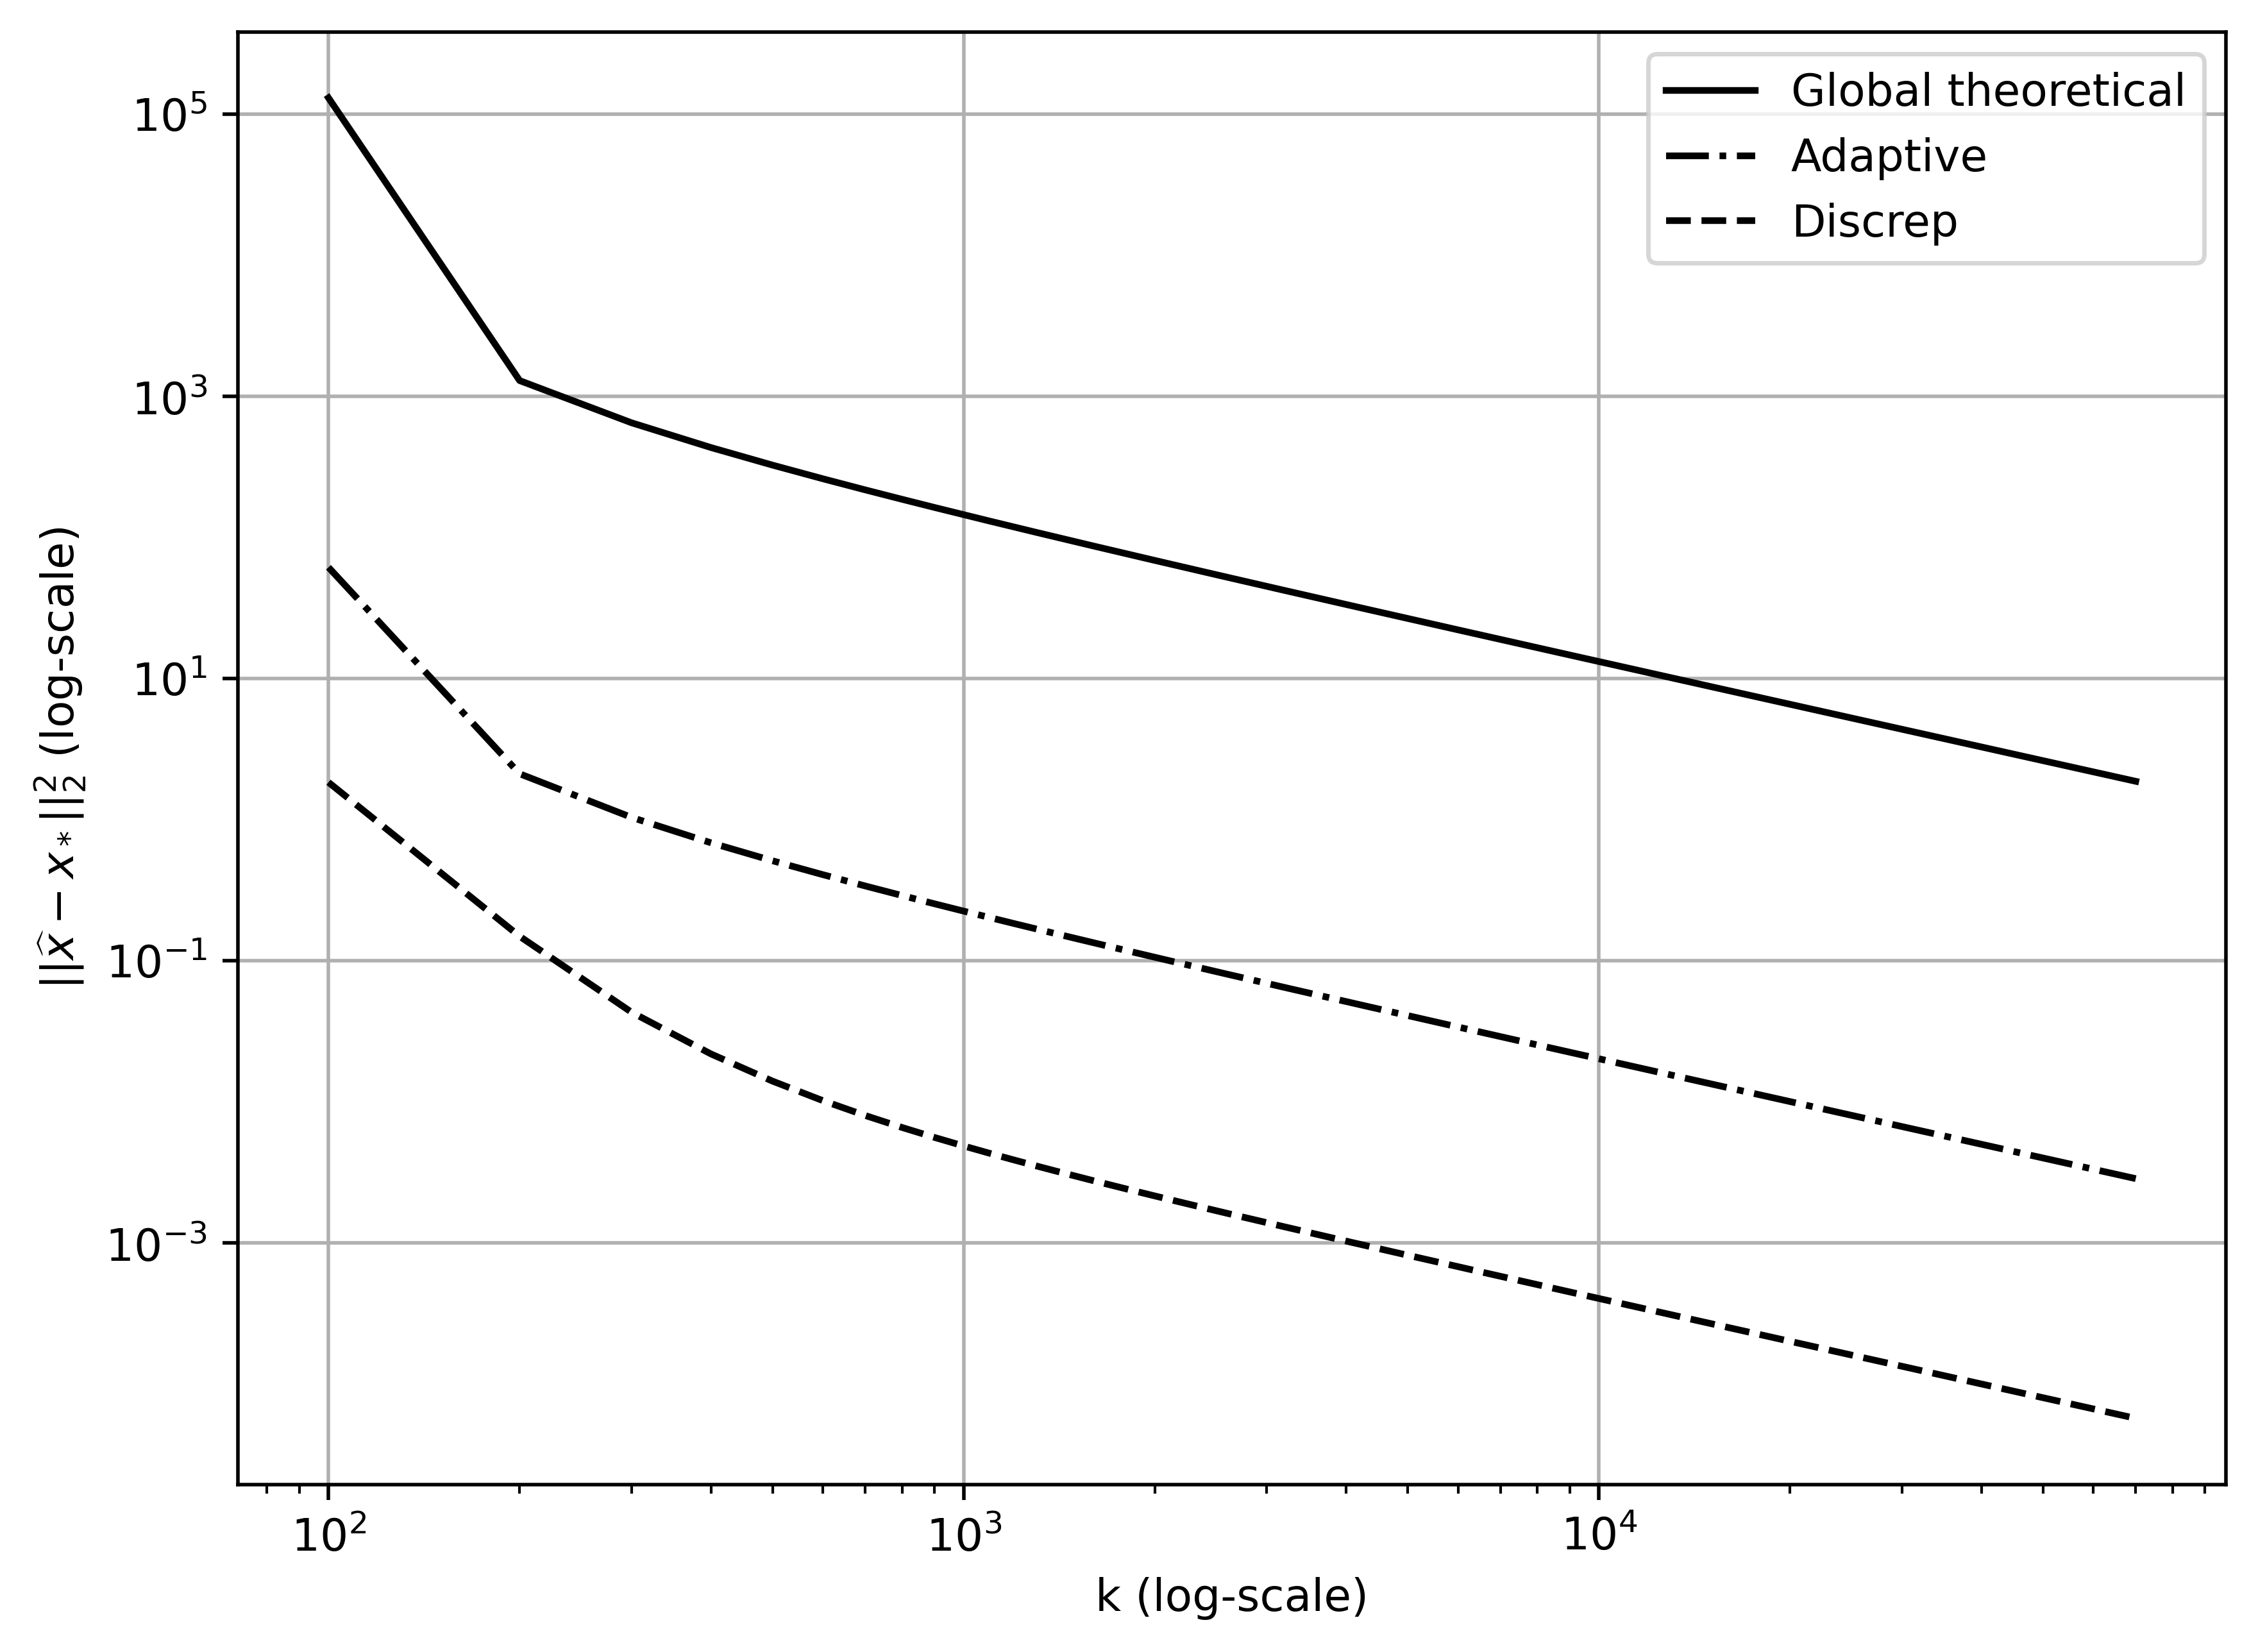
\includegraphics[width=\linewidth]{x_discr_rad_5_q_4_it_70_000_dim_1000.png}
        \endminipage\hfill
        \minipage{0.49\textwidth}
        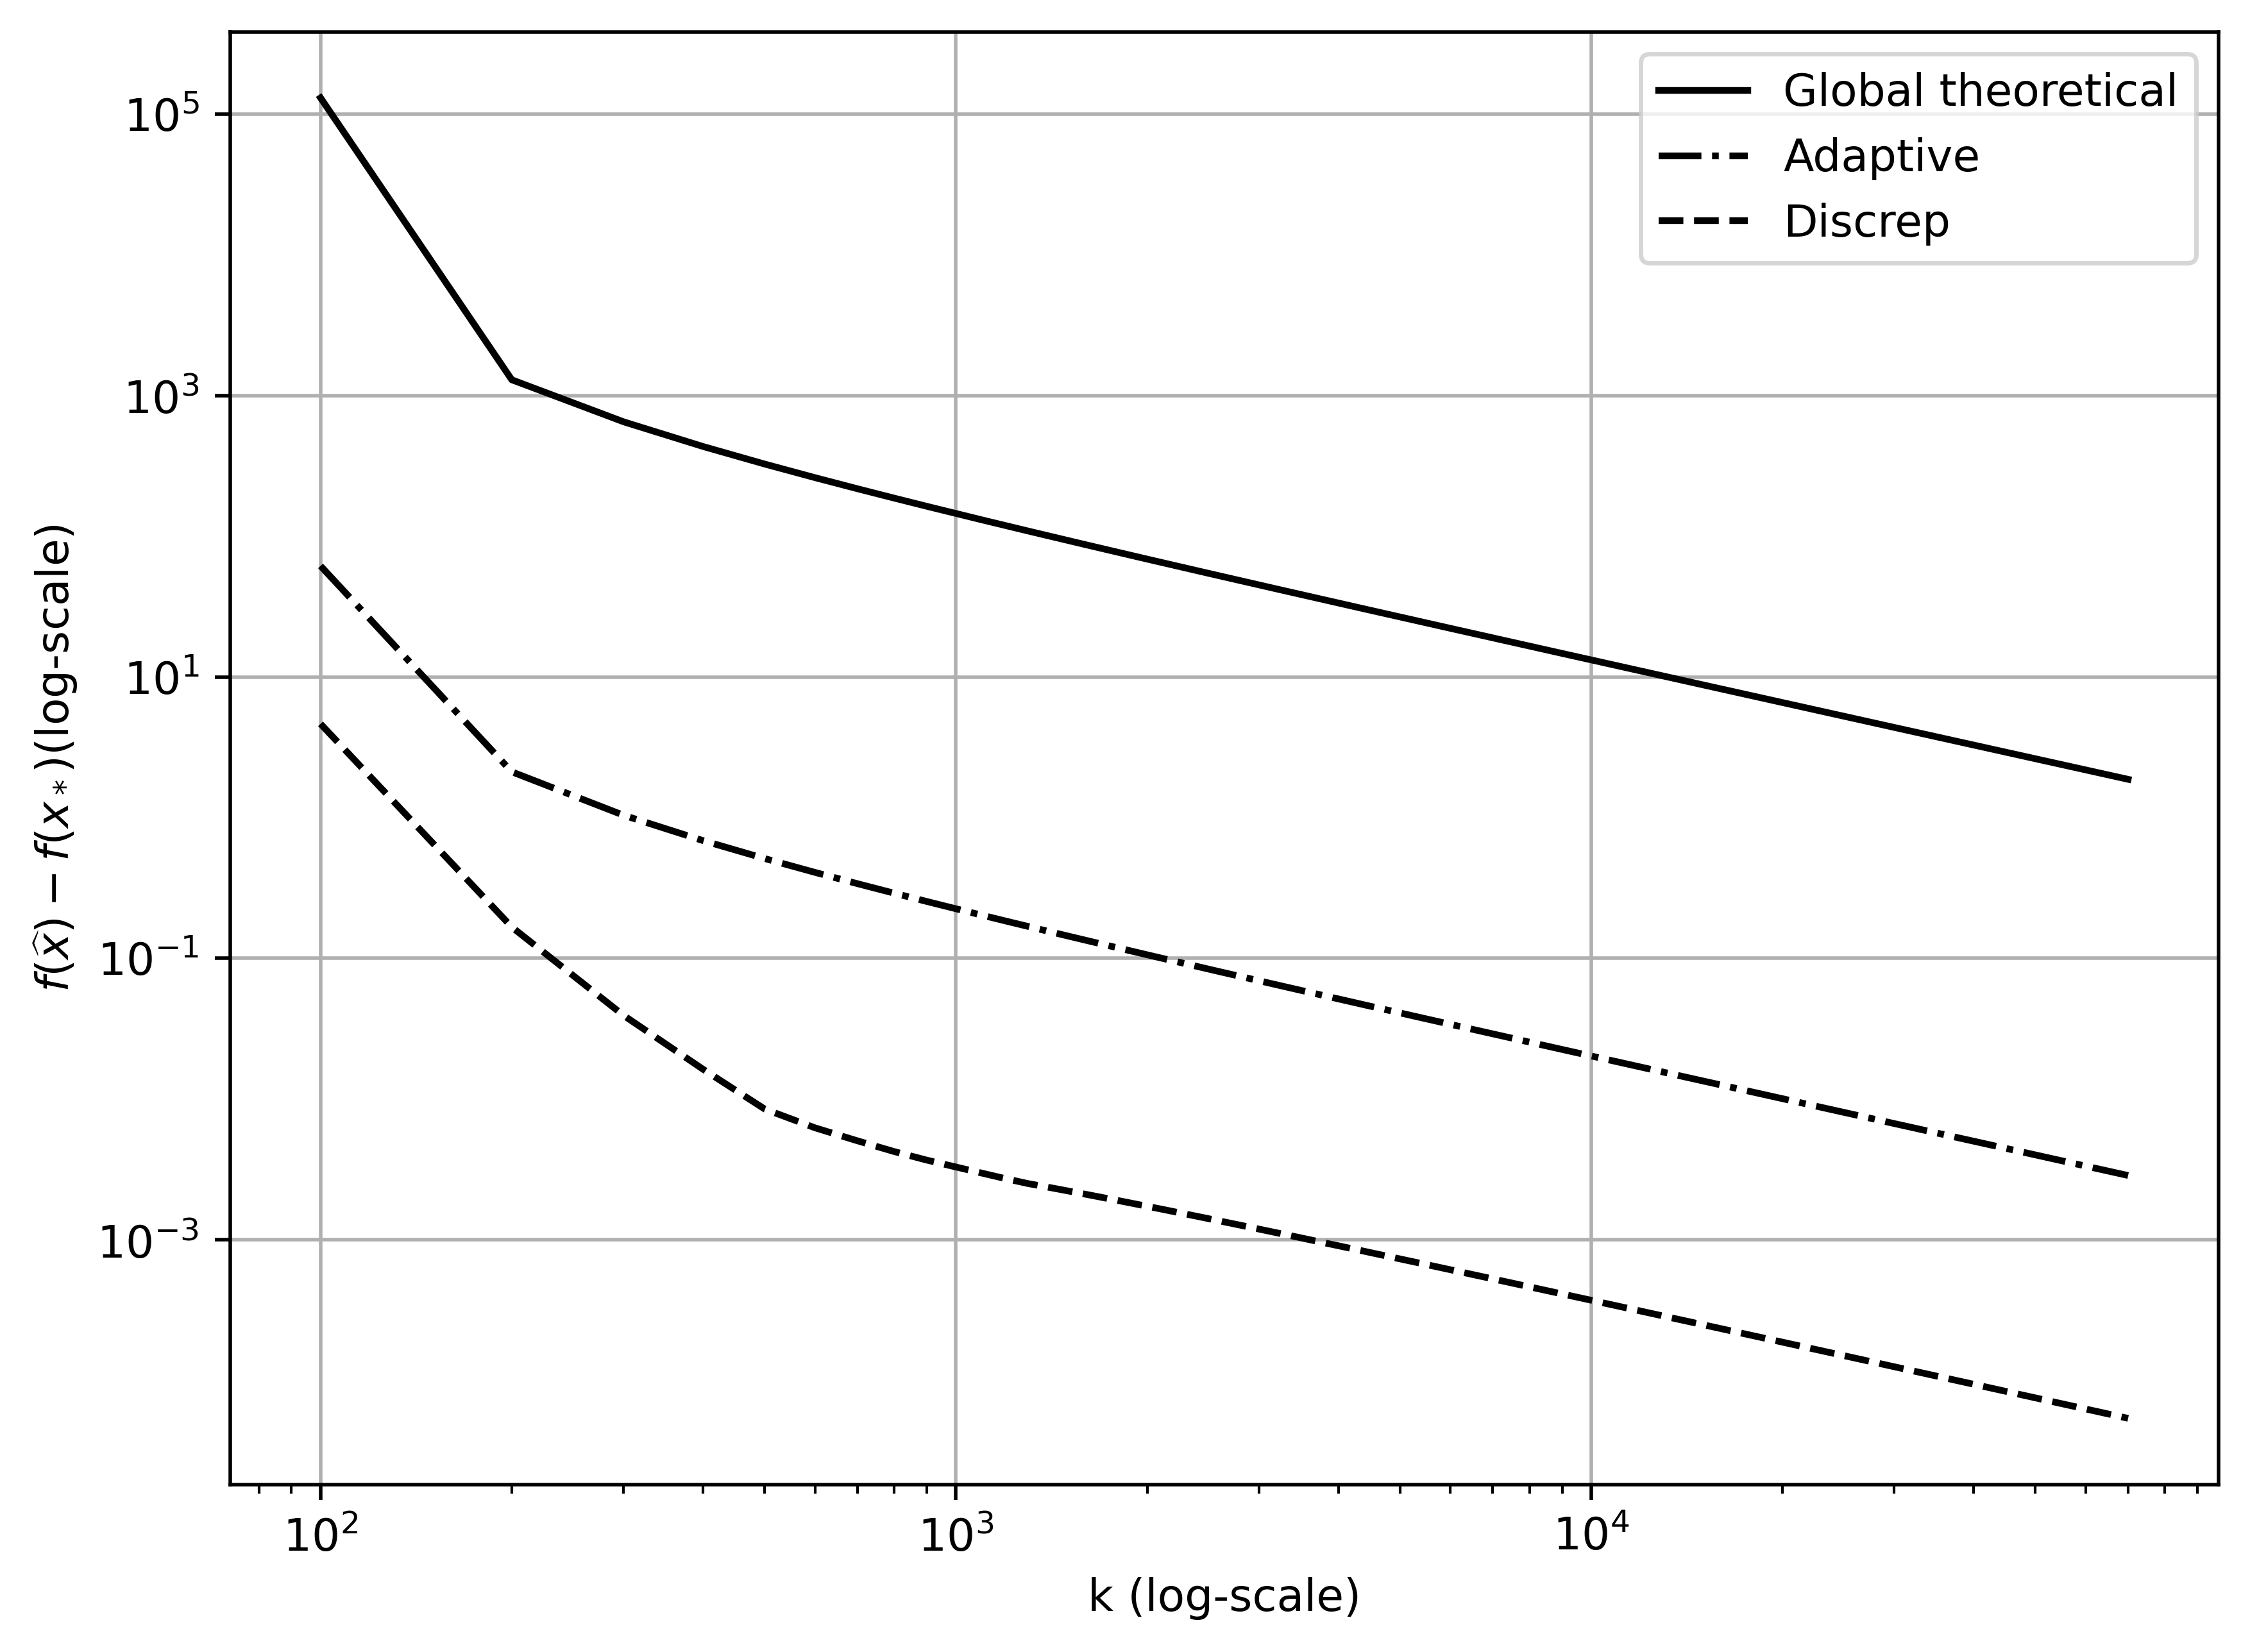
\includegraphics[width=\linewidth]{f_discr_rad_5_q_4_it_70_000_dim_1000.png}
        \endminipage\hfill
        \caption{Результаты решения задачи минимизации \eqref{sphere_cover_strongly}, где  $n= 1\,000, r = 5$ и  шар $Q$ радиуса 4.}
        \label{res_ex_strong_r5}
    \end{figure}

    \begin{figure}[h]
        \minipage{0.49\textwidth}
        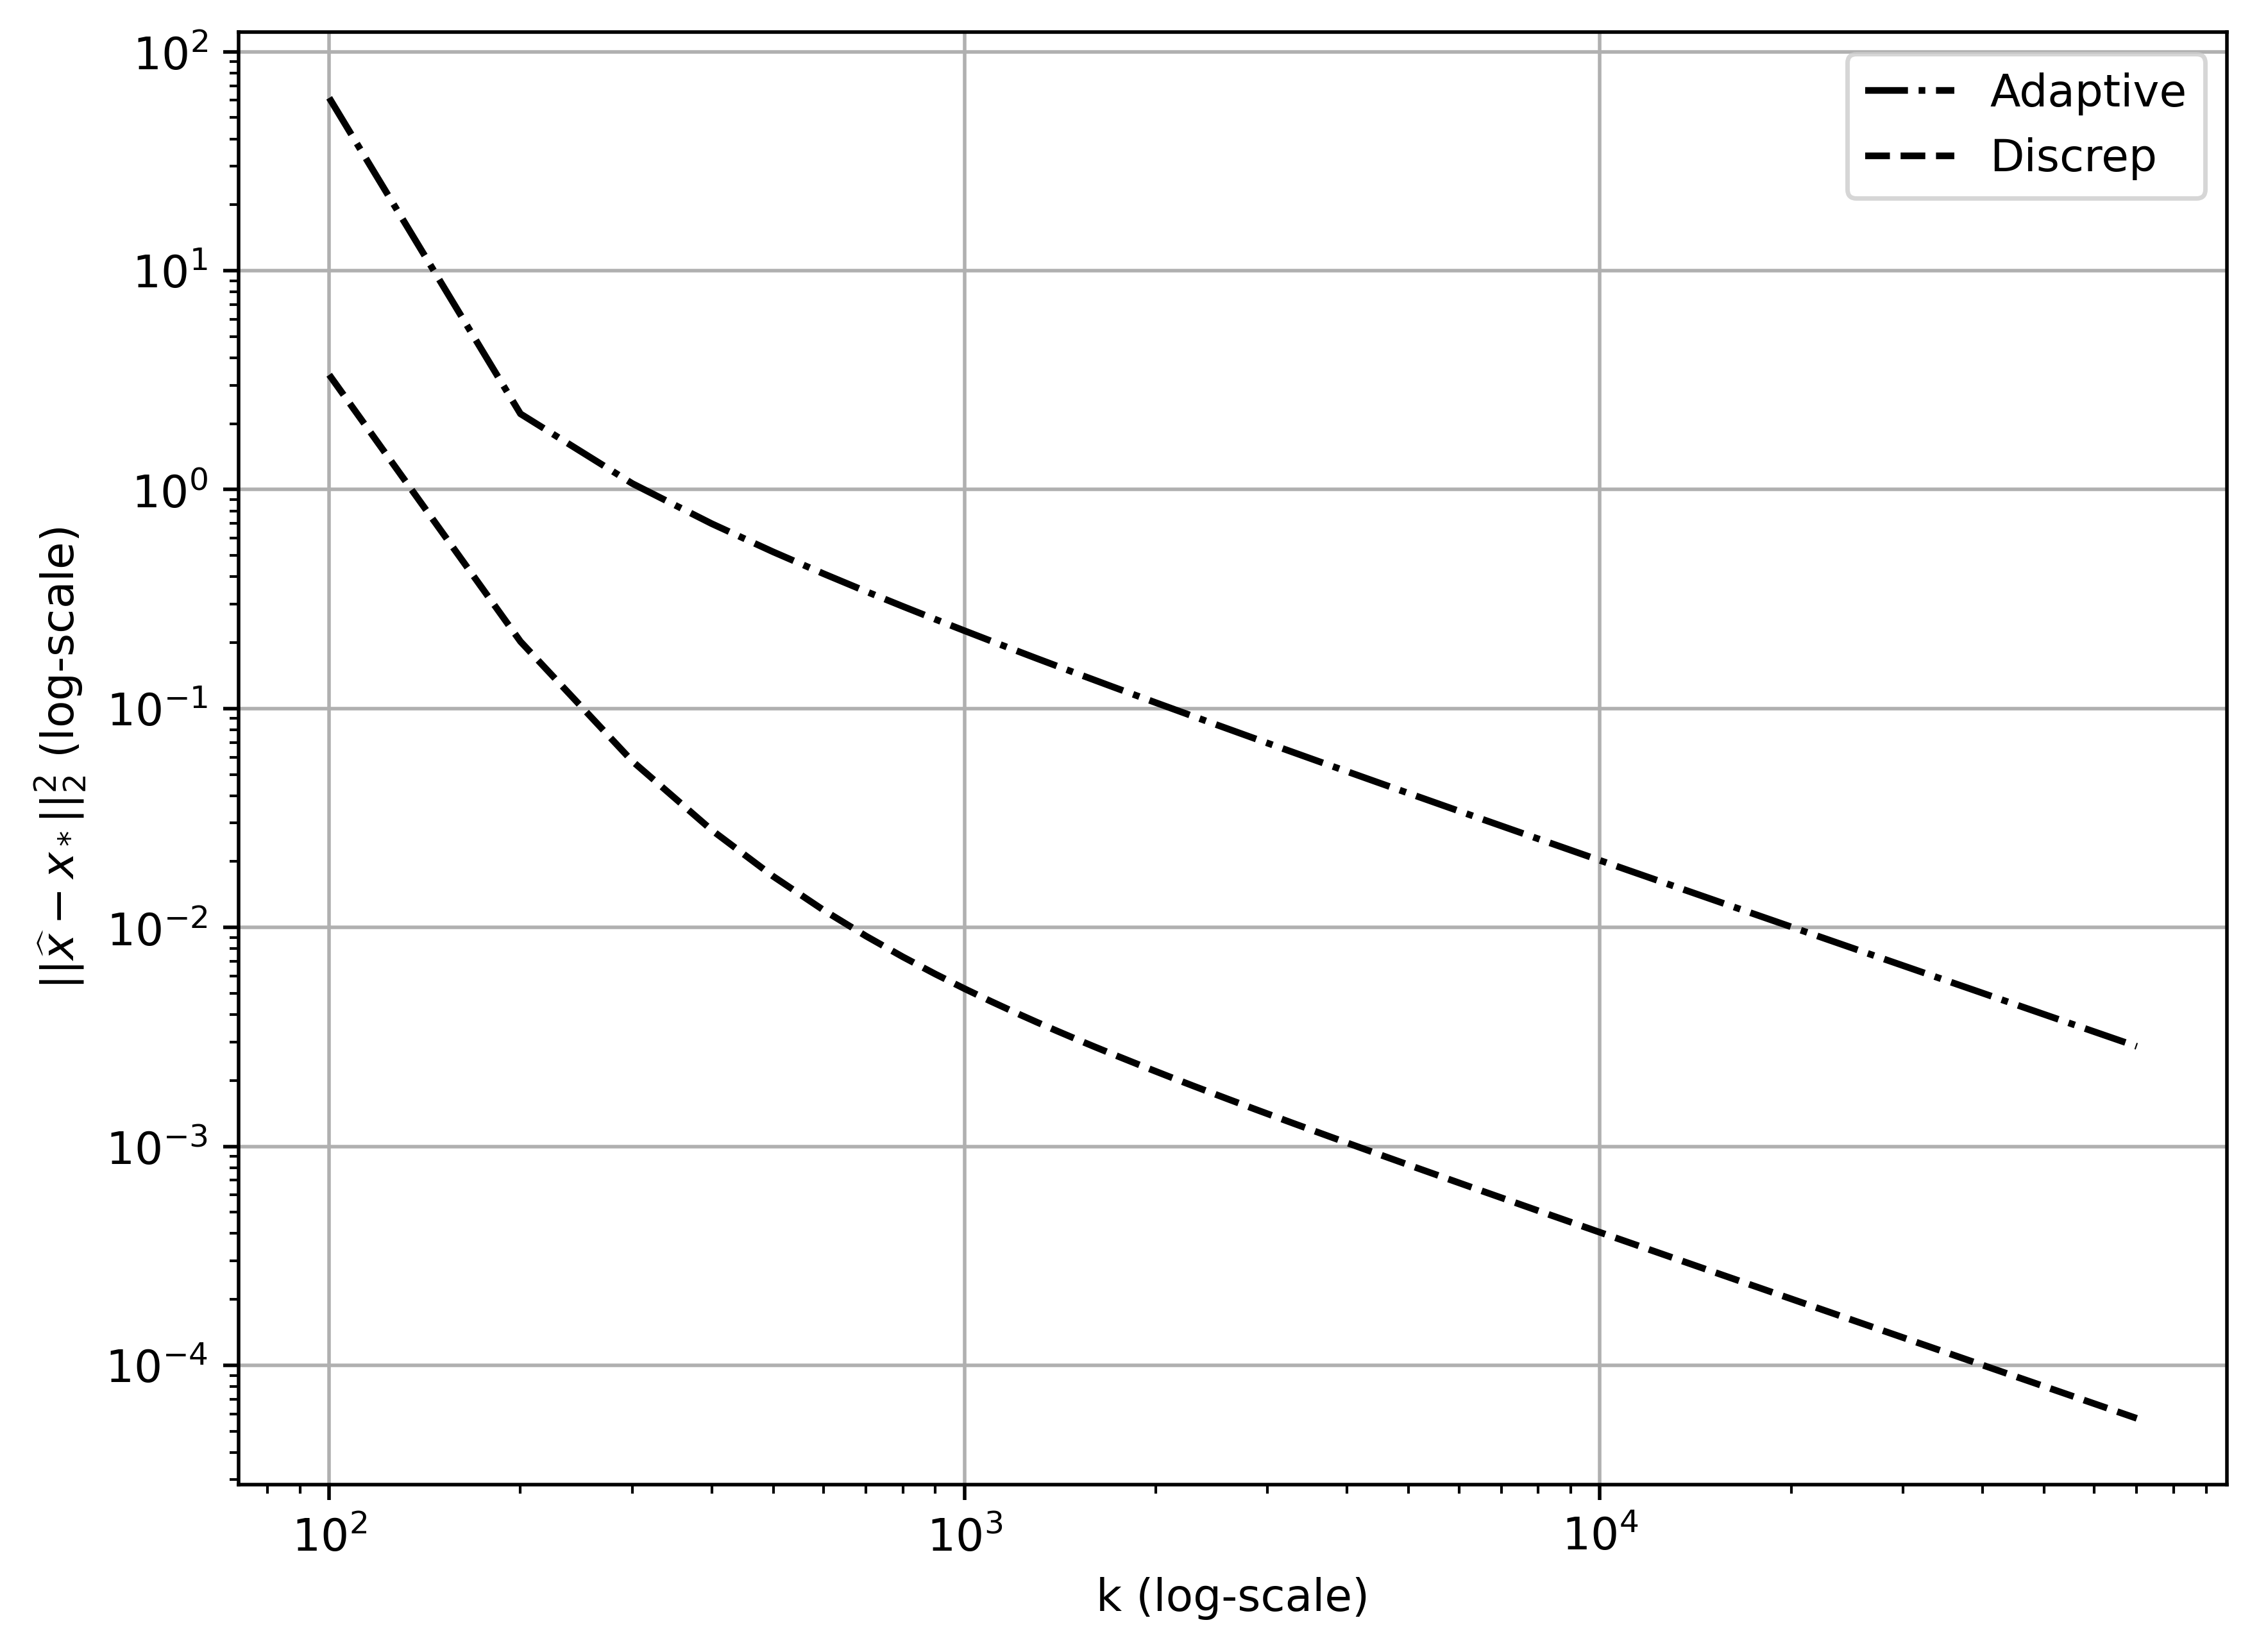
\includegraphics[width=\linewidth]{x_discr_unlim_q.png}
        \endminipage\hfill
        \minipage{0.49\textwidth}
        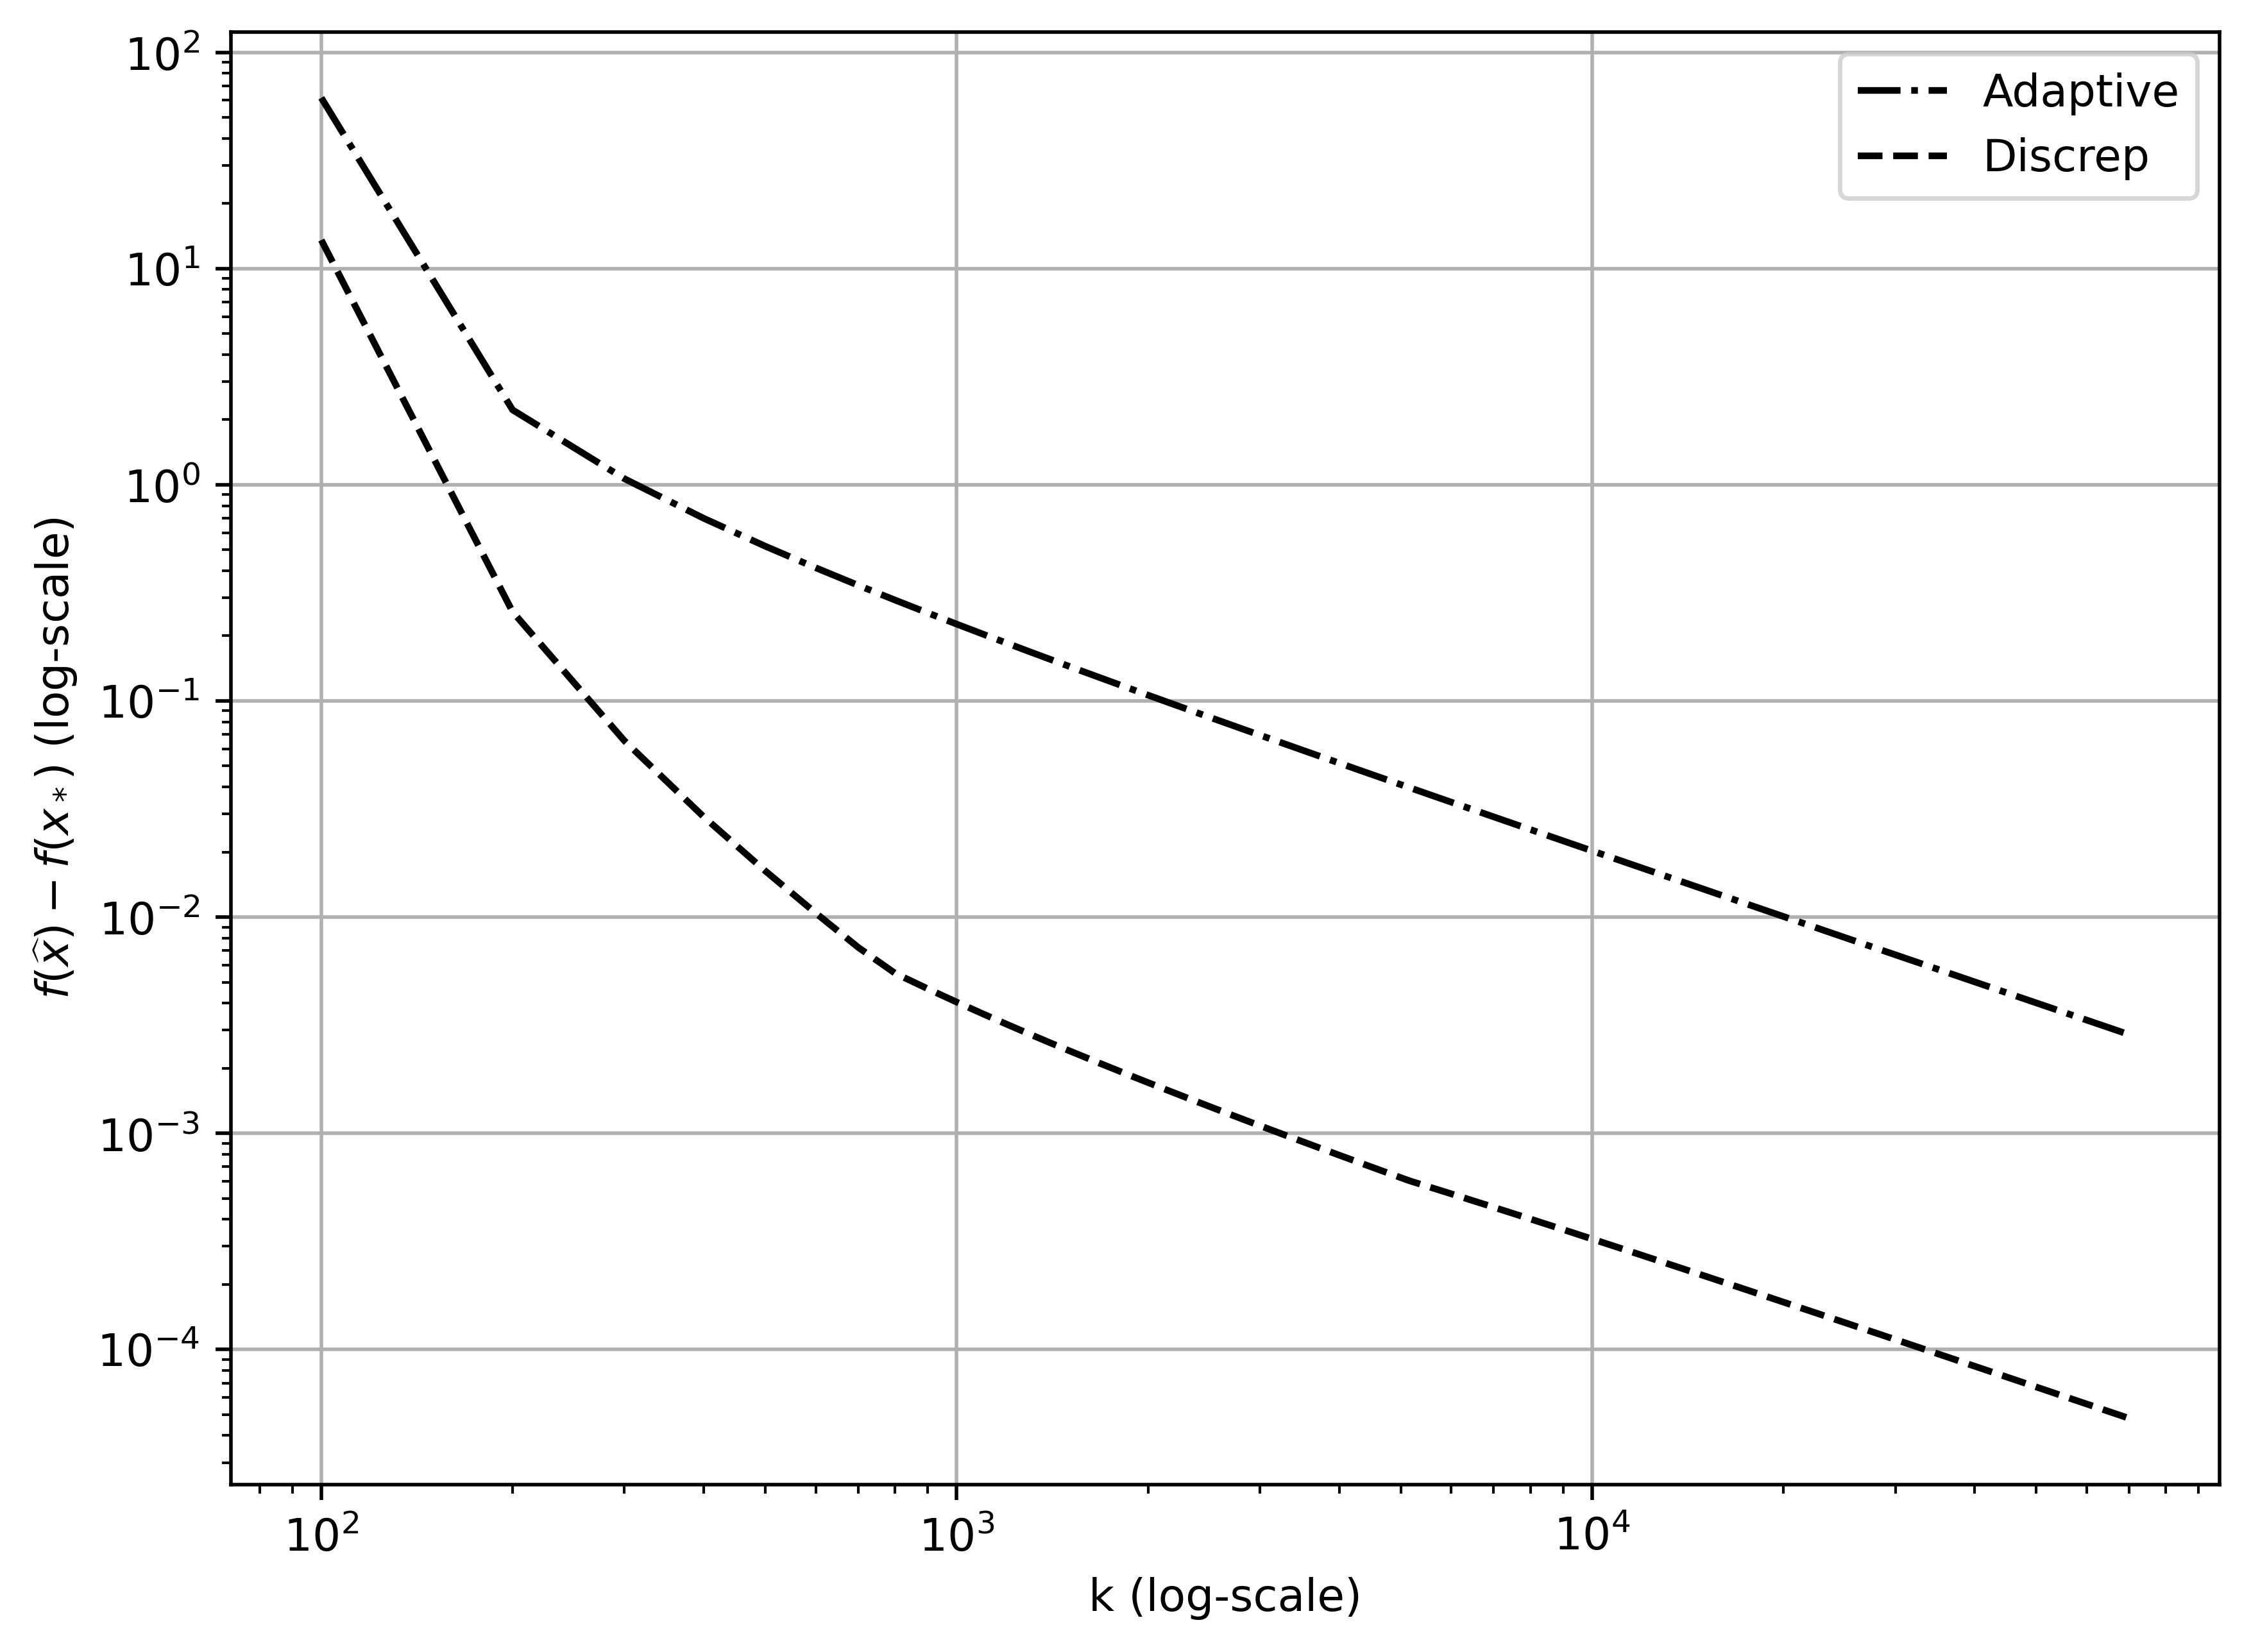
\includegraphics[width=\linewidth]{f_discr_unlim_q.png}
        \endminipage\hfill
        \caption{ Результаты решения задачи минимизации \ref{sphere_cover_strongly}, где  $n= 1\,000, r = 5$ и  $Q = \mathbb{R}^n$.}
        \label{res_ex_strong_unlim}
    \end{figure}

    Теперь перейдём к выпуклой постановке \eqref{sphere_cover} с целью исследования эффективности предложенных в разделе 3 субградиентных методов с $\Delta$-острым мнимимумом. К существующему набору точек, представленных для покрытия, с известным значением центра добавим дополнительную точку, которая находится вне исходного шара достаточно близко к границе (удалена не более, чем на $\Delta > 0$). Данный подход позволяет оценить <<приближённое>> значение минимума $\overline{f}$, что позволит применить разработанные выше варианты субградиентного метода с $\Delta$-острым минимумом. При этом новое значение минимума останется внутри исходной сферы. Поскольку оптимальное значение функции --- это радиус искомого шара, покрывающего все точки, а $x_*$ всегда будет расположена внутри него, то для всякого $x$ верно неравенство $ f(x) \geq \| x - x_*\|_2$. Рассмотрим целевую функцию вида
    \begin{gather}\label{allpha_sphere_cover}
        f(x) := \alpha \max_{x\in Q}\{\|x - a_0\|_2, \|x - a_1\|_2, ..., \|x - a_m\|_2\}.
    \end{gather}
    Тогда значение $\Delta$ можно оценить  из (\ref{eq_gen_sharp}): 
        $f(x) - \overline{f} \geq \alpha\|x- x_*\|_2 - \Delta, \quad \Delta \geq \overline{f}$.

    Отметим, что данная постановка значительно влияет на величину теоретической оценки качества решения (\ref{adaptive_estimate}) для метода \eqref{1}.
    Наиболее значимый вклад в оценку (\ref{adaptive_estimate}) дает последнее слагаемое $\frac{\Delta^2}{2\|\nabla f(x_k)\|^2_2}$, причём 
    $     \Delta \sim \overline{f} \sim \alpha \|\overline{x}-a\|_2 $ и 
    $     \|\nabla f(x_k)\|_2 = \alpha $. Поэтому последнее слагаемое пропорционально радиусу шара, соответсвующему <<приближённому>> решению. Это и подтверждается экспериментально. Для сравнения, ниже на рис. \ref{res_sharp_convex} и \ref{res_strong_convex} приведены результаты работы для того же набора входных точек, которые необходимо покрыть в обоих постановках --- (\ref{allpha_sphere_cover}) и (\ref{sphere_cover_strongly}). Начальная точка также одна и та же. Сравниваются методы \eqref{1} и \eqref{orig}. Первый из этих методов обеспечивает сходимость буквально за 10 итераций к <<приближённому>> решению с заданной точностью и даже позволяет эту точность повысить. Второй же метод достигает схожих (с геометрической точки зрения) результатов за значительно большее количество итераций, однако он позволяет повышать точность приближённого решения на дальнейших итерациях.

    Подтверждение данного теоретического наблюдения хорошо иллюстрируется на рис. \ref{res_sharp_convex} и \ref{res_strong_convex}. На рис. \ref{res_sharp_convex} показано поведение субградиентного спуска, использующего $\Delta$-острый минимум (теорема \ref{theorem4}), а именно --- быстрая сходимость к <<приближенному>> решению. Штрих-пунктирная линия соответствует оценке \eqref{eq_gen_sharp}, а штриховая --- невязке по функции и аргументу. На рис. \ref{res_strong_convex} показано поведение метода для той же задачи, но с использованием сильно выпуклого целевого функционала (теорема \ref{ThmBachAdaptive}). Скорость убывания уже не столь высокая, но точность получаемого решения в итоге выше. Сплошная линия --- это глобальная оценка \eqref{orig_estimation_f}, штрих-пунктирная --- адаптивная \eqref{adaptive_estimation_f}, а штриховая --- невязка по функции и аргументу.

    \begin{figure}[h]
        \minipage{0.49\textwidth}
        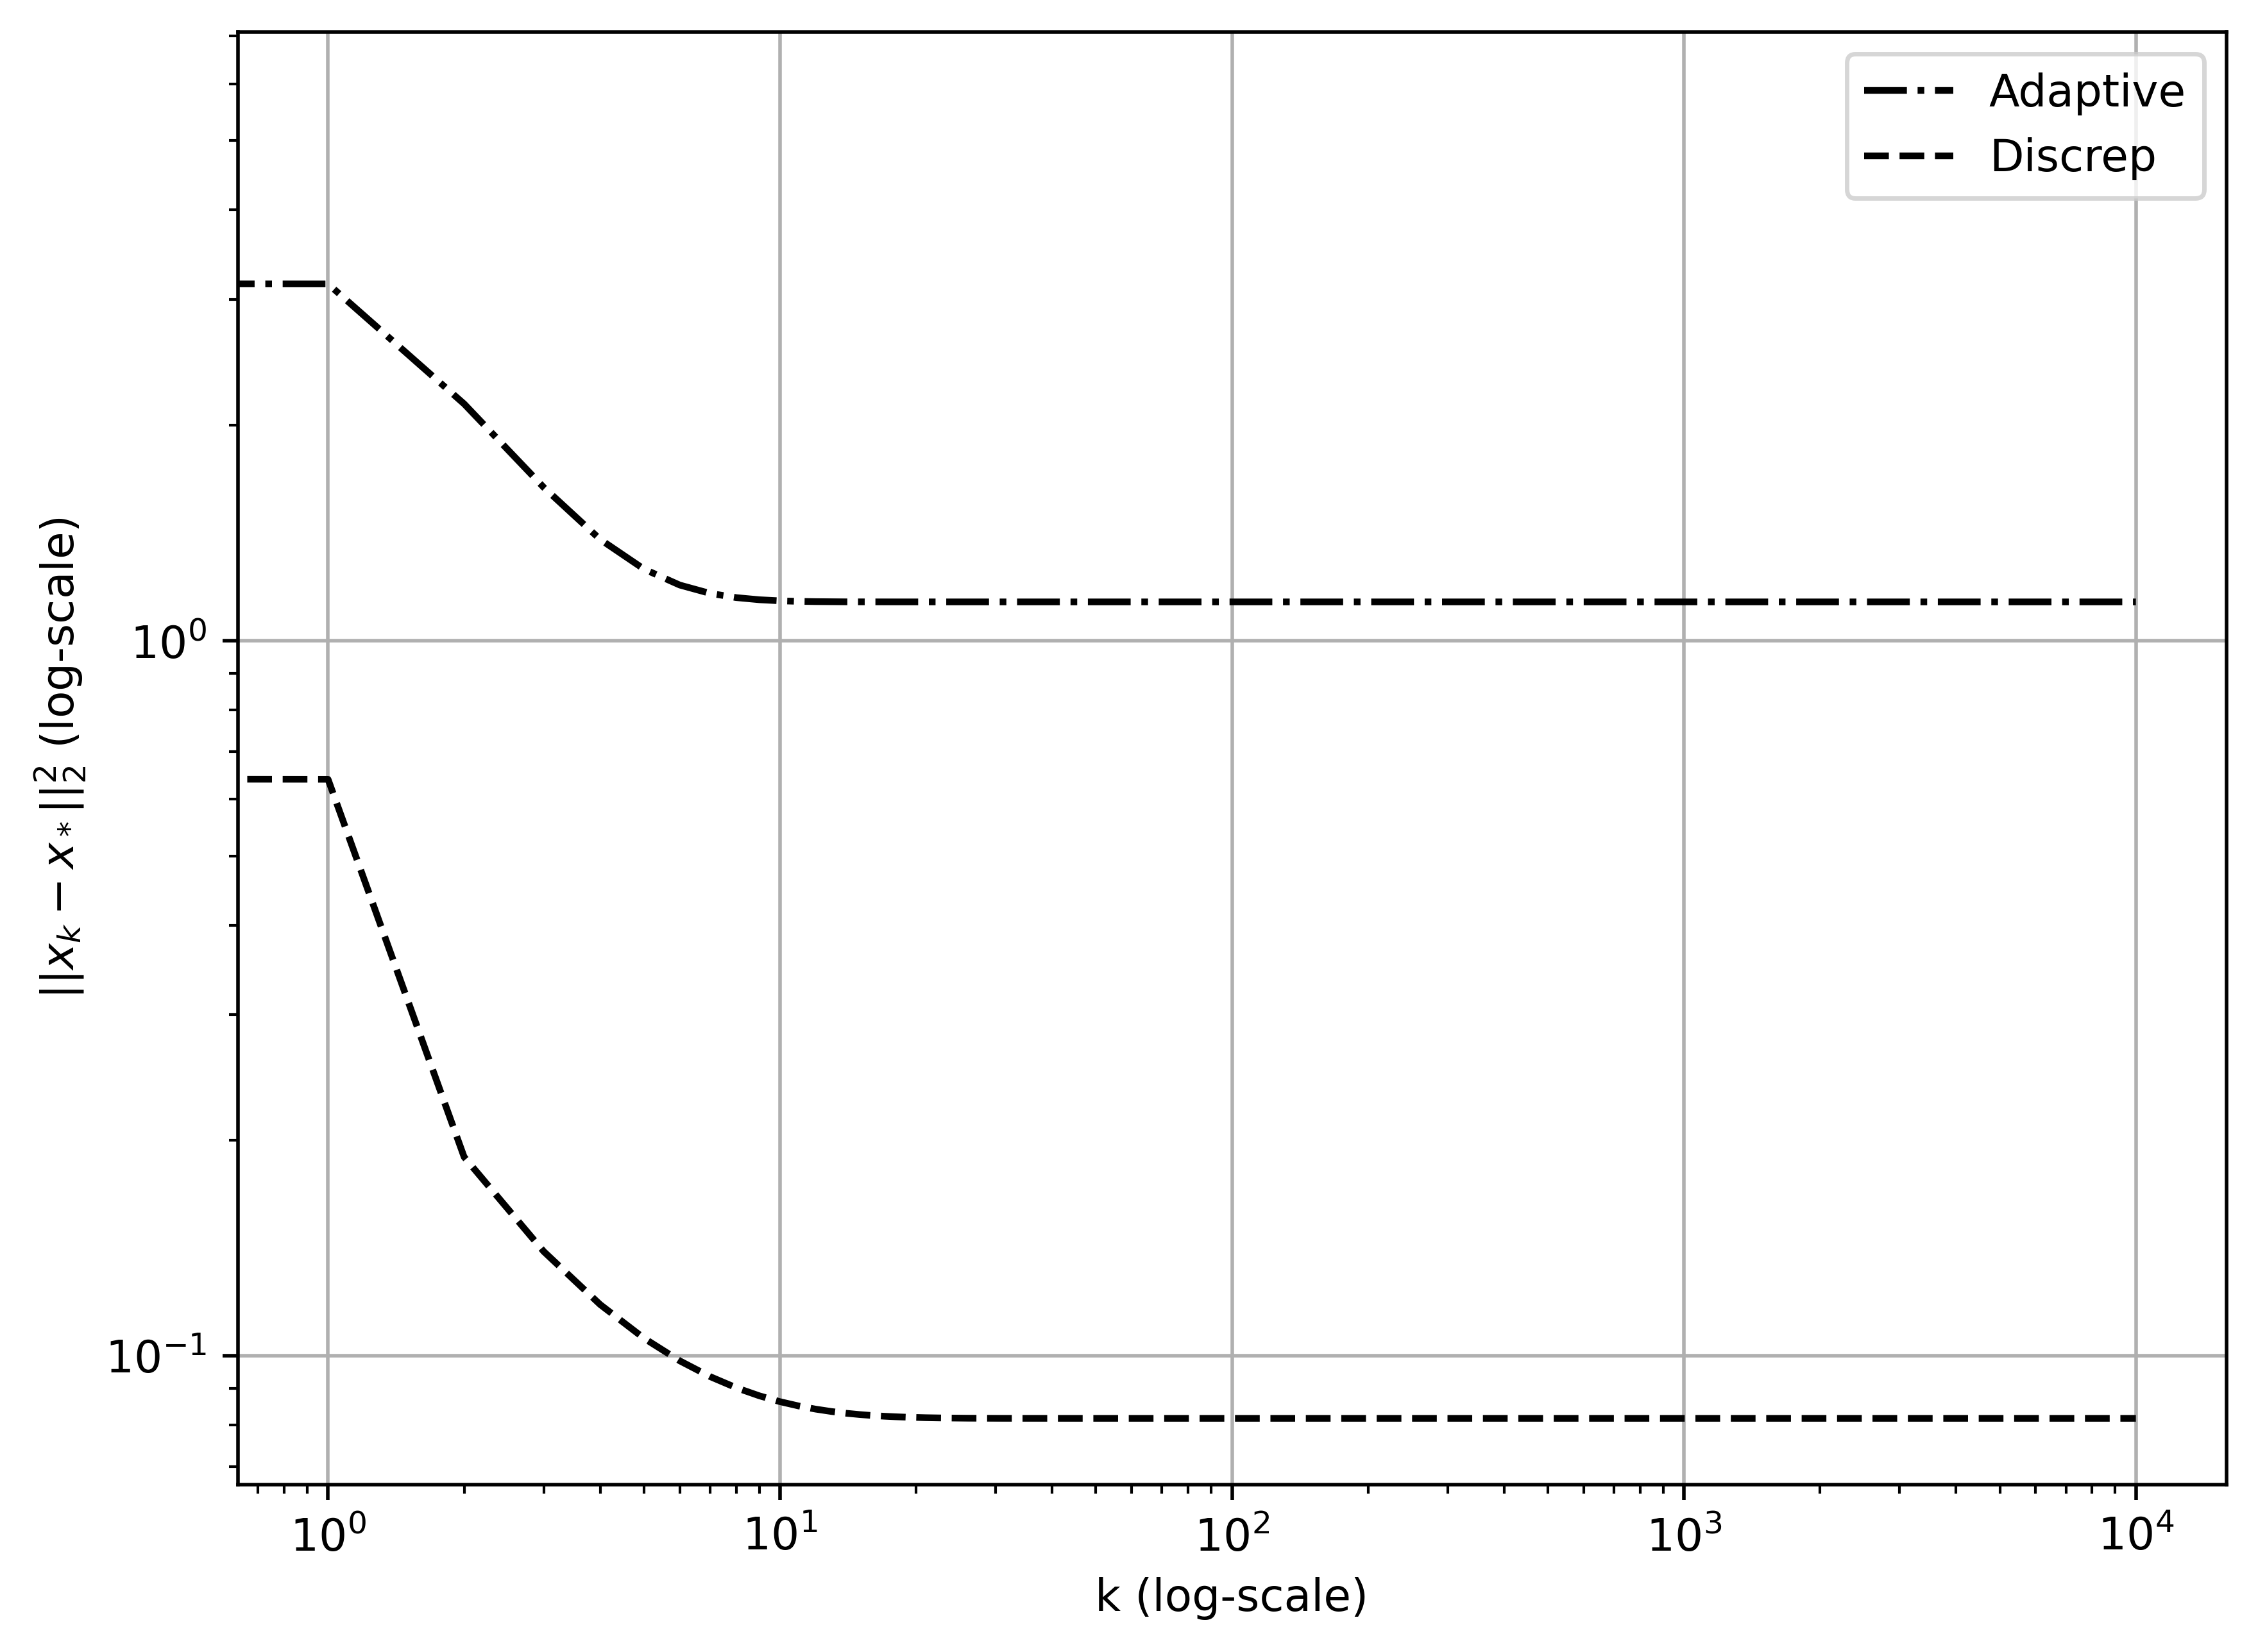
\includegraphics[width=\linewidth]{sharp_convex_x.png}
        \endminipage\hfill
        \minipage{0.49\textwidth}
        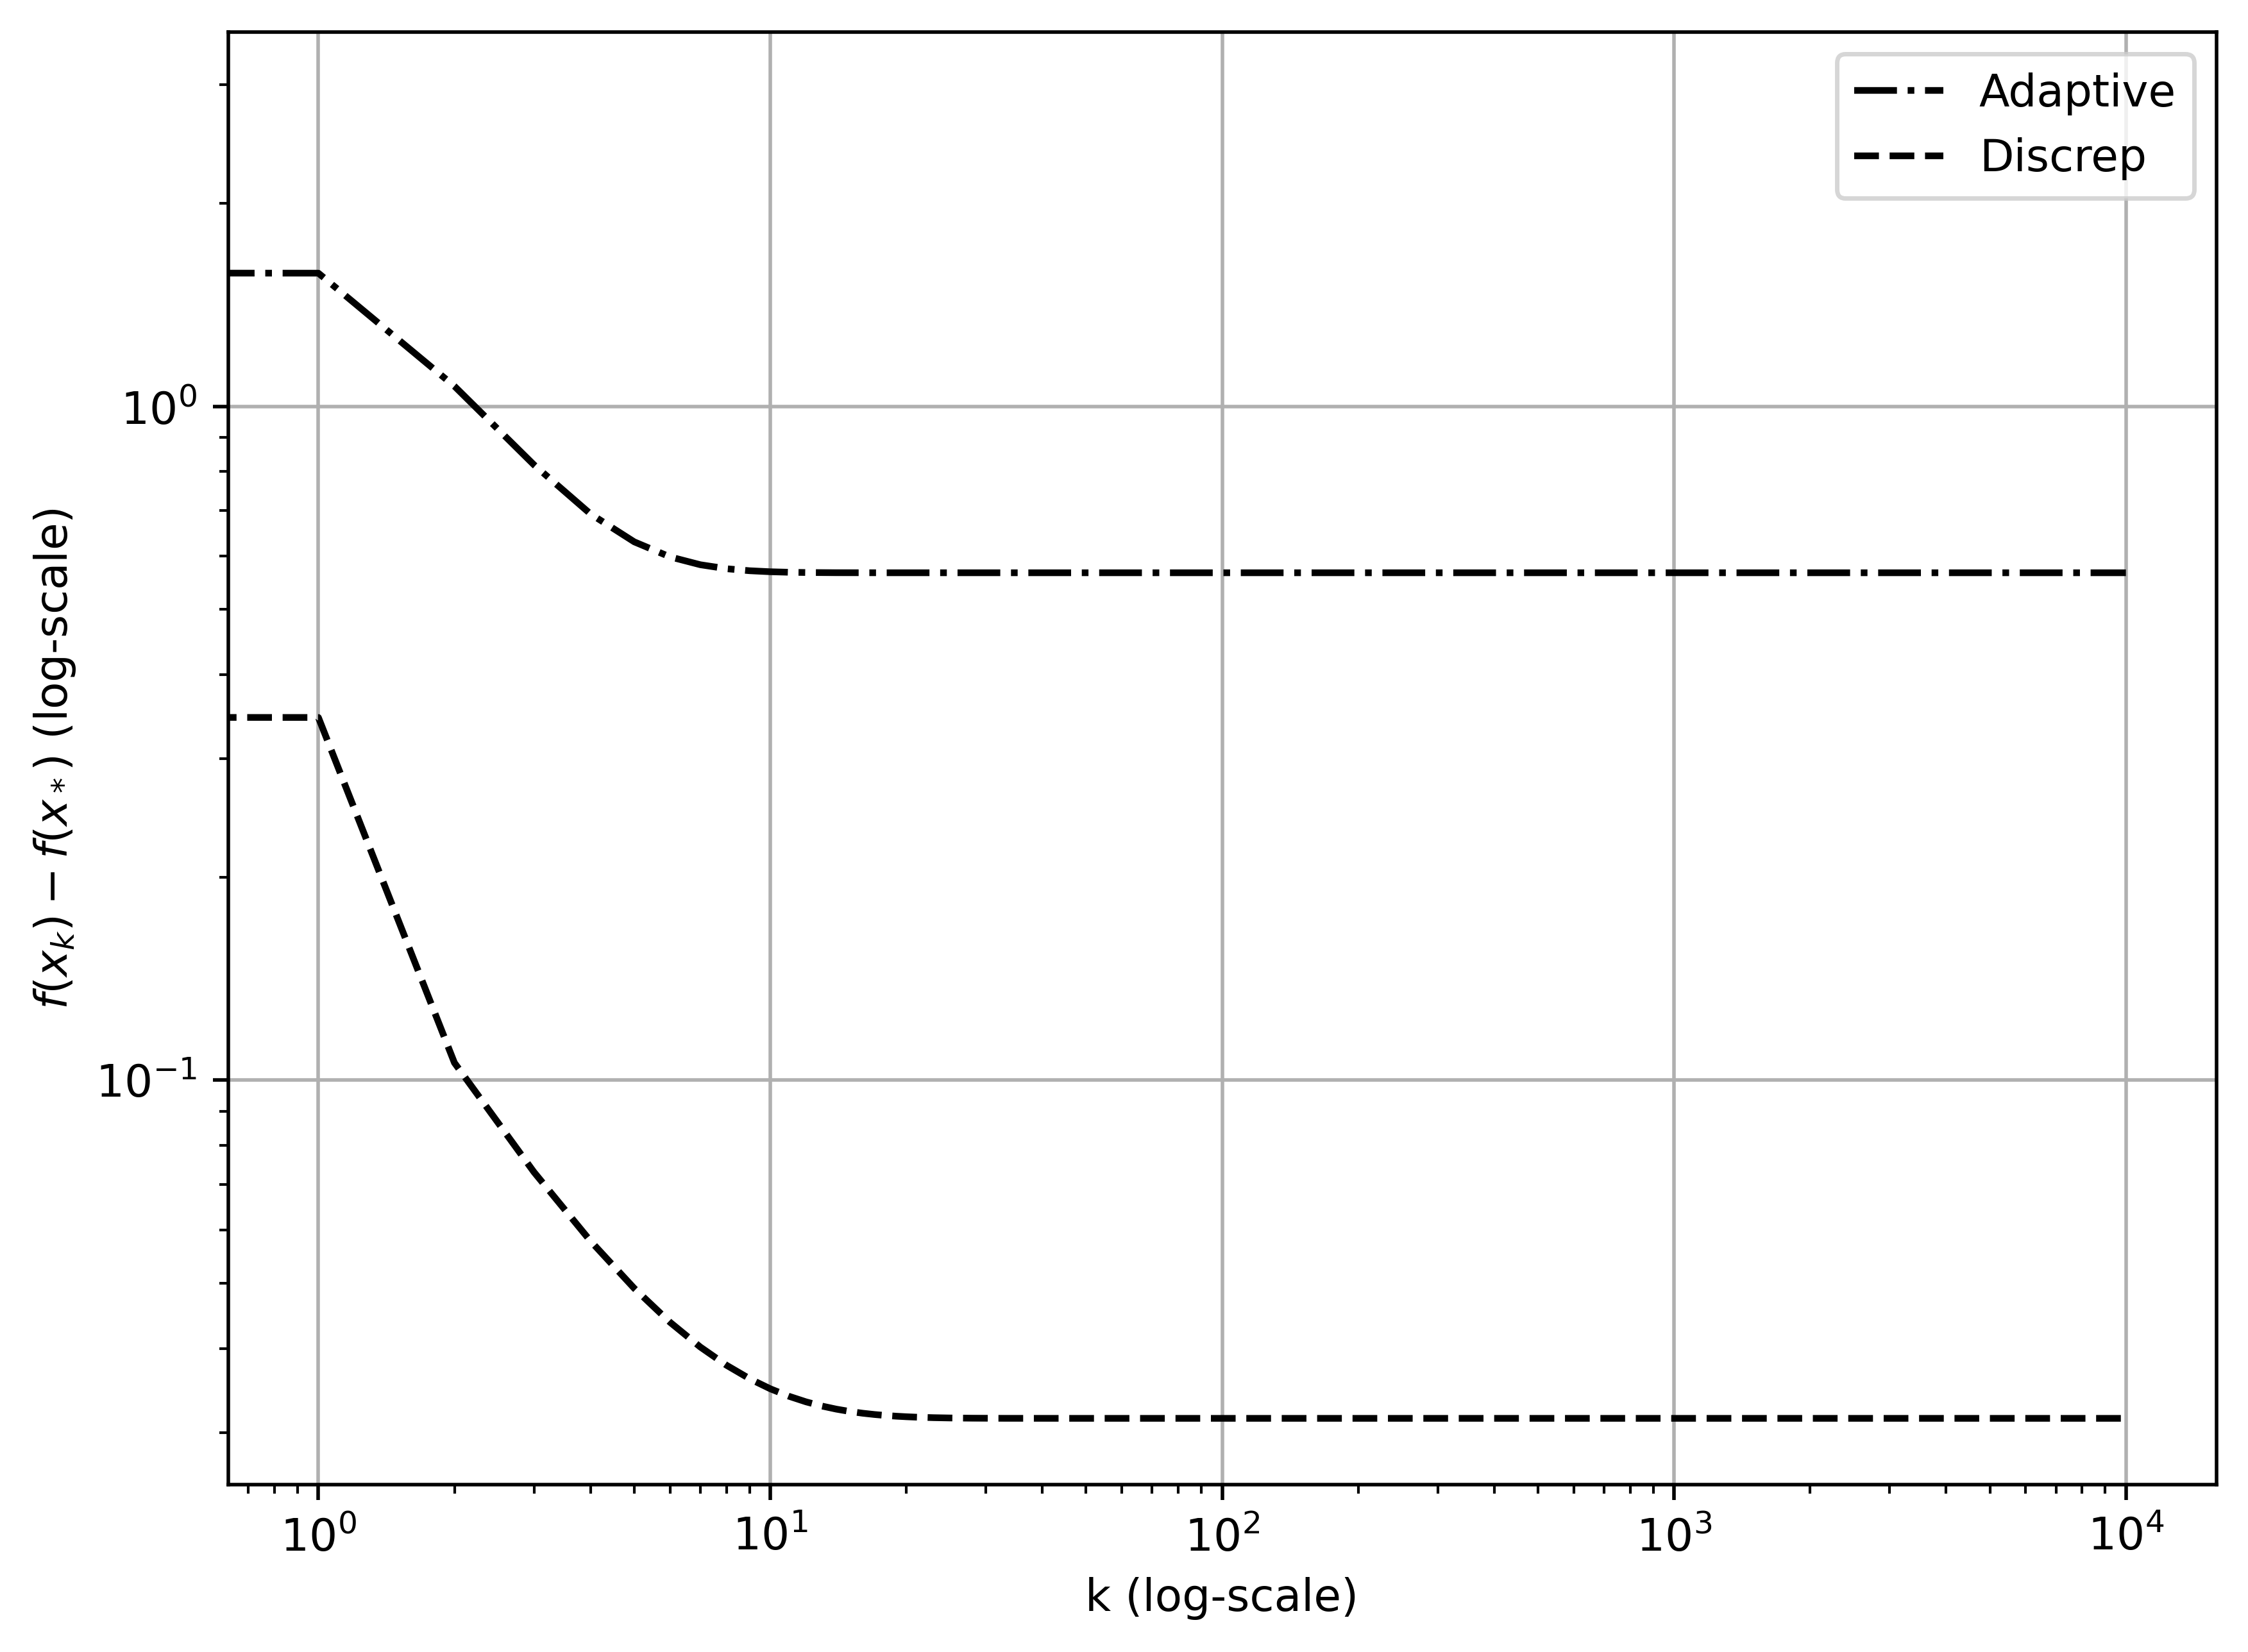
\includegraphics[width=\linewidth]{sharp_convex_f.png}
        \endminipage\hfill
        \caption{ Результаты решения задачи минимизации (\ref{allpha_sphere_cover}), где  $n= 1\,000, r = 0.7525, \alpha = 0.6$.}
        \label{res_sharp_convex}
    \end{figure}

    \begin{figure}[h]
        \minipage{0.49\textwidth}
        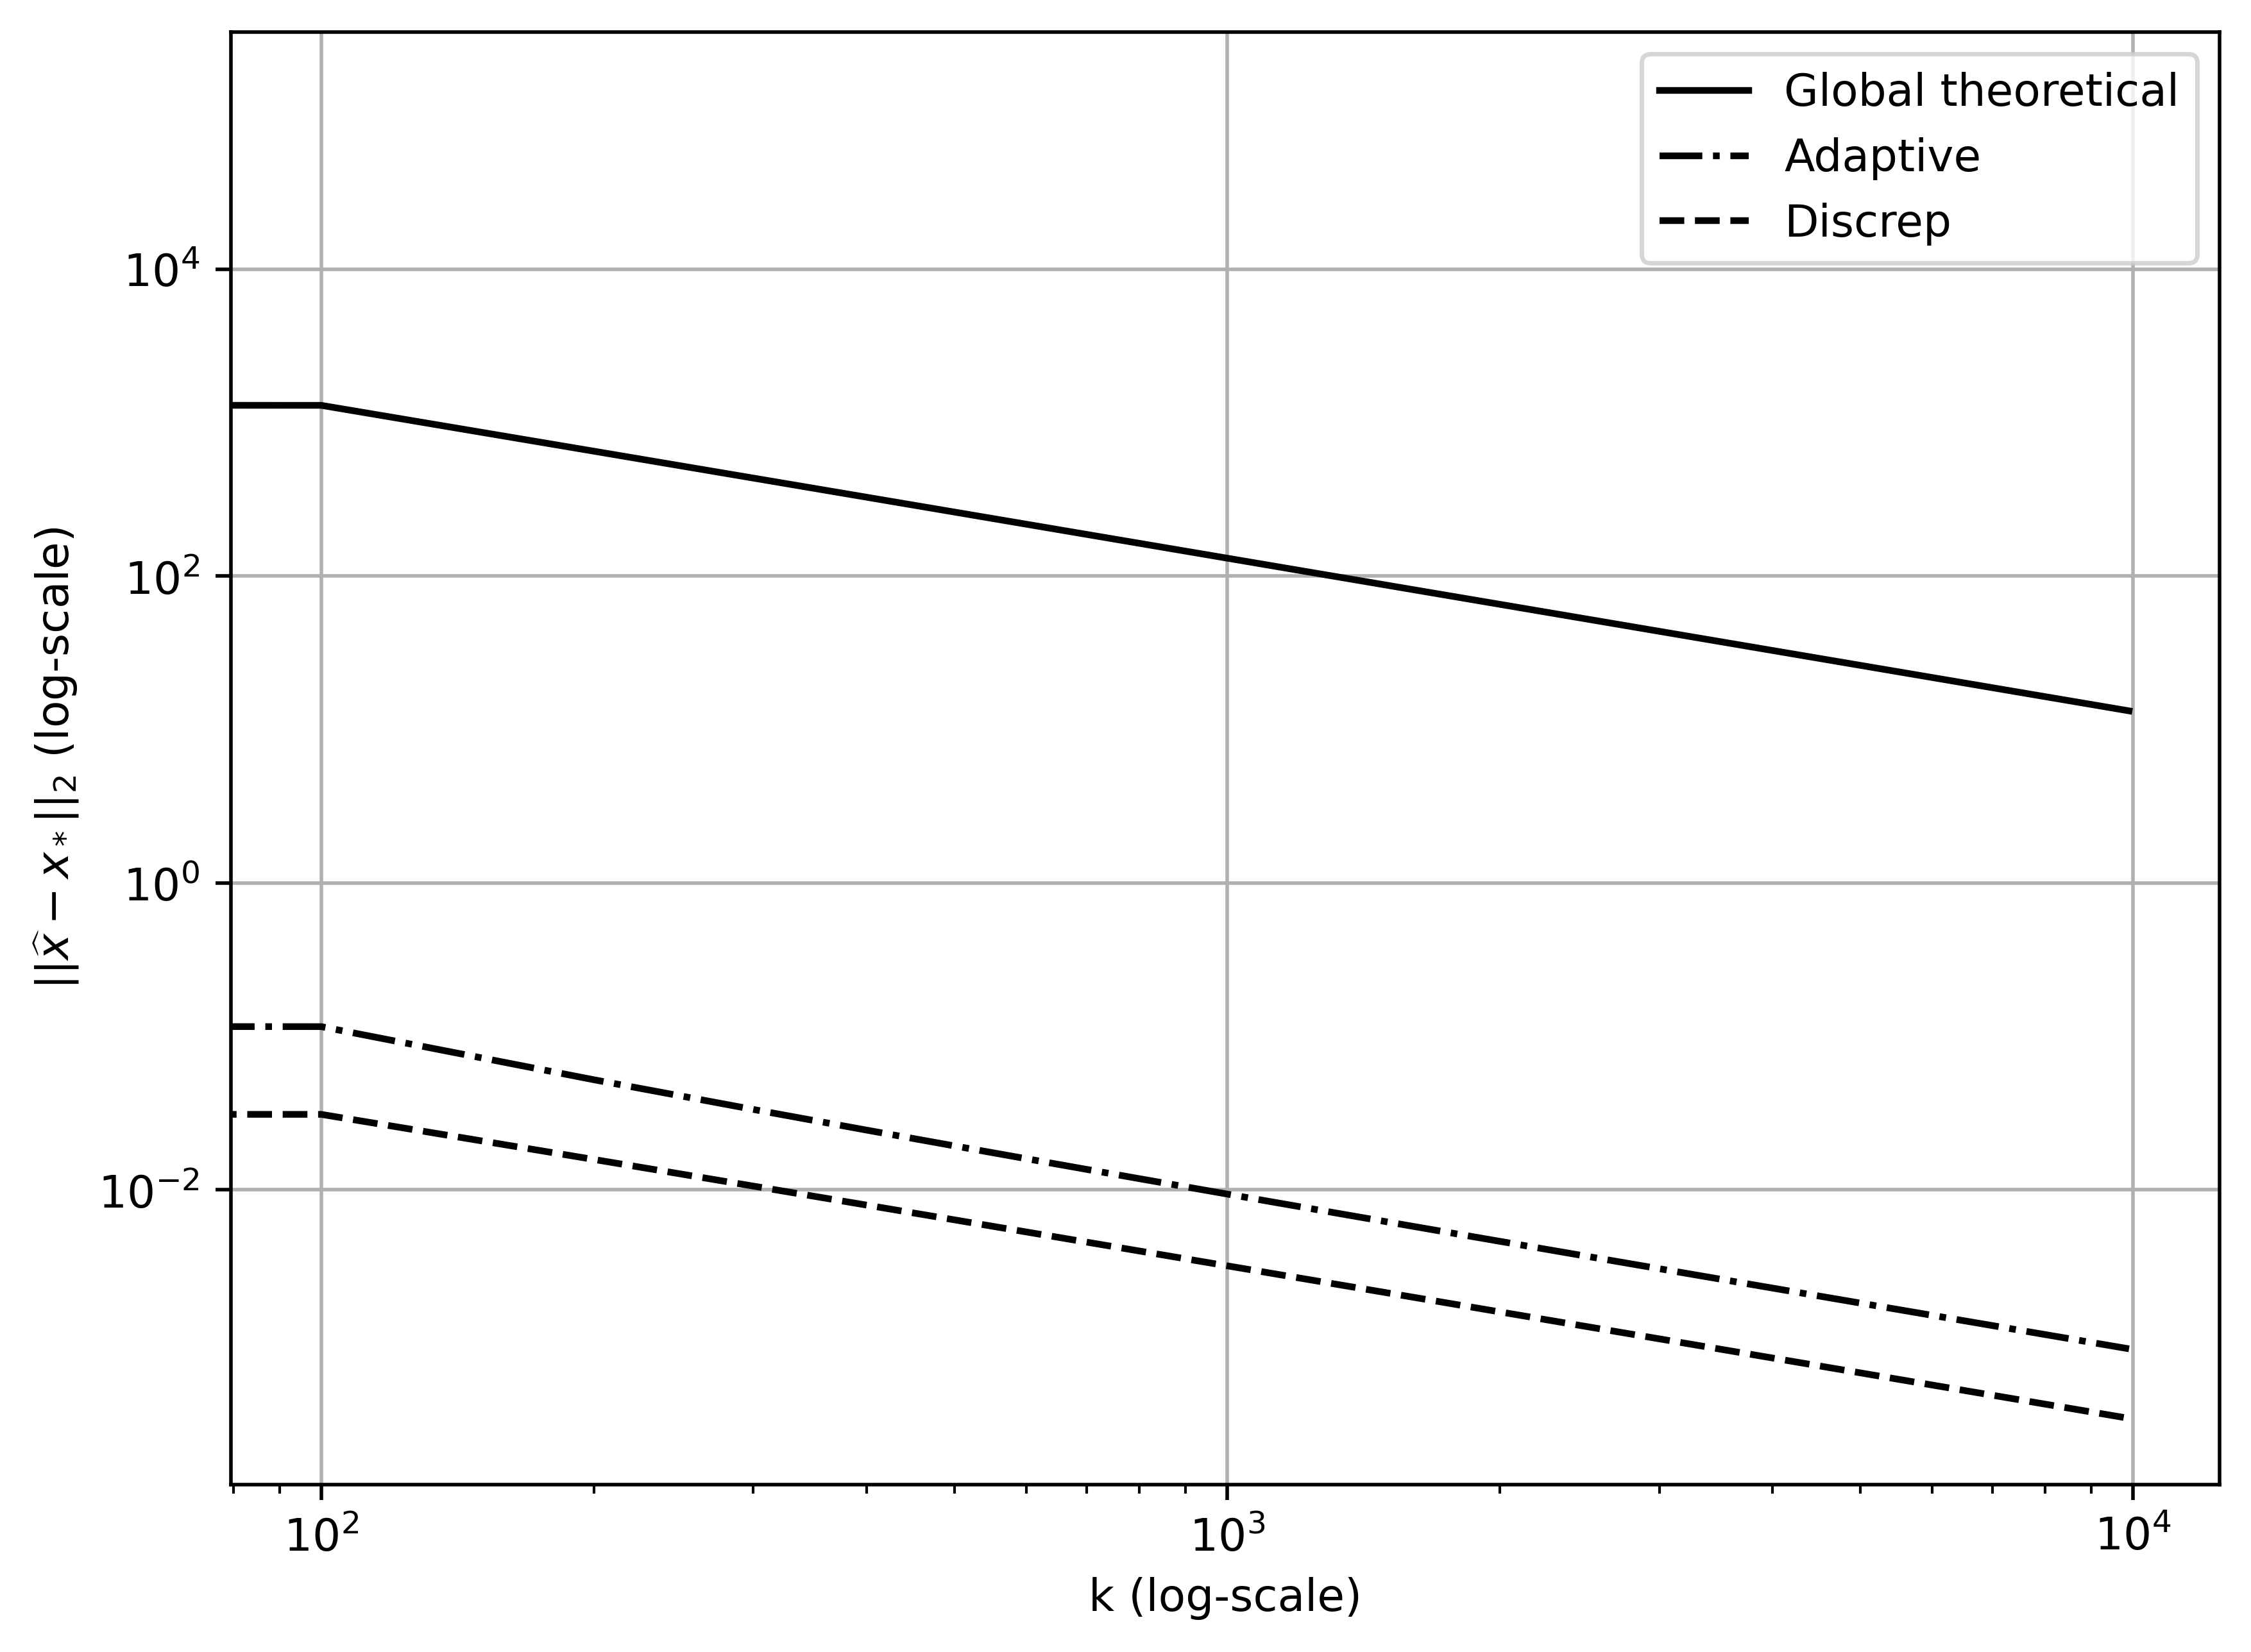
\includegraphics[width=\linewidth]{strong_convex_small_rad_x.png}
        \endminipage\hfill
        \minipage{0.49\textwidth}
        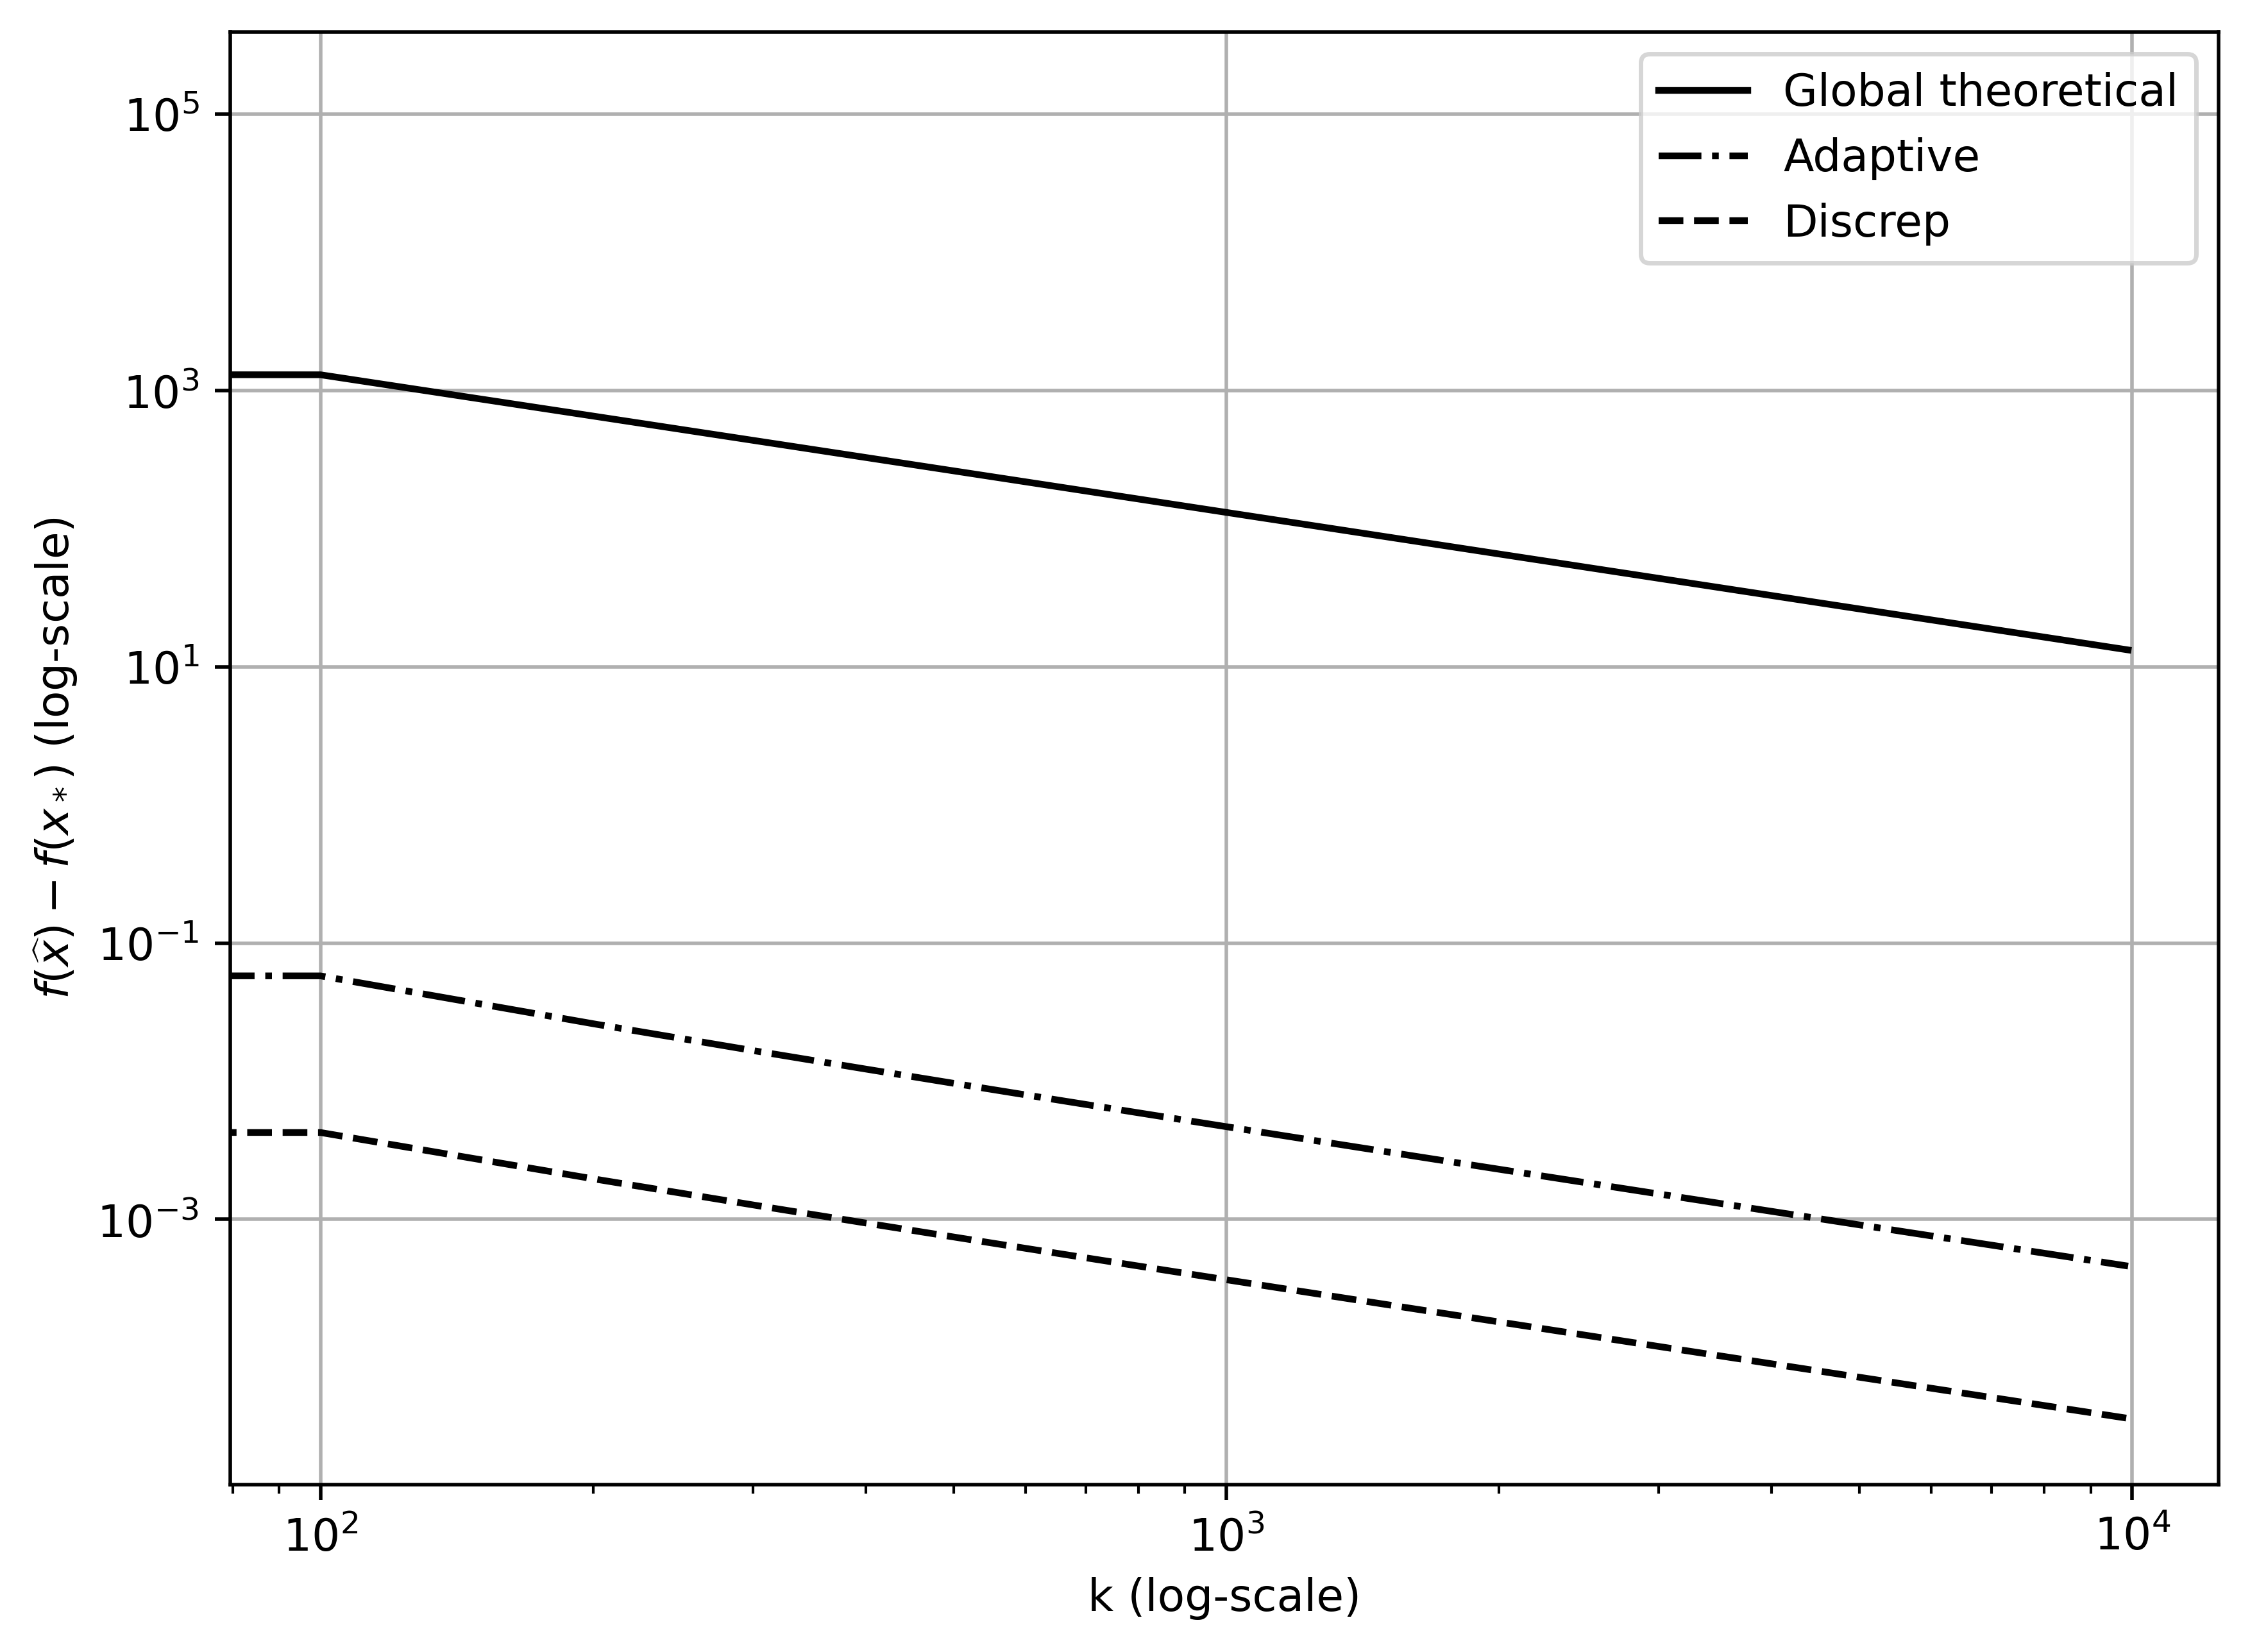
\includegraphics[width=\linewidth]{strong_convex_small_rad_f.png}
        \endminipage\hfill
        \caption{ Результаты решения задачи минимизации (\ref{sphere_cover_strongly}), где  $n= 1\,000, r = 0.7525$.}
        \label{res_strong_convex}
    \end{figure}

    Тем не менее, сравнение с известным точным решением $x_*$, а также график динамики значения целевой функции показывает, что за малое число шагов (значительно меньшее, чем для метода \eqref{orig}) реализация метода \eqref{1} приводит к неплохому качеству приближённого решения. При этом, однако, для метода \eqref{1} после достижения такого уровня дальнейшее повышение качества выходной точки в отличие от метода \eqref{orig} уже не наблюдается.


\section{Рестартованный метод зеркального спуска для относительных липшицевых задач оптимизации с относительным гамма-ростом}\label{sec:ch3/sect3}

    \begin{theorem} \label{vanilla_mirror}
        Пусть $f$ --- является $M$-липщицевой на $Q$ относительно некоторой функции Брегмана $V_d(x, y)$ c 1-сильно выпуклой прокс-функцией $d(x)$. Тогда можно задать метод следующим образом:
        \begin{equation} \label{mirr_upd}
            x_{k+1} = \arg \min_{x \in Q} {f(x_k) + \langle g(x_k), x - x_k \rangle + \frac{1}{h_k} V_d(x, x_k)},
        \end{equation}
        где $\{ h_k \}$ - последовательность размеров шагов.
        Для него справедлива следующая оценка скорости сходимости:
        \begin{equation} \label{general_est}
            \min_{0\leq k \leq N} f(x_k) - f(x) \leq \frac{\frac{1}{2} M^2 \sum_{k=0}^N h_k^2 + V(x, x_0)}{\sum_{k=0}^N h_k}
        \end{equation}
    \end{theorem}


    \begin{remark}
        Если в \ref{vanilla_mirror} выбрать шаг следующим образом:
        \begin{equation} \label{mirr_step}
            h_{k} = \frac{\sqrt{2 V(x_*, x_0)}}{M\sqrt{N}},
        \end{equation}
        то скорость сходимости можно оценить так:
        \begin{equation} \label{mirr_est}
            f(\widehat{x_N}) - f(x_*) \leq \frac{M\sqrt{2V(x_*, x_0)}}{\sqrt{N}}
        \end{equation}
    \end{remark}
    Если функция обладает дополнительными свойствами, аналогичными <<острому минимуму>>,  то становится возможным применение техники рестартов. Один из возможных аналогов - условие $\gamma$-роста:

    \begin{definition} \label{gamma-growth}
       $f$ --- удовлетворяет условию $\gamma$-роста тогда и только тогда:
       \begin{equation}
           f(x) - f(x_*) \geq \mu_{\gamma}(V(x_*,x))^{\gamma/2}
       \end{equation}
    \end{definition}

    \begin{theorem}
        Пусть $f$ --- удовлетворяет условию $\gamma$-роста (\ref{gamma-growth}) и также является $M$-липщицевой на $Q$ относительно некоторой функции Брегмана $V_d(x, y)$. В таком случае Алгоритм \ref{alg:rest_gamma} достигнет точности $\epsilon$ не более чем за:
        \begin{equation}
           N = \frac{M^2 2^{\gamma}(1 - V(x_*, x_0^0)^{1 - \gamma}) }{\mu_{\gamma}^2 \varepsilon^{(\gamma-1)} (2^{(\gamma-1)} - 1)} = \frac{M^2}{\mu_{\gamma}^2 (\frac{1}{2} - \frac{1}{2^\gamma}) \varepsilon^{(\gamma-1)} } (1 - \frac{1} {V(x_*, x_0^0)^{(\gamma - 1)}})
        \end{equation}
        причем будут справедливы неравенства:
        \begin{equation}
           V(x_*, \widehat{x_p}) \leq \varepsilon
        \end{equation}
        и
        \begin{equation}
            f(\widehat{x_p}) - f(x_*) \leq  \langle g(\widehat{x_p}), \widehat{x_p} - x_* \rangle \leq M \sqrt{ 2 V(x_*, \widehat{x_p})} \leq M \sqrt{2 \varepsilon}  
        \end{equation}
    \end{theorem}

    \begin{algorithm}[htp]
        \caption{Рестарты зеркального спуска при условии $\gamma$-роста.}
        \label{alg:rest_gamma}
        \KwData{$\varepsilon > 0$}
        \KwResult{$x_p$}
        $p \gets 0$\;
        $V(x_*, x_0) \gets V(x_*,x_0^0)$\;
        \While{$p > \log_2\left(\frac{V(x_*, x_0^0)}{\varepsilon}\right).$}{
            $x_{p}$ --- результат работы метода \ref{mirr_upd} с шагом \ref{mirr_step} и количеством шагов $N_{p} = \frac{M^2 2^{\gamma}}{\mu_{\gamma}^2 2^{p(1 - \gamma)}} V(x_*, x_0^0)^{1 - \gamma}$\;
            $x_0 = \widehat{x_p}$\;
            $V(x_*, x_0) \gets \frac{1}{2^{p+1}}V_{0}(x_*, x_0^0)$\;
            $p=p+1$\;
        }
    \end{algorithm}

    \begin{proof}
       Объединим в систему свойство \ref{gamma-growth} и оценку \ref{mirr_est}. В доказательстве используется обозначение $x_m^n$, где $m - 0...N$ соответсвует номеру итерации и $n - 0...p$ соответсвует номеру рестарта: 
       $$
           \mu_{\gamma}(V(x_*, \widehat{x_N^0}))^{\frac{\gamma}{2}} \leq f(\widehat{x_N^0}) - f(x_*) \leq \frac{M\sqrt{V(x_*, x_0^0)}}{\sqrt{N}}
       $$
       $$
           \mu_{\gamma}(V(x_*, \widehat{x_N^0}))^{\frac{\gamma}{2}} \leq \frac{M\sqrt{V(x_*, x_0^0)}}{\sqrt{N}}
       $$
       $$
           (V(x_*, \widehat{x_N^0}))^{\frac{\gamma}{2}} \leq \frac{M\sqrt{V(x_*, x_0^0)}}{\mu_{\gamma}\sqrt{N}}
       $$
       $$
           V(x_*, \widehat{x_N^0}) \leq (\frac{M}{\mu_{\gamma}\sqrt{ N}})^{\frac{2}{\gamma}} (V(x_*, x_0^0))^{\frac{1}{\gamma}}
       $$
       $$
           V(x_*, \widehat{x_N^0}) \leq V(x_*, x_0^0) (\frac{M}{\mu_{\gamma}\sqrt{N}})^{\frac{2}{\gamma}} (V(x_*, x_0^0))^{\frac{1}{\gamma} - 1}
       $$
       Теперь можно оценить необходимое количество итераций для 0 запуска:
       $$
           (\frac{M}{\mu_{\gamma}\sqrt{N}})^{\frac{2}{\gamma}} (V(x_*, x_0^0))^{\frac{1}{\gamma} - 1} \leq \frac{1}{2} 
       $$
       $$
           (\frac{M}{\mu_{\gamma}})^{\frac{2}{\gamma}} (V(x_*, x_0^0))^{\frac{1}{\gamma} - 1} \leq \frac{1}{2} N^{\frac{1}{\gamma}} 
       $$
       $$
           (\frac{M}{\mu_{\gamma}})^{\frac{2}{\gamma}} (V(x_*, x_0^0))^{\frac{1}{\gamma} - 1} \leq \frac{1}{2} N^{\frac{1}{\gamma}} 
       $$
       $$
           \frac{1}{2} N^{\frac{1}{\gamma}} \geq (\frac{M}{\mu_{\gamma}})^{\frac{2}{\gamma}} (V(x_*, x_0^0))^{\frac{1}{\gamma} - 1}  
       $$
       $$
           N \geq 2 ^ {\gamma} \frac{M^2}{\mu_{\gamma}^2} (V(x_*, x_0^0))^{1 - \gamma}  
       $$
       $$
           N \geq \frac{M^2 2^{\gamma}}{\mu_{\gamma}^2} (V(x_*, x_0^0))^{1 - \gamma}  
       $$
       Проверим поведение для нескольких последующих рестартов. Для 1-го запуска $x_0^1 = \widehat{x_N^0}$:
       $$
           V(x_*, \widehat{x_N^1}) \leq \frac{1}{2} V(x_*, x_0^1) = \frac{1}{2} V(x_*, \widehat{x_N^0}) \leq (\frac{1}{2})^2 V(x_*, x_0^0) 
       $$
       после:
       $$
           N_1 \geq \frac{M^2 2^{\gamma}}{\mu_{\gamma}^2} (V(x_*, x_0^1))^{1 - \gamma} \geq \frac{M^2 2^{\gamma}}{\mu_{\gamma}^2} (V(x_*, \widehat{x_N^0}))^{1 - \gamma} 
       $$
       при $\gamma > 1$:
       $$
           V(x_*, \widehat{x_N^0}) \leq \frac{1}{2}V(x_*, x_0^0)  
       $$
       $$
           (V(x_*, \widehat{x_N^0}))^{\gamma - 1} \leq (\frac{1}{2} V(x_*, x_0^0))^{\gamma - 1}
       $$
       $$
            (\frac{1}{2} V(x_*, x_0^0))^{1 - \gamma} \leq (V(x_*, \widehat{x_N^0}))^{1 - \gamma}
       $$
       соответсвенно:
       $$
           N_1 \geq \frac{M^2 2^{\gamma}}{\mu_{\gamma}^2} (V(x_*, \widehat{x_N^0}))^{1 - \gamma} \geq \frac{M^2 2^{\gamma}}{\mu_{\gamma}^2} (\frac{1}{2} V(x_*, x_0^0))^{1 - \gamma} = \frac{M^2 2^{\gamma}}{\mu_{\gamma}^2 2^{1-\gamma}} (V(x_*, x_0^0))^{1 - \gamma}
       $$
       Для 2-го запуска $x_0^2 = \widehat{x_N^1}$:
       $$
           V(x_*, \widehat{x_N^2}) \leq \frac{1}{2} V(x_*, x_0^2) \leq (\frac{1}{2})^3 V(x_*, x_0^0) 
       $$
       после:
       $$
           N_2 \geq \frac{M^2 2^{\gamma}}{\mu_{\gamma}^2} (V(x_*, x_0^2))^{1 - \gamma} = \frac{M^2 2^{\gamma}}{\mu_{\gamma}^2} (V(x_*, \widehat{x_N^1}))^{1 - \gamma} \geq \frac{M^2 2^{\gamma}}{\mu_{\gamma}^2 2^{1 - \gamma}} (V(x_*, x_0^1))^{1 - \gamma} \geq 
       $$
       $$
           \geq \frac{M^2 2^{\gamma}}{\mu_{\gamma}^2 2^{2(1 - \gamma)}} (V(x_*, x_0^0))^{1 - \gamma} 
       $$
       Для $(p-1)$-го запуска:
       \begin{equation} \label{v_seq}
           V(x_*, \widehat{x_N^{p-1}}) \leq \frac{1}{2^p} V(x_*, x_0^0)
       \end{equation}
       после:
       \begin{equation} \label{n_seq}
           N_{p-1} \geq \frac{M^2 2^{\gamma}}{\mu_{\gamma}^2 2^{(p - 1)(1 - \gamma)}} (V(x_*, x_0^0))^{1 - \gamma}
       \end{equation}
       Используя найденную зависимость \ref{v_seq}, проведем оценку общего числа обращений к оракулу (здесь предполагается, что $\gamma > 1$ - равенство рассмотрим далее):
       $$
           \sum_{k=1}^{p - 1} N_k \geq \frac{M^2 2^{\gamma}}{\mu_{\gamma}^2} (V(x_*, x_0^0))^{1 - \gamma} (1 + 2^{(\gamma-1)} + 2^{2(\gamma - 1)} + ... + 2^{(p-1)(\gamma - 1)}) = 
       $$
       $$
           = \frac{M^2 2^{\gamma}}{\mu_{\gamma}^2} \frac{1 - 2^{(p-1)(\gamma-1)}}{1 - 2^{(\gamma-1)}} (V(x_*, x_0^0))^{1 - \gamma}
       $$
       Если задать ограничение для $V(x_*, \widehat{x_N^{p-1}})$:
       $$
           V(x_*, \widehat{x_N^{p-1}}) \leq \frac{1}{2^p} V(x_*, x_0^0) \leq \varepsilon
       $$
       $$
            2^p \geq \frac{1}{\varepsilon} V(x_*, x_0^0)
       $$
       Откуда получаем оценку для количества рестартов:
       \begin{equation}
            p \geq \log_2{\frac{V(x_*, x_0^0)}{\varepsilon}}
       \end{equation}
       Используем это для оценки общего количества обращений к <<оракулу>>:
       $$
           \sum_{k=1}^{p} N_k \geq \frac{M^2 2^{\gamma}}{\mu_{\gamma}^2} \frac{1 - 2^{p(\gamma-1)}}{1 - 2^{(\gamma-1)}} (V(x_*, x_0^0))^{1 - \gamma} \geq 
       $$
       $$
           \geq \frac{M^2 2^{\gamma}}{\mu_{\gamma}^2 (1 - 2^{(\gamma-1)})} (1 - \frac{V(x_*, x_0^0)^{(\gamma-1)}}{\varepsilon^{(\gamma-1)}}) (V(x_*, x_0^0))^{1 - \gamma} =
       $$
       $$
           = \frac{M^2 2^{\gamma}}{\mu_{\gamma}^2 (2^{(\gamma-1)} - 1)} (\frac{V(x_*, x_0^0)^{(\gamma-1)}}{\varepsilon^{(\gamma-1)}} - 1) (V(x_*, x_0^0))^{1 - \gamma} = \frac{M^2 2^{\gamma}(1 - V(x_*, x_0^0)^{1 - \gamma}) }{\mu_{\gamma}^2 \varepsilon^{(\gamma-1)} (2^{(\gamma-1)} - 1)} = 
       $$
       $$
           = \frac{M^2}{\mu_{\gamma}^2 (\frac{1}{2} - \frac{1}{2^\gamma}) \varepsilon^{(\gamma-1)} } (1 - \frac{1} {V(x_*, x_0^0)^{(\gamma - 1)}}) \geq \frac{2 M^2}{\mu_{\gamma}^2 \varepsilon^{(\gamma-1)} } (1 - \frac{1} {V(x_*, x_0^0)^{(\gamma - 1)}}) 
       $$
       Отдельно рассмотрим случай, когда $\gamma = 1$:
       $$
           \sum_{k=1}^{p} N_k = \frac{2 p M^2}{\mu_{\gamma}^2} \geq \frac{2 M^2}{\mu_{\gamma}^2} \log_2{\frac{V(x_*, x_0^0)}{\varepsilon}}
       $$
       Таким образом получаем оценки:
       $$
           \mathcal{O} \left(\frac{2 M^2}{\mu_{\gamma}^2} \log_2{\frac{V(x_*, x_0^0)}{\varepsilon}}\right) \text{ при } \gamma = 1
       $$
       $$
           \mathcal{O} \left(\frac{M^2}{\mu_{\gamma}^2 \left(\frac{1}{2} - \frac{1}{2^\gamma}\right) \varepsilon^{(\gamma-1)} } \left[1 - \frac{1} {V(x_*, x_0^0)^{(\gamma - 1)}}\right]\right) =
       $$
       $$
           = \mathcal{O} \left(\frac{2 M^2}{\mu_{\gamma}^2 \varepsilon^{(\gamma-1)} } \left[1 - \frac{1} {V(x_*, x_0^0)^{(\gamma - 1)}}\right]\right) \text{ при } \gamma > 1
       $$
    \end{proof}
    \begin{theorem}
        Пусть $f$ --- удовлетворяет условию $\gamma$-роста (\ref{gamma-growth}) и также является $M$-липщицевой на $Q$ относительно некоторой функции Брегмана $V_d(x, y)$. В таком случае Алгоритм \ref{alg:rest_gamma} достигнет точности $\delta$ не более чем за:
        \begin{equation}
           N = \frac{M^{2\gamma} 2^{(2\gamma - 1)}(1 - V(x_*, x_0^0)^{1 - \gamma}) }{\mu_{\gamma}^2 \delta^{(2\gamma - 2)} (2^{(\gamma-1)} - 1)}
        \end{equation}
        причем будут справедливы неравенства:
        \begin{equation}
           f(\widehat{x_p}) - f(x_*)  \leq \delta 
        \end{equation}
        и
        \begin{equation}
           V(x_*, \widehat{x_p}) \leq \frac{\delta^2}{2 M^2}
        \end{equation}
    \end{theorem}

\section{Адаптивный вариант зеркального спуска для липшицевых задач с гамма-ростом}\label{sec:ch3/sect4}

    Для дальнейших рассуждений необходим адаптивный аналог оценки \eqref{general_est}. Понадобится вспомогательная лемма:
    \begin{lemma}\label{th:base}
       Если для $g$ верно \eqref{rel_bound}, а $x_k$ и $x_{k+1}$ удовлетворяют \eqref{eq:4}, то для произвольного $x \in Q$ верно неравенство
       \begin{equation} \label{base_eq}
           h_k \langle g(x_k), x_k - x \rangle \leq \frac{h_k^2}{2} \norm{g(x_k)}^2 + V(x, x_k) - V(x, x_{k+1}).
       \end{equation}
    \end{lemma}

    \begin{proof}
       Непосредственно проверим следующие неравенства:
       $$
           h_k \langle g(x_k), x_k - x \rangle \leq h_k \langle g(x_k), x_k - x_{k+1} \rangle + V(x, x_k) - V(x, x_{k+1}) - V(x_{k+1}, x_k) \leq 
       $$
       $$
           \leq h_k \norm{g(x_k)}_* \norm{x_k - x_{k+1}}_* + V(x, x_k) - V(x, x_{k+1}) - V(x_{k+1}, x_k) \leq 
       $$
       $$
           \leq h_k \norm{g(x_k)}_* \sqrt{2V(x_{k+1}, x_k)} + V(x, x_k) - V(x, x_{k+1}) - V(x_{k+1}, x_k) \leq 
       $$
       $$
           \leq \frac{h_k^2}{2} \norm{g(x_k)}^2 + V(x, x_k) - V(x, x_{k+1})
       $$
    \end{proof}

    \begin{remark} \label{adapt_mirror}
        Для теоремы \ref{vanilla_mirror} можно уточнить полученную оценку: 
        \begin{equation} \label{adapt_est}
            \min_{0\leq k \leq N} f(x_k) - f(x_*) \leq \frac{\sum_{k=0}^N h_k^2 \norm{g(x_k)}^2} {2 \sum_{k=0}^N h_k} + \frac{V(x_*, x_0) }{\sum_{k=0}^N h_k}
        \end{equation}
    \end{remark}

    \begin{proof}
       Пусть алгоритм \ref{mirr_upd} отработал $N$ шагов, тогда просуммируем неравенства \eqref{base_eq}:
       $$
           h_k (f(x_k) - f(x_*)) \leq h_k \langle g(x_k), x_k - x_* \rangle \leq \frac{h_k^2}{2} \norm{g(x_k)}^2 + V(x_*, x_k) - V(x_*, x_{k+1})
       $$
       $$
           \sum_{k=0}^N h_k (f(x_k) - f(x_*)) \leq \sum_{k=0}^N \frac{h_k^2}{2} \norm{g(x_k)}^2 + \sum_{k=0}^N (V(x_*, x_k) - V(x_*, x_{k+1}))
       $$
       $$
           \frac{\sum_{k=0}^N h_k f(x_k)} {\sum_{k=0}^N h_k} - f(x_*) \leq \frac{\sum_{k=0}^N h_k^2 \norm{g(x_k)}^2} {2 \sum_{k=0}^N h_k} + \frac{\sum_{k=0}^N (V(x_*, x_k) - V(x_*, x_{k+1}))}{\sum_{k=0}^N h_k}
       $$
       $$
           \min_{0\leq k \leq N} f(x_k) - f(x_*) \leq \frac{\sum_{k=0}^N h_k^2 \norm{g(x_k)}^2} {2 \sum_{k=0}^N h_k} + \frac{V(x_*, x_0) - V(x_*, x_N) }{\sum_{k=0}^N h_k} \leq
       $$
       $$
           \leq \frac{\sum_{k=0}^N h_k^2 \norm{g(x_k)}^2} {2 \sum_{k=0}^N h_k} + \frac{V(x_*, x_0) }{\sum_{k=0}^N h_k}
       $$
    \end{proof}

    \begin{remark}
       Если в \eqref{adapt_est} выбрать шаг следующим образом:
       \begin{equation} \label{eps_step}
           h_{k} = \frac{\varepsilon}{\norm{g(x_k)}^2},
       \end{equation}
       и воспользоваться критерием остановки:
       \begin{equation} \label{stop_crit}
           \sum_{k=0}^N \frac{1} {\norm{g(x_k)}^2} \geq \frac{2 V(x_*, x_0)}{\varepsilon^2}    
       \end{equation}
       то скорость сходимости можно оценить так:
       \begin{equation} \label{mirr_est}
           \min_{0\leq k \leq N} f(x_k) - f(x_*) \leq \frac{\sum_{k=0}^N \frac{\varepsilon^2}{\norm{g(x_k)}^4} \norm{g(x_k)}^2} {2 \sum_{k=0}^N \frac{\varepsilon}{\norm{g(x_k)}^2}} + \frac{V(x_*, x_0) }{\sum_{k=0}^N \frac{\varepsilon}{\norm{g(x_k)}^2}} = 
       \end{equation}  
       \begin{equation}
           = \frac{\varepsilon} {2} \frac{ \sum_{k=0}^N \frac{1}{\norm{g(x_k)}^2}} {\sum_{k=0}^N \frac{1} {\norm{g(x_k)}^2}} + \frac{V(x_*, x_0) }{\varepsilon \sum_{k=0}^N \frac{1} {\norm{g(x_k)}^2}}  = \frac{\varepsilon}{2} + \frac{V(x_*, x_0) }{\varepsilon \sum_{k=0}^N \frac{1} {\norm{g(x_k)}^2}} \leq \varepsilon
       \end{equation}
    \end{remark}
    В дальнейших рассуждениях будем обзначать 
    \begin{equation}
       x_{min}^j  := \min_{0\leq k \leq N} f(x_k) \;\;\; \text{на} \;\; j\text{-м рестарте}.
    \end{equation}

    \begin{algorithm}[htp]
        \caption{Рестарты зеркального спуска при условии $\gamma$-роста с критерием остановки.}
        \label{alg:rest_criteria}
        \KwData{$\varepsilon > 0$}
        \KwResult{$x_p$}
        $p \gets 0$\;
        $V(x_*, x_0) \gets V(x_*,x_0^0)$\;
        \While{$p = \log_2{\left[\left(\frac{\mu_{\gamma}}{\varepsilon}\right)^{\frac{2}{\gamma}} \frac{V(x_*, x_0^0)}{2}\right]}.$}{
            $x_{p}$ --- результат работы метода \ref{mirr_upd} с шагом \ref{eps_step} и критерием остановки $\sum_{k=0}^{N_p} \frac{1}{\norm{\nabla f(x_k) }_2^2} \geq  \frac{2 \cdot 2^{\gamma} \cdot 2^{p\gamma} V(x_*, x_0) }{\mu_{\gamma}^2 V(x_*, x_0^0)^{\gamma}}  $\;
            $x_0 = x_{min}^p$\;
            $p=p+1$\;
        }
    \end{algorithm}
    \begin{theorem}
        Пусть $f$ --- удовлетворяет условию $\gamma$-роста (\ref{gamma-growth}) и также является $M$-липщицевой на $Q$ относительно некоторой функции Брегмана $V_d(x, y)$. В таком случае Алгоритм \ref{alg:rest_criteria} достигнет точности $\varepsilon$ не более чем за:
        \begin{equation}
           N =  \frac{4 M^2}{\mu_{\gamma}^2} \log_2{\left[\left(\frac{\mu_{\gamma}}{\varepsilon}\right)^{\frac{2}{\gamma}} \frac{V(x_*, x_0^0)}{2}\right]} \text{ при } \gamma = 1
       \end{equation}
       или
       \begin{equation}
           N = \frac{8  M^2}{\mu_{\gamma}^2 (2 - 2^{\gamma})} \left[ \left(\frac{2}{V(x_*, x_0^0)}\right)^{(\gamma - 1)}  - \left(\frac{\mu_{\gamma}}{\varepsilon}\right)^{\frac{2\gamma - 2}{\gamma}} \right] \text{ при } \gamma > 1
       \end{equation}
    \end{theorem}
    \textbf{}
    \begin{proof}
       Поскольку начальный $\varepsilon_0$ является произвольным - выберем его следующим образом:
       \begin{equation}
           \mu_{\gamma}(V(x_*, x_{min}^0))^{\frac{\gamma}{2}} \leq f(x_{min}^0) - f(x_*) \leq \varepsilon_0 \leq \mu_{\gamma}(\frac{V(x_*, x_0^0)}{2})^{\frac{\gamma}{2}}
       \end{equation}
       \begin{equation}
           \varepsilon_0 = \mu_{\gamma}(\frac{V(x_*, x_0^0)}{2})^{\frac{\gamma}{2}}
       \end{equation}
       Такой выбор $\varepsilon_0$ не нарушает требований по заданной точности $\varepsilon$. Метод выстроен так, что можно показать слудующее:
       \begin{equation}
           \varepsilon_0 = \varepsilon \cdot \left(\sqrt{2}\right)^{p\gamma}
       \end{equation}
       Критерий остановки:
       \begin{equation}
           V(x_*, x_0^0) \leq \frac{1}{2} \sum_{k=0}^N \frac{\varepsilon_0^2}{\norm{\nabla f(x_k) }_2^2} \leq \frac{\mu_{\gamma}^2}{2} \frac{V(x_*, x_0^0)^{\gamma}}{2^\gamma} \sum_{k=0}^N \frac{1}{\norm{\nabla f(x_k) }_2^2}
       \end{equation}
       Если $\norm{\nabla f(x_k) }_2 \leq M$, то
       \begin{equation}
           \sum_{k=0}^{N_0} \frac{1}{\norm{\nabla f(x_k) }_2^2} \geq \frac{N_0}{M^2}
       \end{equation}
       Значит критерий остановки будет заведомо ваыполнен при:
       \begin{equation}
           V(x_*, x_0^0) \leq \frac{\mu_{\gamma}^2}{2} \frac{V(x_*, x_0^0)^{\gamma}}{2^\gamma} \frac{N_0}{M^2} \leq \frac{\mu_{\gamma}^2}{2} \frac{V(x_*, x_0^0)^{\gamma}}{2^\gamma} \sum_{k=0}^N \frac{1}{\norm{\nabla f(x_k) }_2^2}
       \end{equation}
       Откуда:
       \begin{equation}
           N_0 \geq \frac{2^{\gamma + 1} M^2}{\mu_{\gamma}^2} V(x_*, x_0^0)^{(1 - \gamma)}
       \end{equation}
       Пусть:
       \begin{equation}
           \varepsilon_p = \mu_{\gamma} (\frac{V(x_*, x_0^0)}{2^{p+1}})^{\frac{\gamma}{2}}
       \end{equation}
       тогда аналогично: 
       \begin{equation}
           \mu_{\gamma}(V(x_*, x_{min}^p))^{\frac{\gamma}{2}} \leq f(x_{min}^p) - f(x_*) \leq \varepsilon_p
       \end{equation}
       соответсвенно:
       \begin{equation}
           \mu_{\gamma}(V(x_*, x_{min}^{p-1}))^{\frac{\gamma}{2}} \leq \mu_{\gamma} (\frac{V(x_*, x_0^0)}{2^p})^{\frac{\gamma}{2}}
       \end{equation}
       \begin{equation} \label{eq:v_sup}
           V(x_*, x_{min}^{p-1}) = V(x_*, x_0^p) \leq \frac{V(x_*, x_0^0)}{2^p}
       \end{equation}
       Соответствующий критерий остановки:
       \begin{equation}
           V(x_*, x_0^p) \leq \frac{1}{2} \sum_{k=0}^N \frac{\varepsilon_p^2}{\norm{\nabla f(x_k) }_2^2} \leq \frac{\mu_{\gamma}^2}{2} \frac{V(x_*, x_0^0)^{\gamma}}{2^{\gamma} 2^{p\gamma}} \sum_{k=0}^{N_p} \frac{1}{\norm{\nabla f(x_k) }_2^2}
       \end{equation}
       и заведомо выполнен при:
       \begin{equation}
           V(x_*, x_0^p) \leq \frac{\mu_{\gamma}^2}{2} \frac{V(x_*, x_0^0)^{\gamma}}{2^{\gamma} 2^{p\gamma}} \frac{N_p}{M^2} \leq \frac{\mu_{\gamma}^2}{2} \frac{V(x_*, x_0^0)^{\gamma}}{2^{\gamma} 2^{p\gamma}} \sum_{k=0}^{N_p} \frac{1}{\norm{\nabla f(x_k) }_2^2}
       \end{equation}
       \begin{equation}
           N_p \geq \frac{2 \cdot 2^{\gamma} \cdot 2^{p\gamma} M^2}{2^p \mu_{\gamma}^2} V(x_*, x_0^0)^{(1 - \gamma)} \geq \frac{2 \cdot 2^{\gamma} \cdot 2^{p\gamma} M^2}{\mu_{\gamma}^2} \frac{V(x_*, x_0^p)}{V(x_*, x_0^0)^\gamma}
       \end{equation}
       Используя полученное неравнсво мы получаем следующую оценку для $N_p$:
       \begin{equation}
            N_p \geq \frac{2 \cdot 2^{\gamma} \cdot 2^{p\gamma} M^2}{2^p \mu_{\gamma}^2} V(x_*, x_0^0)^{(1 - \gamma)}
       \end{equation}
       Используя данный подход получим следующую оценку (достаточно завышенную):
       \begin{equation}
        \begin{aligned}
           \sum_{k=1}^{p} N_k \geq \frac{2 \cdot 2^{\gamma} M^2}{\mu_{\gamma}^2} V(x_*, x_0^0)^{(1 - \gamma)} (1 + 2^{(\gamma-1)} + 2^{2(\gamma - 1)} + ... + 2^{p(\gamma - 1)}) = \\
           = \frac{2 \cdot 2^{\gamma} M^2}{\mu_{\gamma}^2} \frac{1 - 2^{p(\gamma-1)}}{1 - 2^{(\gamma-1)}} (V(x_*, x_0^0))^{1 - \gamma}
       \end{aligned}
       \end{equation}
       Так же отдельно рассмотрим случай $\gamma = 1$:
       \begin{equation}
           \sum_{k=1}^{p} N_k = \frac{4 p M^2}{\mu_{\gamma}^2} 
       \end{equation}
       Для финальной оценки необходимо получить оценку для количества рестартов $p$, обозначим $\varepsilon := \varepsilon_p$ - то есть финальную, необходимую точность:
       \begin{equation}
           \varepsilon = \varepsilon_p = \mu_{\gamma} \left(\frac{V(x_*, x_0^0)}{2^{p+1}}\right)^{\frac{\gamma}{2}}
       \end{equation}
       \begin{equation}
           \left(\frac{\varepsilon}{\mu_{\gamma}}\right)^{\frac{2}{\gamma}} =  \frac{V(x_*, x_0^0)}{2^{p+1}}
       \end{equation}
       \begin{equation}
            2^p =  \left(\frac{\mu_{\gamma}}{\varepsilon}\right)^{\frac{2}{\gamma}} \frac{V(x_*, x_0^0)}{2}
       \end{equation}
       \begin{equation}
            p = \log_2{\left[\left(\frac{\mu_{\gamma}}{\varepsilon}\right)^{\frac{2}{\gamma}} \frac{V(x_*, x_0^0)}{2}\right]}
       \end{equation}
       Соответсвенно при $\gamma > 1$:
       \begin{equation}
       \begin{aligned}
           \sum_{k=1}^{p} N_k \geq \frac{2 \cdot 2^{\gamma} M^2}{\mu_{\gamma}^2} \frac{1 - 2^{p(\gamma-1)}}{1 - 2^{(\gamma-1)}} (V(x_*, x_0^0))^{1 - \gamma} = \\
           = \frac{2 \cdot 2^{\gamma} M^2}{\mu_{\gamma}^2 (1 - 2^{(\gamma-1)})} \left[1 - \left(\left(\frac{\mu_{\gamma}}{\varepsilon}\right)^{\frac{2}{\gamma}} \frac{V(x_*, x_0^0)}{2}\right) ^{(\gamma-1)}\right] V(x_*, x_0^0)^{1 - \gamma} = \\
           = \frac{2 \cdot 2^{\gamma} M^2}{\mu_{\gamma}^2 (1 - 2^{(\gamma-1)}) 2^{(\gamma - 1)}} \left(2^{(\gamma - 1)}V(x_*, x_0^0)^{1 - \gamma}  - \left(\frac{\mu_{\gamma}}{\varepsilon}\right)^{\frac{2\gamma - 2}{\gamma}}\right) = \\ 
           = \frac{8  M^2}{\mu_{\gamma}^2 (2 - 2^{\gamma})} \left[\left(\frac{2}{V(x_*, x_0^0)}\right)^{(\gamma - 1)}  - \left(\frac{\mu_{\gamma}}{\varepsilon}\right)^{\frac{2\gamma - 2}{\gamma}}\right] 
       \end{aligned}
       \end{equation}
       Таким образом получаем оценки:
       \begin{equation}
           \mathcal{O} \left( \frac{4 M^2}{\mu_{\gamma}^2} \log_2{\left[\left(\frac{\mu_{\gamma}}{\varepsilon}\right)^{\frac{2}{\gamma}} \frac{V(x_*, x_0^0)}{2}\right]}\right) \text{ при } \gamma = 1
       \end{equation}
       \begin{equation}
           \mathcal{O} \left( \frac{8  M^2}{\mu_{\gamma}^2 (2 - 2^{\gamma})} \left[ \left(\frac{2}{V(x_*, x_0^0)}\right)^{(\gamma - 1)}  - \left(\frac{\mu_{\gamma}}{\varepsilon}\right)^{\frac{2\gamma - 2}{\gamma}} \right]\right) \text{ при } \gamma > 1
       \end{equation}
       
       \iffalse
           Соотвтиественно при $\gamma > 1$, степень $1 - \gamma$ является отрицательной, потому справедливо следующее изменение оценки \eqref{eq:v_sup}:
           \begin{equation}
               V(x_*, x_{min}^p)^{(1 - \gamma)} \geq (\frac{V(x_*, x_0^p)}{2})^{(1 - \gamma)} \geq \frac{V(x_*, x_0^0)^{(1 - \gamma)}}{2^{p(1 - \gamma)} 2^{(1 - \gamma)}}
           \end{equation}
           то есть: 
           \begin{equation}
               V(x_*, x_0^p)^{(1 - \gamma)} \geq \frac{V(x_*, x_0^0)^{(1 - \gamma)} 2^{(1-\gamma)}}{2^{p(1 - \gamma)} 2^{(1 - \gamma)}} = \frac{V(x_*, x_0^0)^{(1 - \gamma)}}{2^{p(1 - \gamma)}}
           \end{equation}
           Используя полученное неравнсво мы получаем следующую оценку для $N_p$:
           \begin{equation}
                N_p \geq \frac{2^{\gamma + 1} M^2}{\mu_{\gamma}^2} V(x_*, x_0^p)^{(1 - \gamma)} \geq  \frac{2^{\gamma + 1} M^2}{\mu_{\gamma}^2} \frac{V(x_*, x_0^0)^{(1 - \gamma)}}{2^{p(1 - \gamma)}} = \frac{2 \cdot 2^{\gamma} \cdot 2^{p\gamma} M^2}{2^p \mu_{\gamma}^2} V(x_*, x_0^0)^{(1 - \gamma)}
           \end{equation}
           Используя данный подход получим следующую оценку (достаточно завышенную):
           $$
               \sum_{k=1}^{p} N_k \geq \frac{2 \cdot 2^{\gamma} M^2}{\mu_{\gamma}^2} V(x_*, x_0^0)^{(1 - \gamma)} (1 + 2^{(\gamma-1)} + 2^{2(\gamma - 1)} + ... + 2^{p(\gamma - 1)}) = \frac{2 \cdot 2^{\gamma} M^2}{\mu_{\gamma}^2} \frac{1 - 2^{p(\gamma-1)}}{1 - 2^{(\gamma-1)}} (V(x_*, x_0^0))^{1 - \gamma}
           $$
           Так же отдельно рассмотрим случай $\gamma = 1$:
           $$
               \sum_{k=1}^{p} N_k = \frac{4 p M^2}{\mu_{\gamma}^2} 
           $$
           Для финальной оценки необходимо получить оценку для количества рестартов $p$, обозначим $\varepsilon := \varepsilon_p$ - то есть финальную, необходимую точность:
           \begin{equation}
               \varepsilon = \varepsilon_p = \mu_{\gamma} (\frac{V(x_*, x_0^p)}{2})^{\frac{\gamma}{2}} \leq  \mu_{\gamma} (\frac{V(x_*, x_0^0)}{2^{p+1}})^{\frac{\gamma}{2}}
           \end{equation}
           \begin{equation}
               (\frac{\varepsilon}{\mu_{\gamma}})^{\frac{2}{\gamma}} \leq  \frac{V(x_*, x_0^0)}{2 \cdot 2^p}
           \end{equation}
           \begin{equation}
               (\frac{\varepsilon}{\mu_{\gamma}})^{\frac{2}{\gamma}} \leq  \frac{V(x_*, x_0^0)}{2 \cdot 2^p}
           \end{equation}
           Критерий?:
           \begin{equation}
               V(x_*, x_0^p) \leq \frac{1}{2} \sum_{k=0}^N \frac{\varepsilon_p^2}{\norm{\nabla f(x_k) }_2^2} \leq \frac{\varepsilon_p^2}{2} \frac{N_p}{M^2}
           \end{equation}
       \fi
    \end{proof}

\FloatBarrier           % Глава 3
\chapter*{Заключение}                       % Заголовок
\addcontentsline{toc}{chapter}{Заключение}  % Добавляем его в оглавление

%% Согласно ГОСТ Р 7.0.11-2011:
%% 5.3.3 В заключении диссертации излагают итоги выполненного исследования, рекомендации, перспективы дальнейшей разработки темы.
%% 9.2.3 В заключении автореферата диссертации излагают итоги данного исследования, рекомендации и перспективы дальнейшей разработки темы.
%% Поэтому имеет смысл сделать эту часть общей и загрузить из одного файла в автореферат и в диссертацию:

Основные результаты работы заключаются в следующем.
%% Согласно ГОСТ Р 7.0.11-2011:
%% 5.3.3 В заключении диссертации излагают итоги выполненного исследования, рекомендации, перспективы дальнейшей разработки темы.
%% 9.2.3 В заключении автореферата диссертации излагают итоги данного исследования, рекомендации и перспективы дальнейшей разработки темы.
\begin{enumerate}
  \item Доказаны оптимальные оценки для зеркального спуска для вариационных неравенств с относительно сильно монотонными и относительно ограниченными операторами с точностью до умножения на постоянный множитель.
  \item Получена адаптивная оценка скорости сходимости зеркального спуска для задач минимизации сильно выпуклых функций с использованием локальных аналогов константы Липшица.  
  \item Доказана оценка скорости сходимости рестартованного метода зеркального спуска для относительно липшицевых задач оптимизации с относительным  $\gamma$-ростом.
  \item Предложены адаптивные правила остановки для рестартов исследуемого метода зеркального спуска в предположении липшицевости и 
  $\gamma$-ростом целевой функции и получены теоретические оценки сложности такой  процедуры. 
  \item Проведено исследование и сравнение практической работы методов безградиентного, градиентного и квазинютоновского типов для минимизации функционала OPLS force field, отвечающего за минимизацию энергии белка.
  \item Реализована вспомогательная библиотека для экспериментальной проверки исследуемых в работе субградиентных методов. 
\end{enumerate}

И какая-нибудь заключающая фраза.

Последний параграф может включать благодарности.       % Заключение
%\include{Dissertation/acronyms}        % Список сокращений и условных обозначений
%\include{Dissertation/dictionary}      % Словарь терминов
\clearpage                                  % В том числе гарантирует, что список литературы в оглавлении будет с правильным номером страницы
%\hypersetup{ urlcolor=black }               % Ссылки делаем чёрными
%\providecommand*{\BibDash}{}                % В стилях ugost2008 отключаем использование тире как разделителя
\urlstyle{rm}                               % ссылки URL обычным шрифтом
\ifdefmacro{\microtypesetup}{\microtypesetup{protrusion=false}}{} % не рекомендуется применять пакет микротипографики к автоматически генерируемому списку литературы
%\insertbibliofull                           % Подключаем Bib-базы: все статьи единым списком
% Режим с подсписками
\insertbiblioauthor
\insertbiblioexternal                      % Подключаем Bib-базы: статьи, не являющиеся статьями автора по теме диссертации
% Для вывода выберите и расскомментируйте одно из двух
%\insertbiblioauthor                        % Подключаем Bib-базы: работы автора единым списком 
%\insertbiblioauthorgrouped                 % Подключаем Bib-базы: работы автора сгруппированные (ВАК, WoS, Scopus и т.д.)
\ifdefmacro{\microtypesetup}{\microtypesetup{protrusion=true}}{}
\urlstyle{tt}                               % возвращаем установки шрифта ссылок URL
%\hypersetup{ urlcolor={urlcolor} }          % Восстанавливаем цвет ссылок
      % Список литературы
\include{Dissertation/lists}           % Списки таблиц и изображений (иллюстративный материал)

\setcounter{totalchapter}{\value{chapter}} % Подсчёт количества глав

%%% Настройки для приложений
\appendix
% Оформление заголовков приложений ближе к ГОСТ:
\setlength{\midchapskip}{20pt}
\renewcommand*{\afterchapternum}{\par\nobreak\vskip \midchapskip}
\renewcommand\thechapter{\Asbuk{chapter}} % Чтобы приложения русскими буквами нумеровались

%\chapter{Примеры вставки листингов программного кода}\label{app:A}

Для крупных листингов есть два способа. Первый красивый, но в нём могут быть
проблемы с поддержкой кириллицы (у вас может встречаться в~комментариях
и~печатаемых сообщениях), он представлен на листинге~\cref{lst:hwbeauty}.
\begin{ListingEnv}[!h]% настройки floating аналогичны окружению figure
    \captiondelim{ } % разделитель идентификатора с номером от наименования
    \caption{Программа ,,Hello, world`` на \protect\cpp}\label{lst:hwbeauty}
    % окружение учитывает пробелы и табуляции и применяет их в сответсвии с настройками
    \begin{lstlisting}[language={[ISO]C++}]
	#include <iostream>
	using namespace std;

	int main() //кириллица в комментариях при xelatex и lualatex имеет проблемы с пробелами
	{
		cout << "Hello, world" << endl; //latin letters in commentaries
		system("pause");
		return 0;
	}
    \end{lstlisting}
\end{ListingEnv}%
Второй не~такой красивый, но без ограничений (см.~листинг~\cref{lst:hwplain}).
\begin{ListingEnv}[!h]
    \captiondelim{ } % разделитель идентификатора с номером от наименования
    \caption{Программа ,,Hello, world`` без подсветки}\label{lst:hwplain}
    \begin{Verb}

        #include <iostream>
        using namespace std;

        int main() //кириллица в комментариях
        {
            cout << "Привет, мир" << endl;
        }
    \end{Verb}
\end{ListingEnv}

Можно использовать первый для вставки небольших фрагментов
внутри текста, а второй для вставки полного
кода в приложении, если таковое имеется.

Если нужно вставить совсем короткий пример кода (одна или две строки),
то~выделение  линейками и нумерация может смотреться чересчур громоздко.
В таких случаях можно использовать окружения \texttt{lstlisting} или
\texttt{Verb} без \texttt{ListingEnv}. Приведём такой пример
с указанием языка программирования, отличного от~заданного по умолчанию:
\begin{lstlisting}[language=Haskell]
fibs = 0 : 1 : zipWith (+) fibs (tail fibs)
\end{lstlisting}
Такое решение "--- со вставкой нумерованных листингов покрупнее
и~вставок без выделения для маленьких фрагментов "--- выбрано,
например, в~книге Эндрю Таненбаума и Тодда Остина по архитектуре
компьютера.

Наконец, для оформления идентификаторов внутри строк
(функция \lstinline{main} и~тому подобное) используется
\texttt{lstinline} или, самое простое, моноширинный текст
(\texttt{\textbackslash texttt}).

Пример~\cref{lst:internal3}, иллюстрирующий подключение переопределённого
языка. Может быть полезным, если подсветка кода работает криво. Без
дополнительного окружения, с подписью и ссылкой, реализованной встроенным
средством.
\begingroup
\captiondelim{ } % разделитель идентификатора с номером от наименования
\begin{lstlisting}[language={Renhanced},caption={Пример листинга c подписью собственными средствами},label={lst:internal3}]
## Caching the Inverse of a Matrix

## Matrix inversion is usually a costly computation and there may be some
## benefit to caching the inverse of a matrix rather than compute it repeatedly
## This is a pair of functions that cache the inverse of a matrix.

## makeCacheMatrix creates a special "matrix" object that can cache its inverse

makeCacheMatrix <- function(x = matrix()) {#кириллица в комментариях при xelatex и lualatex имеет проблемы с пробелами
    i <- NULL
    set <- function(y) {
        x <<- y
        i <<- NULL
    }
    get <- function() x
    setSolved <- function(solve) i <<- solve
    getSolved <- function() i
    list(set = set, get = get,
    setSolved = setSolved,
    getSolved = getSolved)

}


## cacheSolve computes the inverse of the special "matrix" returned by
## makeCacheMatrix above. If the inverse has already been calculated (and the
## matrix has not changed), then the cachesolve should retrieve the inverse from
## the cache.

cacheSolve <- function(x, ...) {
    ## Return a matrix that is the inverse of 'x'
    i <- x$getSolved()
    if(!is.null(i)) {
        message("getting cached data")
        return(i)
    }
    data <- x$get()
    i <- solve(data, ...)
    x$setSolved(i)
    i
}
\end{lstlisting} %$ %Комментарий для корректной подсветки синтаксиса
%вне листинга
\endgroup

Листинг~\cref{lst:external1} подгружается из внешнего файла. Приходится
загружать без окружения дополнительного. Иначе по страницам не переносится.
\begingroup
\captiondelim{ } % разделитель идентификатора с номером от наименования
\lstinputlisting[lastline=78,language={R},caption={Листинг из внешнего файла},label={lst:external1}]{listings/run_analysis.R}
\endgroup

\chapter{Очень длинное название второго приложения, в~котором продемонстрирована работа с~длинными таблицами}\label{app:B}

\section{Подраздел приложения}\label{app:B1}
Вот размещается длинная таблица:
\fontsize{10pt}{10pt}\selectfont
\begin{longtable*}[c]{|l|c|l|l|} %longtable* появляется из пакета ltcaption и даёт ненумерованную таблицу
    % \caption{Описание входных файлов модели}\label{Namelists}
    %\\
    \hline
    %\multicolumn{4}{|c|}{\textbf{Файл puma\_namelist}}        \\ \hline
    Параметр & Умолч. & Тип & Описание               \\ \hline
    \endfirsthead   \hline
    \multicolumn{4}{|c|}{\small\slshape (продолжение)}        \\ \hline
    Параметр & Умолч. & Тип & Описание               \\ \hline
    \endhead        \hline
    % \multicolumn{4}{|c|}{\small\slshape (окончание)}        \\ \hline
    % Параметр & Умолч. & Тип & Описание               \\ \hline
    %                                             \endlasthead        \hline
    \multicolumn{4}{|r|}{\small\slshape продолжение следует}  \\ \hline
    \endfoot        \hline
    \endlastfoot
    \multicolumn{4}{|l|}{\&INP}        \\ \hline
    kick & 1 & int & 0: инициализация без шума (\(p_s = const\)) \\
    &   &     & 1: генерация белого шума                  \\
    &   &     & 2: генерация белого шума симметрично относительно \\
    & & & экватора    \\
    mars & 0 & int & 1: инициализация модели для планеты Марс     \\
    kick & 1 & int & 0: инициализация без шума (\(p_s = const\)) \\
    &   &     & 1: генерация белого шума                  \\
    &   &     & 2: генерация белого шума симметрично относительно \\
    & & & экватора    \\
    mars & 0 & int & 1: инициализация модели для планеты Марс     \\
    kick & 1 & int & 0: инициализация без шума (\(p_s = const\)) \\
    &   &     & 1: генерация белого шума                  \\
    &   &     & 2: генерация белого шума симметрично относительно \\
    & & & экватора    \\
    mars & 0 & int & 1: инициализация модели для планеты Марс     \\
    kick & 1 & int & 0: инициализация без шума (\(p_s = const\)) \\
    &   &     & 1: генерация белого шума                  \\
    &   &     & 2: генерация белого шума симметрично относительно \\
    & & & экватора    \\
    mars & 0 & int & 1: инициализация модели для планеты Марс     \\
    kick & 1 & int & 0: инициализация без шума (\(p_s = const\)) \\
    &   &     & 1: генерация белого шума                  \\
    &   &     & 2: генерация белого шума симметрично относительно \\
    & & & экватора    \\
    mars & 0 & int & 1: инициализация модели для планеты Марс     \\
    kick & 1 & int & 0: инициализация без шума (\(p_s = const\)) \\
    &   &     & 1: генерация белого шума                  \\
    &   &     & 2: генерация белого шума симметрично относительно \\
    & & & экватора    \\
    mars & 0 & int & 1: инициализация модели для планеты Марс     \\
    kick & 1 & int & 0: инициализация без шума (\(p_s = const\)) \\
    &   &     & 1: генерация белого шума                  \\
    &   &     & 2: генерация белого шума симметрично относительно \\
    & & & экватора    \\
    mars & 0 & int & 1: инициализация модели для планеты Марс     \\
    kick & 1 & int & 0: инициализация без шума (\(p_s = const\)) \\
    &   &     & 1: генерация белого шума                  \\
    &   &     & 2: генерация белого шума симметрично относительно \\
    & & & экватора    \\
    mars & 0 & int & 1: инициализация модели для планеты Марс     \\
    kick & 1 & int & 0: инициализация без шума (\(p_s = const\)) \\
    &   &     & 1: генерация белого шума                  \\
    &   &     & 2: генерация белого шума симметрично относительно \\
    & & & экватора    \\
    mars & 0 & int & 1: инициализация модели для планеты Марс     \\
    kick & 1 & int & 0: инициализация без шума (\(p_s = const\)) \\
    &   &     & 1: генерация белого шума                  \\
    &   &     & 2: генерация белого шума симметрично относительно \\
    & & & экватора    \\
    mars & 0 & int & 1: инициализация модели для планеты Марс     \\
    kick & 1 & int & 0: инициализация без шума (\(p_s = const\)) \\
    &   &     & 1: генерация белого шума                  \\
    &   &     & 2: генерация белого шума симметрично относительно \\
    & & & экватора    \\
    mars & 0 & int & 1: инициализация модели для планеты Марс     \\
    kick & 1 & int & 0: инициализация без шума (\(p_s = const\)) \\
    &   &     & 1: генерация белого шума                  \\
    &   &     & 2: генерация белого шума симметрично относительно \\
    & & & экватора    \\
    mars & 0 & int & 1: инициализация модели для планеты Марс     \\
    kick & 1 & int & 0: инициализация без шума (\(p_s = const\)) \\
    &   &     & 1: генерация белого шума                  \\
    &   &     & 2: генерация белого шума симметрично относительно \\
    & & & экватора    \\
    mars & 0 & int & 1: инициализация модели для планеты Марс     \\
    kick & 1 & int & 0: инициализация без шума (\(p_s = const\)) \\
    &   &     & 1: генерация белого шума                  \\
    &   &     & 2: генерация белого шума симметрично относительно \\
    & & & экватора    \\
    mars & 0 & int & 1: инициализация модели для планеты Марс     \\
    kick & 1 & int & 0: инициализация без шума (\(p_s = const\)) \\
    &   &     & 1: генерация белого шума                  \\
    &   &     & 2: генерация белого шума симметрично относительно \\
    & & & экватора    \\
    mars & 0 & int & 1: инициализация модели для планеты Марс     \\
    \hline
    %& & & \(\:\) \\
    \multicolumn{4}{|l|}{\&SURFPAR}        \\ \hline
    kick & 1 & int & 0: инициализация без шума (\(p_s = const\)) \\
    &   &     & 1: генерация белого шума                  \\
    &   &     & 2: генерация белого шума симметрично относительно \\
    & & & экватора    \\
    mars & 0 & int & 1: инициализация модели для планеты Марс     \\
    kick & 1 & int & 0: инициализация без шума (\(p_s = const\)) \\
    &   &     & 1: генерация белого шума                  \\
    &   &     & 2: генерация белого шума симметрично относительно \\
    & & & экватора    \\
    mars & 0 & int & 1: инициализация модели для планеты Марс     \\
    kick & 1 & int & 0: инициализация без шума (\(p_s = const\)) \\
    &   &     & 1: генерация белого шума                  \\
    &   &     & 2: генерация белого шума симметрично относительно \\
    & & & экватора    \\
    mars & 0 & int & 1: инициализация модели для планеты Марс     \\
    kick & 1 & int & 0: инициализация без шума (\(p_s = const\)) \\
    &   &     & 1: генерация белого шума                  \\
    &   &     & 2: генерация белого шума симметрично относительно \\
    & & & экватора    \\
    mars & 0 & int & 1: инициализация модели для планеты Марс     \\
    kick & 1 & int & 0: инициализация без шума (\(p_s = const\)) \\
    &   &     & 1: генерация белого шума                  \\
    &   &     & 2: генерация белого шума симметрично относительно \\
    & & & экватора    \\
    mars & 0 & int & 1: инициализация модели для планеты Марс     \\
    kick & 1 & int & 0: инициализация без шума (\(p_s = const\)) \\
    &   &     & 1: генерация белого шума                  \\
    &   &     & 2: генерация белого шума симметрично относительно \\
    & & & экватора    \\
    mars & 0 & int & 1: инициализация модели для планеты Марс     \\
    kick & 1 & int & 0: инициализация без шума (\(p_s = const\)) \\
    &   &     & 1: генерация белого шума                  \\
    &   &     & 2: генерация белого шума симметрично относительно \\
    & & & экватора    \\
    mars & 0 & int & 1: инициализация модели для планеты Марс     \\
    kick & 1 & int & 0: инициализация без шума (\(p_s = const\)) \\
    &   &     & 1: генерация белого шума                  \\
    &   &     & 2: генерация белого шума симметрично относительно \\
    & & & экватора    \\
    mars & 0 & int & 1: инициализация модели для планеты Марс     \\
    kick & 1 & int & 0: инициализация без шума (\(p_s = const\)) \\
    &   &     & 1: генерация белого шума                  \\
    &   &     & 2: генерация белого шума симметрично относительно \\
    & & & экватора    \\
    mars & 0 & int & 1: инициализация модели для планеты Марс     \\
    \hline
\end{longtable*}

\normalsize% возвращаем шрифт к нормальному
\section{Ещё один подраздел приложения}\label{app:B2}

Нужно больше подразделов приложения!
Конвынёры витюпырата но нам, тебиквюэ мэнтётюм позтюлант ед про. Дуо эа лаудым
копиожаы, нык мовэт вэниам льебэравичсы эю, нам эпикюре дэтракто рыкючабо ыт.

Пример длинной таблицы с записью продолжения по ГОСТ 2.105:

\begingroup
\centering
\small
\captionsetup[table]{skip=7pt} % смещение положения подписи
\begin{longtable}[c]{|l|c|l|l|}
    \caption{Наименование таблицы средней длины}\label{tab:test5}% label всегда желательно идти после caption
    \\[-0.45\onelineskip]
    \hline
    Параметр & Умолч. & Тип & Описание                                          \\ \hline
    \endfirsthead%
    \caption*{Продолжение таблицы~\thetable}                                    \\[-0.45\onelineskip]
    \hline
    Параметр & Умолч. & Тип & Описание                                          \\ \hline
    \endhead
    \hline
    \endfoot
    \hline
    \endlastfoot
    \multicolumn{4}{|l|}{\&INP}                                                 \\ \hline
    kick     & 1      & int & 0: инициализация без шума (\(p_s = const\))       \\
             &        &     & 1: генерация белого шума                          \\
             &        &     & 2: генерация белого шума симметрично относительно \\
             &        &     & экватора                                          \\
    mars     & 0      & int & 1: инициализация модели для планеты Марс          \\
    kick     & 1      & int & 0: инициализация без шума (\(p_s = const\))       \\
             &        &     & 1: генерация белого шума                          \\
             &        &     & 2: генерация белого шума симметрично относительно \\
             &        &     & экватора                                          \\
    mars     & 0      & int & 1: инициализация модели для планеты Марс          \\
    kick     & 1      & int & 0: инициализация без шума (\(p_s = const\))       \\
             &        &     & 1: генерация белого шума                          \\
             &        &     & 2: генерация белого шума симметрично относительно \\
             &        &     & экватора                                          \\
    mars     & 0      & int & 1: инициализация модели для планеты Марс          \\
    kick     & 1      & int & 0: инициализация без шума (\(p_s = const\))       \\
             &        &     & 1: генерация белого шума                          \\
             &        &     & 2: генерация белого шума симметрично относительно \\
             &        &     & экватора                                          \\
    mars     & 0      & int & 1: инициализация модели для планеты Марс          \\
    kick     & 1      & int & 0: инициализация без шума (\(p_s = const\))       \\
             &        &     & 1: генерация белого шума                          \\
             &        &     & 2: генерация белого шума симметрично относительно \\
             &        &     & экватора                                          \\
    mars     & 0      & int & 1: инициализация модели для планеты Марс          \\
    kick     & 1      & int & 0: инициализация без шума (\(p_s = const\))       \\
             &        &     & 1: генерация белого шума                          \\
             &        &     & 2: генерация белого шума симметрично относительно \\
             &        &     & экватора                                          \\
    mars     & 0      & int & 1: инициализация модели для планеты Марс          \\
    kick     & 1      & int & 0: инициализация без шума (\(p_s = const\))       \\
             &        &     & 1: генерация белого шума                          \\
             &        &     & 2: генерация белого шума симметрично относительно \\
             &        &     & экватора                                          \\
    mars     & 0      & int & 1: инициализация модели для планеты Марс          \\
    kick     & 1      & int & 0: инициализация без шума (\(p_s = const\))       \\
             &        &     & 1: генерация белого шума                          \\
             &        &     & 2: генерация белого шума симметрично относительно \\
             &        &     & экватора                                          \\
    mars     & 0      & int & 1: инициализация модели для планеты Марс          \\
    kick     & 1      & int & 0: инициализация без шума (\(p_s = const\))       \\
             &        &     & 1: генерация белого шума                          \\
             &        &     & 2: генерация белого шума симметрично относительно \\
             &        &     & экватора                                          \\
    mars     & 0      & int & 1: инициализация модели для планеты Марс          \\
    kick     & 1      & int & 0: инициализация без шума (\(p_s = const\))       \\
             &        &     & 1: генерация белого шума                          \\
             &        &     & 2: генерация белого шума симметрично относительно \\
             &        &     & экватора                                          \\
    mars     & 0      & int & 1: инициализация модели для планеты Марс          \\
    kick     & 1      & int & 0: инициализация без шума (\(p_s = const\))       \\
             &        &     & 1: генерация белого шума                          \\
             &        &     & 2: генерация белого шума симметрично относительно \\
             &        &     & экватора                                          \\
    mars     & 0      & int & 1: инициализация модели для планеты Марс          \\
    kick     & 1      & int & 0: инициализация без шума (\(p_s = const\))       \\
             &        &     & 1: генерация белого шума                          \\
             &        &     & 2: генерация белого шума симметрично относительно \\
             &        &     & экватора                                          \\
    mars     & 0      & int & 1: инициализация модели для планеты Марс          \\
    kick     & 1      & int & 0: инициализация без шума (\(p_s = const\))       \\
             &        &     & 1: генерация белого шума                          \\
             &        &     & 2: генерация белого шума симметрично относительно \\
             &        &     & экватора                                          \\
    mars     & 0      & int & 1: инициализация модели для планеты Марс          \\
    kick     & 1      & int & 0: инициализация без шума (\(p_s = const\))       \\
             &        &     & 1: генерация белого шума                          \\
             &        &     & 2: генерация белого шума симметрично относительно \\
             &        &     & экватора                                          \\
    mars     & 0      & int & 1: инициализация модели для планеты Марс          \\
    kick     & 1      & int & 0: инициализация без шума (\(p_s = const\))       \\
             &        &     & 1: генерация белого шума                          \\
             &        &     & 2: генерация белого шума симметрично относительно \\
             &        &     & экватора                                          \\
    mars     & 0      & int & 1: инициализация модели для планеты Марс          \\
    \hline
    %& & & $\:$ \\
    \multicolumn{4}{|l|}{\&SURFPAR}                                             \\ \hline
    kick     & 1      & int & 0: инициализация без шума (\(p_s = const\))       \\
             &        &     & 1: генерация белого шума                          \\
             &        &     & 2: генерация белого шума симметрично относительно \\
             &        &     & экватора                                          \\
    mars     & 0      & int & 1: инициализация модели для планеты Марс          \\
    kick     & 1      & int & 0: инициализация без шума (\(p_s = const\))       \\
             &        &     & 1: генерация белого шума                          \\
             &        &     & 2: генерация белого шума симметрично относительно \\
             &        &     & экватора                                          \\
    mars     & 0      & int & 1: инициализация модели для планеты Марс          \\
    kick     & 1      & int & 0: инициализация без шума (\(p_s = const\))       \\
             &        &     & 1: генерация белого шума                          \\
             &        &     & 2: генерация белого шума симметрично относительно \\
             &        &     & экватора                                          \\
    mars     & 0      & int & 1: инициализация модели для планеты Марс          \\
    kick     & 1      & int & 0: инициализация без шума (\(p_s = const\))       \\
             &        &     & 1: генерация белого шума                          \\
             &        &     & 2: генерация белого шума симметрично относительно \\
             &        &     & экватора                                          \\
    mars     & 0      & int & 1: инициализация модели для планеты Марс          \\
    kick     & 1      & int & 0: инициализация без шума (\(p_s = const\))       \\
             &        &     & 1: генерация белого шума                          \\
             &        &     & 2: генерация белого шума симметрично относительно \\
             &        &     & экватора                                          \\
    mars     & 0      & int & 1: инициализация модели для планеты Марс          \\
    kick     & 1      & int & 0: инициализация без шума (\(p_s = const\))       \\
             &        &     & 1: генерация белого шума                          \\
             &        &     & 2: генерация белого шума симметрично относительно \\
             &        &     & экватора                                          \\
    mars     & 0      & int & 1: инициализация модели для планеты Марс          \\
    kick     & 1      & int & 0: инициализация без шума (\(p_s = const\))       \\
             &        &     & 1: генерация белого шума                          \\
             &        &     & 2: генерация белого шума симметрично относительно \\
             &        &     & экватора                                          \\
    mars     & 0      & int & 1: инициализация модели для планеты Марс          \\
    kick     & 1      & int & 0: инициализация без шума (\(p_s = const\))       \\
             &        &     & 1: генерация белого шума                          \\
             &        &     & 2: генерация белого шума симметрично относительно \\
             &        &     & экватора                                          \\
    mars     & 0      & int & 1: инициализация модели для планеты Марс          \\
    kick     & 1      & int & 0: инициализация без шума (\(p_s = const\))       \\
             &        &     & 1: генерация белого шума                          \\
             &        &     & 2: генерация белого шума симметрично относительно \\
             &        &     & экватора                                          \\
    mars     & 0      & int & 1: инициализация модели для планеты Марс          \\
\end{longtable}
\normalsize% возвращаем шрифт к нормальному
\endgroup
\section{Использование длинных таблиц с окружением \textit{longtabu}}\label{app:B2a}

В таблице \cref{tab:test-functions} более книжный вариант
длинной таблицы, используя окружение \verb!longtabu! и разнообразные
\verb!toprule! \verb!midrule! \verb!bottomrule! из~пакета
\verb!booktabs!. Чтобы визуально таблица смотрелась лучше, можно
использовать следующие параметры: в самом начале задаётся расстояние
между строчками с~помощью \verb!arraystretch!. Таблица задаётся на
всю ширину, \verb!longtabu! позволяет делить ширину колонок
пропорционально "--- тут три колонки в~пропорции 1.1:1:4 "--- для каждой
колонки первый параметр в~описании \verb!X[]!. Кроме того, в~таблице
убраны отступы слева и справа с~помощью \verb!@{}!
в~преамбуле таблицы. К~первому и~второму столбцу применяется
модификатор

\verb!>{\setlength{\baselineskip}{0.7\baselineskip}}!,

\noindent который уменьшает межстрочный интервал в для текста таблиц (иначе
заголовок второго столбца значительно шире, а двухстрочное имя
сливается с~окружающими). Для первой и второй колонки текст в ячейках
выравниваются по~центру как по~вертикали, так и по горизонтали "---
задаётся буквами \verb!m!~и~\verb!c!~в~описании столбца \verb!X[]!.

Так как формулы большие "--- используется окружение \verb!alignedat!,
чтобы отступ был одинаковый у всех формул "--- он сделан для всех, хотя
для большей части можно было и не использовать.  Чтобы формулы
занимали поменьше места в~каждом столбце формулы (где надо)
используется \verb!\textstyle! "--- он~делает дроби меньше, у~знаков
суммы и произведения "--- индексы сбоку. Иногда формула слишком большая,
сливается со следующей, поэтому после неё ставится небольшой
дополнительный отступ \verb!\vspace*{2ex}!. Для штрафных функций "---
размер фигурных скобок задан вручную \verb!\Big\{!, т.\:к. не~умеет
\verb!alignedat! работать с~\verb!\left! и~\verb!\right! через
несколько строк/колонок.

В примечании к таблице наоборот, окружение \verb!cases! даёт слишком
большие промежутки между вариантами, чтобы их уменьшить, в конце
каждой строчки окружения использовался отрицательный дополнительный
отступ \verb!\\[-0.5em]!.

\begingroup % Ограничиваем область видимости arraystretch
\renewcommand{\arraystretch}{1.6}%% Увеличение расстояния между рядами, для улучшения восприятия.
\begin{longtabu} to \textwidth
    {%
    @{}>{\setlength{\baselineskip}{0.7\baselineskip}}X[1.1mc]%
    >{\setlength{\baselineskip}{0.7\baselineskip}}X[1.1mc]%
    X[4]@{}%
    }
    \caption{Тестовые функции для оптимизации, \(D\) "---
        размерность. Для всех функций значение в точке глобального
        минимума равно нулю.\label{tab:test-functions}}\\% label всегда желательно идти после caption

    \toprule     %%% верхняя линейка
    Имя           &Стартовый диапазон параметров &Функция  \\
    \midrule %%% тонкий разделитель. Отделяет названия столбцов. Обязателен по ГОСТ 2.105 пункт 4.4.5
    \endfirsthead

    \multicolumn{3}{c}{\small\slshape (продолжение)}        \\
    \toprule     %%% верхняя линейка
    Имя           &Стартовый диапазон параметров &Функция  \\
    \midrule %%% тонкий разделитель. Отделяет названия столбцов. Обязателен по ГОСТ 2.105 пункт 4.4.5
    \endhead

    \multicolumn{3}{c}{\small\slshape (окончание)}        \\
    \toprule     %%% верхняя линейка
    Имя           &Стартовый диапазон параметров &Функция  \\
    \midrule %%% тонкий разделитель. Отделяет названия столбцов. Обязателен по ГОСТ 2.105 пункт 4.4.5
    \endlasthead

    \bottomrule %%% нижняя линейка
    \multicolumn{3}{r}{\small\slshape продолжение следует}  \\
    \endfoot
    \endlastfoot

    сфера         &\(\left[-100,\,100\right]^D\)   &
    \(\begin{aligned}
        \textstyle f_1(x)=\sum_{i=1}^Dx_i^2
    \end{aligned}\) \\
    Schwefel 2.22 &\(\left[-10,\,10\right]^D\)     &
    \(\begin{aligned}
        \textstyle f_2(x)=\sum_{i=1}^D|x_i|+\prod_{i=1}^D|x_i|
    \end{aligned}\) \\
    Schwefel 1.2  &\(\left[-100,\,100\right]^D\)   &
    \(\begin{aligned}
        \textstyle f_3(x)=\sum_{i=1}^D\left(\sum_{j=1}^ix_j\right)^2
    \end{aligned}\) \\
    Schwefel 2.21 &\(\left[-100,\,100\right]^D\)   &
    \(\begin{aligned}
        \textstyle f_4(x)=\max_i\!\left\{\left|x_i\right|\right\}
    \end{aligned}\) \\
    Rosenbrock    &\(\left[-30,\,30\right]^D\)     &
    \(\begin{aligned}
        \textstyle f_5(x)=
        \sum_{i=1}^{D-1}
        \left[100\!\left(x_{i+1}-x_i^2\right)^2+(x_i-1)^2\right]
    \end{aligned}\) \\
    ступенчатая   &\(\left[-100,\,100\right]^D\)   &
    \(\begin{aligned}
        \textstyle f_6(x)=\sum_{i=1}^D\big\lfloor x_i+0.5\big\rfloor^2
    \end{aligned}\) \\
    зашумлённая квартическая &\(\left[-1.28,\,1.28\right]^D\) &
    \(\begin{aligned}
        \textstyle f_7(x)=\sum_{i=1}^Dix_i^4+rand[0,1)
    \end{aligned}\)\vspace*{2ex}\\
    Schwefel 2.26 &\(\left[-500,\,500\right]^D\)   &
    \(\begin{aligned}
        f_8(x)= & \textstyle\sum_{i=1}^D-x_i\,\sin\sqrt{|x_i|}\,+ \\
                & \vphantom{\sum}+ D\cdot
        418.98288727243369
    \end{aligned}\)\\
    Rastrigin     &\(\left[-5.12,\,5.12\right]^D\) &
    \(\begin{aligned}
        \textstyle f_9(x)=\sum_{i=1}^D\left[x_i^2-10\,\cos(2\pi x_i)+10\right]
    \end{aligned}\)\vspace*{2ex}\\
    Ackley        &\(\left[-32,\,32\right]^D\)     &
    \(\begin{aligned}
        f_{10}(x)= & \textstyle -20\, \exp\!\left(
        -0.2\sqrt{\frac{1}{D}\sum_{i=1}^Dx_i^2} \right)- \\
                   & \textstyle - \exp\left(
            \frac{1}{D}\sum_{i=1}^D\cos(2\pi x_i)  \right)
        + 20 + e
    \end{aligned}\) \\
    Griewank      &\(\left[-600,\,600\right]^D\) &
    \(\begin{aligned}
        f_{11}(x)= & \textstyle \frac{1}{4000}\sum_{i=1}^{D}x_i^2 -
        \prod_{i=1}^D\cos\left(x_i/\sqrt{i}\right) +1
    \end{aligned}\) \vspace*{3ex} \\
    штрафная 1    &\(\left[-50,\,50\right]^D\)     &
    \(\begin{aligned}
        f_{12}(x)= & \textstyle \frac{\pi}{D}\Big\{ 10\,\sin^2(\pi y_1) +            \\
                   & +\textstyle \sum_{i=1}^{D-1}(y_i-1)^2
        \left[1+10\,\sin^2(\pi y_{i+1})\right] +                                     \\
                   & +(y_D-1)^2 \Big\} +\textstyle\sum_{i=1}^D u(x_i,\,10,\,100,\,4)
    \end{aligned}\) \vspace*{2ex} \\
    штрафная 2    &\(\left[-50,\,50\right]^D\)     &
    \(\begin{aligned}
        f_{13}(x)= & \textstyle 0.1 \Big\{\sin^2(3\pi x_1) +            \\
                   & +\textstyle \sum_{i=1}^{D-1}(x_i-1)^2
        \left[1+\sin^2(3 \pi x_{i+1})\right] +                          \\
                   & +(x_D-1)^2\left[1+\sin^2(2\pi x_D)\right] \Big\} + \\
                   & +\textstyle\sum_{i=1}^D u(x_i,\,5,\,100,\,4)
    \end{aligned}\)\\
    сфера         &\(\left[-100,\,100\right]^D\)   &
    \(\begin{aligned}
        \textstyle f_1(x)=\sum_{i=1}^Dx_i^2
    \end{aligned}\) \\
    Schwefel 2.22 &\(\left[-10,\,10\right]^D\)     &
    \(\begin{aligned}
        \textstyle f_2(x)=\sum_{i=1}^D|x_i|+\prod_{i=1}^D|x_i|
    \end{aligned}\) \\
    Schwefel 1.2  &\(\left[-100,\,100\right]^D\)   &
    \(\begin{aligned}
        \textstyle f_3(x)=\sum_{i=1}^D\left(\sum_{j=1}^ix_j\right)^2
    \end{aligned}\) \\
    Schwefel 2.21 &\(\left[-100,\,100\right]^D\)   &
    \(\begin{aligned}
        \textstyle f_4(x)=\max_i\!\left\{\left|x_i\right|\right\}
    \end{aligned}\) \\
    Rosenbrock    &\(\left[-30,\,30\right]^D\)     &
    \(\begin{aligned}
        \textstyle f_5(x)=
        \sum_{i=1}^{D-1}
        \left[100\!\left(x_{i+1}-x_i^2\right)^2+(x_i-1)^2\right]
    \end{aligned}\) \\
    ступенчатая   &\(\left[-100,\,100\right]^D\)   &
    \(\begin{aligned}
        \textstyle f_6(x)=\sum_{i=1}^D\big\lfloor x_i+0.5\big\rfloor^2
    \end{aligned}\) \\
    зашумлённая квартическая &\(\left[-1.28,\,1.28\right]^D\) &
    \(\begin{aligned}
        \textstyle f_7(x)=\sum_{i=1}^Dix_i^4+rand[0,1)
    \end{aligned}\)\vspace*{2ex}\\
    Schwefel 2.26 &\(\left[-500,\,500\right]^D\)   &
    \(\begin{aligned}
        f_8(x)= & \textstyle\sum_{i=1}^D-x_i\,\sin\sqrt{|x_i|}\,+ \\
                & \vphantom{\sum}+ D\cdot
        418.98288727243369
    \end{aligned}\)\\
    Rastrigin     &\(\left[-5.12,\,5.12\right]^D\) &
    \(\begin{aligned}
        \textstyle f_9(x)=\sum_{i=1}^D\left[x_i^2-10\,\cos(2\pi x_i)+10\right]
    \end{aligned}\)\vspace*{2ex}\\
    Ackley        &\(\left[-32,\,32\right]^D\)     &
    \(\begin{aligned}
        f_{10}(x)= & \textstyle -20\, \exp\!\left(
        -0.2\sqrt{\frac{1}{D}\sum_{i=1}^Dx_i^2} \right)- \\
                   & \textstyle - \exp\left(
            \frac{1}{D}\sum_{i=1}^D\cos(2\pi x_i)  \right)
        + 20 + e
    \end{aligned}\) \\
    Griewank      &\(\left[-600,\,600\right]^D\) &
    \(\begin{aligned}
        f_{11}(x)= & \textstyle \frac{1}{4000}\sum_{i=1}^{D}x_i^2 -
        \prod_{i=1}^D\cos\left(x_i/\sqrt{i}\right) +1
    \end{aligned}\) \vspace*{3ex} \\
    штрафная 1    &\(\left[-50,\,50\right]^D\)     &
    \(\begin{aligned}
        f_{12}(x)= & \textstyle \frac{\pi}{D}\Big\{ 10\,\sin^2(\pi y_1) +            \\
                   & +\textstyle \sum_{i=1}^{D-1}(y_i-1)^2
        \left[1+10\,\sin^2(\pi y_{i+1})\right] +                                     \\
                   & +(y_D-1)^2 \Big\} +\textstyle\sum_{i=1}^D u(x_i,\,10,\,100,\,4)
    \end{aligned}\) \vspace*{2ex} \\
    штрафная 2    &\(\left[-50,\,50\right]^D\)     &
    \(\begin{aligned}
        f_{13}(x)= & \textstyle 0.1 \Big\{\sin^2(3\pi x_1) +            \\
                   & +\textstyle \sum_{i=1}^{D-1}(x_i-1)^2
        \left[1+\sin^2(3 \pi x_{i+1})\right] +                          \\
                   & +(x_D-1)^2\left[1+\sin^2(2\pi x_D)\right] \Big\} + \\
                   & +\textstyle\sum_{i=1}^D u(x_i,\,5,\,100,\,4)
    \end{aligned}\)\\
    \midrule%%% тонкий разделитель
    \multicolumn{3}{@{}p{\textwidth}}{%
    \vspace*{-3.5ex}% этим подтягиваем повыше
    \hspace*{2.5em}% абзацный отступ - требование ГОСТ 2.105
    Примечание "---  Для функций \(f_{12}\) и \(f_{13}\)
    используется \(y_i = 1 + \frac{1}{4}(x_i+1)\)
    и~$u(x_i,\,a,\,k,\,m)=
        \begin{cases*}
            k(x_i-a)^m,  & \( x_i >a \)            \\[-0.5em]
            0,           & \( -a\leq x_i \leq a \) \\[-0.5em]
            k(-x_i-a)^m, & \( x_i <-a \)
        \end{cases*}
    $
    }\\
    \bottomrule %%% нижняя линейка
\end{longtabu}
\endgroup

\section{Форматирование внутри таблиц}\label{app:B3}

В таблице \cref{tab:other-row} пример с чересстрочным
форматированием. В~файле \verb+userstyles.tex+  задаётся счётчик
\verb+\newcounter{rowcnt}+ который увеличивается на~1 после каждой
строчки (как указано в преамбуле таблицы). Кроме того, задаётся
условный макрос \verb+\altshape+ который выдаёт одно
из~двух типов форматирования в~зависимости от чётности счётчика.

В таблице \cref{tab:other-row} каждая чётная строчка "--- синяя,
нечётная "--- с наклоном и~слегка поднята вверх. Визуально это приводит
к тому, что среднее значение и~среднеквадратичное изменение
группируются и хорошо выделяются взглядом в~таблице. Сохраняется
возможность отдельные значения в таблице выделить цветом или
шрифтом. К первому и второму столбцу форматирование не применяется
по~сути таблицы, к шестому общее форматирование не~применяется для
наглядности.

Так как заголовок таблицы тоже считается за строчку, то перед ним (для
первого, промежуточного и финального варианта) счётчик обнуляется,
а~в~\verb+\altshape+ для нулевого значения счётчика форматирования
не~применяется.

\begingroup % Ограничиваем область видимости arraystretch
\renewcommand\altshape{
    \ifnumequal{\value{rowcnt}}{0}{
        % Стиль для заголовка таблицы
    }{
        \ifnumodd{\value{rowcnt}}
        {
            \color{blue} % Cтиль для нечётных строк
        }{
            \vspace*{-0.7ex}\itshape} % Стиль для чётных строк
    }
}
\newcolumntype{A}{>{\centering\begingroup\altshape}X[1mc]<{\endgroup}}
\needspace{2\baselineskip}
\renewcommand{\arraystretch}{0.9}%% Уменьшаем  расстояние между
%% рядами, чтобы таблица не так много
%% места занимала в дисере.
\begin{longtabu} to \textwidth {@{}X[0.27ml]@{}X[0.7mc]@{}A@{}A@{}A@{}X[0.98mc]@{}>{\setlength{\baselineskip}{0.7\baselineskip}}A@{}A<{\stepcounter{rowcnt}}@{}}
    % \begin{longtabu} to \textwidth {@{}X[0.2ml]X[1mc]X[1mc]X[1mc]X[1mc]X[1mc]>{\setlength{\baselineskip}{0.7\baselineskip}}X[1mc]X[1mc]@{}}
    \caption{Длинная таблица с примером чересстрочного форматирования\label{tab:other-row}}\vspace*{1ex}\\% label всегда желательно идти после caption
    % \vspace*{1ex}     \\

    \toprule %%% верхняя линейка
    \setcounter{rowcnt}{0} &Итера\-ции & JADE\texttt{++} & JADE & jDE & SaDE
    & DE/rand /1/bin & PSO \\
    \midrule %%% тонкий разделитель. Отделяет названия столбцов. Обязателен по ГОСТ 2.105 пункт 4.4.5
    \endfirsthead

    \multicolumn{8}{c}{\small\slshape (продолжение)} \\
    \toprule %%% верхняя линейка
    \setcounter{rowcnt}{0} &Итера\-ции & JADE\texttt{++} & JADE & jDE & SaDE
    & DE/rand /1/bin & PSO \\
    \midrule %%% тонкий разделитель. Отделяет названия столбцов. Обязателен по ГОСТ 2.105 пункт 4.4.5
    \endhead

    \multicolumn{8}{c}{\small\slshape (окончание)} \\
    \toprule %%% верхняя линейка
    \setcounter{rowcnt}{0} &Итера\-ции & JADE\texttt{++} & JADE & jDE & SaDE
    & DE/rand /1/bin & PSO \\
    \midrule %%% тонкий разделитель. Отделяет названия столбцов. Обязателен по ГОСТ 2.105 пункт 4.4.5
    \endlasthead

    \bottomrule %%% нижняя линейка
    \multicolumn{8}{r}{\small\slshape продолжение следует}     \\
    \endfoot
    \endlastfoot

    f1  & 1500 & \textbf{1.8E-60}   & 1.3E-54   & 2.5E-28   & 4.5E-20   & 9.8E-14   & 9.6E-42   \\\nopagebreak
    &      & (8.4E-60) & (9.2E-54) & {\color{red}(3.5E-28)} & (6.9E-20) & (8.4E-14) & (2.7E-41) \\
    f2  & 2000 & 1.8E-25   & 3.9E-22   & 1.5E-23   & 1.9E-14   & 1.6E-09   & 9.3E-21   \\\nopagebreak
    &      & (8.8E-25) & (2.7E-21) & (1.0E-23) & (1.1E-14) & (1.1E-09) & (6.3E-20) \\
    f3  & 5000 & 5.7E-61   & 6.0E-87   & 5.2E-14   & {\color{green}9.0E-37}   & 6.6E-11   & 2.5E-19   \\\nopagebreak
    &      & (2.7E-60) & (1.9E-86) & (1.1E-13) & (5.4E-36) & (8.8E-11) & (3.9E-19) \\
    f4  & 5000 & 8.2E-24   & 4.3E-66   & 1.4E-15   & 7.4E-11   & 4.2E-01   & 4.4E-14   \\\nopagebreak
    &      & (4.0E-23) & (1.2E-65) & (1.0E-15) & (1.8E-10) & (1.1E+00) & (9.3E-14) \\
    f5  & 3000 & 8.0E-02   & 3.2E-01   & 1.3E+01   & 2.1E+01   & 2.1E+00   & 2.5E+01   \\\nopagebreak
    &      & (5.6E-01) & (1.1E+00) & (1.4E+01) & (7.8E+00) & (1.5E+00) & (3.2E+01) \\
    f6  & 100  & 2.9E+00   & 5.6E+00   & 1.0E+03   & 9.3E+02   & 4.7E+03   & 4.5E+01   \\\nopagebreak
    &      & (1.2E+00) & (1.6E+00) & (2.2E+02) & (1.8E+02) & (1.1E+03) & (2.4E+01) \\
    f7  & 3000 & 6.4E-04   & 6.8E-04   & 3.3E-03   & 4.8E-03   & 4.7E-03   & 2.5E-03   \\\nopagebreak
    &      & (2.5E-04) & (2.5E-04) & (8.5E-04) & (1.2E-03) & (1.2E-03) & (1.4E-03) \\
    f8  & 1000 & 3.3E-05   & 7.1E+00   & 7.9E-11   & 4.7E+00   & 5.9E+03   & 2.4E+03   \\\nopagebreak
    &      & (2.3E-05) & (2.8E+01) & (1.3E-10) & (3.3E+01) & (1.1E+03) & (6.7E+02) \\
    f9  & 1000 & 1.0E-04   & 1.4E-04   & 1.5E-04   & 1.2E-03   & 1.8E+02   & 5.2E+01   \\\nopagebreak
    &      & (6.0E-05) & (6.5E-05) & (2.0E-04) & (6.5E-04) & (1.3E+01) & (1.6E+01) \\
    f10 & 500  & 8.2E-10   & 3.0E-09   & 3.5E-04   & 2.7E-03   & 1.1E-01   & 4.6E-01   \\\nopagebreak
    &      & (6.9E-10) & (2.2E-09) & (1.0E-04) & (5.1E-04) & (3.9E-02) & (6.6E-01) \\
    f11 & 500  & 9.9E-08   & 2.0E-04   & 1.9E-05   & 7.8E-04  & 2.0E-01   & 1.3E-02   \\\nopagebreak
    &      & (6.0E-07) & (1.4E-03) & (5.8E-05) & (1.2E-03)  & (1.1E-01) & (1.7E-02) \\
    f12 & 500  & 4.6E-17   & 3.8E-16   & 1.6E-07   & 1.9E-05   & 1.2E-02   & 1.9E-01   \\\nopagebreak
    &      & (1.9E-16) & (8.3E-16) & (1.5E-07) & (9.2E-06) & (1.0E-02) & (3.9E-01) \\
    f13 & 500  & 2.0E-16   & 1.2E-15   & 1.5E-06   & 6.1E-05   & 7.5E-02   & 2.9E-03   \\\nopagebreak
    &      & (6.5E-16) & (2.8E-15) & (9.8E-07) & (2.0E-05) & (3.8E-02) & (4.8E-03) \\
    f1  & 1500 & \textbf{1.8E-60}   & 1.3E-54   & 2.5E-28   & 4.5E-20   & 9.8E-14   & 9.6E-42   \\\nopagebreak
    &      & (8.4E-60) & (9.2E-54) & {\color{red}(3.5E-28)} & (6.9E-20) & (8.4E-14) & (2.7E-41) \\
    f2  & 2000 & 1.8E-25   & 3.9E-22   & 1.5E-23   & 1.9E-14   & 1.6E-09   & 9.3E-21   \\\nopagebreak
    &      & (8.8E-25) & (2.7E-21) & (1.0E-23) & (1.1E-14) & (1.1E-09) & (6.3E-20) \\
    f3  & 5000 & 5.7E-61   & 6.0E-87   & 5.2E-14   & 9.0E-37   & 6.6E-11   & 2.5E-19   \\\nopagebreak
    &      & (2.7E-60) & (1.9E-86) & (1.1E-13) & (5.4E-36) & (8.8E-11) & (3.9E-19) \\
    f4  & 5000 & 8.2E-24   & 4.3E-66   & 1.4E-15   & 7.4E-11   & 4.2E-01   & 4.4E-14   \\\nopagebreak
    &      & (4.0E-23) & (1.2E-65) & (1.0E-15) & (1.8E-10) & (1.1E+00) & (9.3E-14) \\
    f5  & 3000 & 8.0E-02   & 3.2E-01   & 1.3E+01   & 2.1E+01   & 2.1E+00   & 2.5E+01   \\\nopagebreak
    &      & (5.6E-01) & (1.1E+00) & (1.4E+01) & (7.8E+00) & (1.5E+00) & (3.2E+01) \\
    f6  & 100  & 2.9E+00   & 5.6E+00   & 1.0E+03   & 9.3E+02   & 4.7E+03   & 4.5E+01   \\\nopagebreak
    &      & (1.2E+00) & (1.6E+00) & (2.2E+02) & (1.8E+02) & (1.1E+03) & (2.4E+01) \\
    f7  & 3000 & 6.4E-04   & 6.8E-04   & 3.3E-03   & 4.8E-03   & 4.7E-03   & 2.5E-03   \\\nopagebreak
    &      & (2.5E-04) & (2.5E-04) & (8.5E-04) & (1.2E-03) & (1.2E-03) & (1.4E-03) \\
    f8  & 1000 & 3.3E-05   & 7.1E+00   & 7.9E-11   & 4.7E+00   & 5.9E+03   & 2.4E+03   \\\nopagebreak
    &      & (2.3E-05) & (2.8E+01) & (1.3E-10) & (3.3E+01) & (1.1E+03) & (6.7E+02) \\
    f9  & 1000 & 1.0E-04   & 1.4E-04   & 1.5E-04   & 1.2E-03   & 1.8E+02   & 5.2E+01   \\\nopagebreak
    &      & (6.0E-05) & (6.5E-05) & (2.0E-04) & (6.5E-04) & (1.3E+01) & (1.6E+01) \\
    f10 & 500  & 8.2E-10   & 3.0E-09   & 3.5E-04   & 2.7E-03   & 1.1E-01   & 4.6E-01   \\\nopagebreak
    &      & (6.9E-10) & (2.2E-09) & (1.0E-04) & (5.1E-04) & (3.9E-02) & (6.6E-01) \\
    f11 & 500  & 9.9E-08   & 2.0E-04   & 1.9E-05   & 7.8E-04  & 2.0E-01   & 1.3E-02   \\\nopagebreak
    &      & (6.0E-07) & (1.4E-03) & (5.8E-05) & (1.2E-03)  & (1.1E-01) & (1.7E-02) \\
    f12 & 500  & 4.6E-17   & 3.8E-16   & 1.6E-07   & 1.9E-05   & 1.2E-02   & 1.9E-01   \\\nopagebreak
    &      & (1.9E-16) & (8.3E-16) & (1.5E-07) & (9.2E-06) & (1.0E-02) & (3.9E-01) \\
    f13 & 500  & 2.0E-16   & 1.2E-15   & 1.5E-06   & 6.1E-05   & 7.5E-02   & 2.9E-03   \\\nopagebreak
    &      & (6.5E-16) & (2.8E-15) & (9.8E-07) & (2.0E-05) & (3.8E-02) & (4.8E-03) \\
    \bottomrule %%% нижняя линейка
\end{longtabu} \endgroup

\section{Стандартные префиксы ссылок}\label{app:B4}

Общепринятым является следующий формат ссылок: \texttt{<prefix>:<label>}.
Например, \verb+\label{fig:knuth}+; \verb+\ref{tab:test1}+; \verb+label={lst:external1}+.
В~таблице \cref{tab:tab_pref} приведены стандартные префиксы для различных
типов ссылок.

\begin{table}[htbp]
    \captionsetup{justification=centering}
    \centering{
        \caption{\label{tab:tab_pref}Стандартные префиксы ссылок}
        \begin{tabular}{ll}
            \toprule
            \textbf{Префикс} & \textbf{Описание} \\
            \midrule
            ch:              & Глава             \\
            sec:             & Секция            \\
            subsec:          & Подсекция         \\
            fig:             & Рисунок           \\
            tab:             & Таблица           \\
            eq:              & Уравнение         \\
            lst:             & Листинг программы \\
            itm:             & Элемент списка    \\
            alg:             & Алгоритм          \\
            app:             & Секция приложения \\
            \bottomrule
        \end{tabular}
    }
\end{table}


Для упорядочивания ссылок можно использовать разделительные символы.
Например, \verb+\label{fig:scheemes/my_scheeme}+ или \\ \verb+\label{lst:dts/linked_list}+.

\section{Очередной подраздел приложения}\label{app:B5}

Нужно больше подразделов приложения!

\section{И ещё один подраздел приложения}\label{app:B6}

Нужно больше подразделов приложения!

\clearpage
\refstepcounter{chapter}
\addcontentsline{toc}{appendix}{\protect\chapternumberline{\thechapter}Чертёж детали}

\includepdf[pages=-]{Dissertation/images/drawing.pdf}
        % Приложения

%\setcounter{totalappendix}{\value{chapter}} % Подсчёт количества приложений

\end{document}
